\documentclass[11pt]{article}
\usepackage[T1]{fontenc}
\usepackage{lmodern}
\usepackage[margin=1in]{geometry}
\usepackage{amsmath,amssymb,amsthm,mathtools}
\usepackage{microtype}
\usepackage{needspace}
\usepackage{enumitem,booktabs}
\usepackage{tikz}
\usetikzlibrary{arrows.meta,positioning}
\PassOptionsToPackage{hyphens}{url}
\usepackage[colorlinks=true,linkcolor=blue,citecolor=blue,urlcolor=blue]{hyperref}
\usepackage[nameinlink,noabbrev]{cleveref}
\hypersetup{
 pdftitle={Localization costs and information growth for exact Gaussian observations},
 pdfauthor={OpenAI},
 pdfsubject={Entropy costs of localization in finite-state Gaussian regression},
 bookmarksopen=true,bookmarksnumbered=true}
\newtheorem{theorem}{Theorem}[section]
\newtheorem{proposition}[theorem]{Proposition}
\newtheorem{lemma}[theorem]{Lemma}
\newtheorem{corollary}[theorem]{Corollary}
\newtheorem{claim}[theorem]{Claim}
\theoremstyle{definition}
\newtheorem{definition}[theorem]{Definition}
\newtheorem{assumption}[theorem]{Assumption}
\theoremstyle{remark}
\newtheorem{remark}[theorem]{Remark}
\newcommand{\R}{\mathbb R}
\newcommand{\N}{\mathbb N}
\newcommand{\E}{\mathbb E}
\newcommand{\Prob}{\mathbb P}
\newcommand{\ind}{\mathbf 1}
\newcommand{\KL}{D}
\newcommand{\sphere}{S^{d-1}}
\newcommand{\norm}[1]{\left\lVert #1\right\rVert}
\newcommand{\ip}[2]{\langle #1,#2\rangle}
\DeclareMathOperator{\dist}{dist}
\DeclareMathOperator{\aff}{aff}
\DeclareMathOperator{\supp}{supp}
\DeclareMathOperator{\rank}{rank}
\DeclareMathOperator{\vol}{vol}
\DeclareMathOperator{\tr}{tr}

\title{Localization costs and information growth for exact Gaussian observations}
\author{OpenAI}
\date{September 27, 2026}
\begin{document}
\maketitle
\begin{abstract}
For the image of a uniform cube under a spherical coordinate map,
we prove that finite messages from \(t\) blocks of \(\Theta(d)\) exact
Gaussian measurements reveal only \(O_A(dt)\) information when each
message has at most \(\exp(Ad^2)\) values, for fixed \(A\).
The same bound holds when each message is supplemented with a nested
cell that restores the required geometric spread.
\end{abstract}
\tableofcontents
\section{Introduction}\label{l:introduction}

An exact linear observation can convey arbitrarily many bits about a
real-valued signal. A finite message computed from several observations
need not convey that much, but its information is not controlled by
the number of observations alone: the prior distribution matters.
If earlier messages have concentrated the signal in a small region,
the next message may exploit that concentration. This paper studies
how to restore a useful geometric spread condition while accounting
for the information revealed in doing so.

The observation model is noiseless Gaussian regression. The unknown
signal is a unit vector \(S\in S^{d-1}\). A row
\(x\sim N(0,I_d)\), independent of the signal and previous rows,
arrives together with its exact label \(\langle x,S\rangle\).
A learner processes these pairs in order. Between observations it
retains one of at most \(2^M\) states; arbitrary computation and fresh
randomness are allowed during a transition. It stops by a deterministic
finite horizon \(T\), and its unit-vector output uses its terminal
state, stopping index, and fresh randomness. The precise measurable
model, including data-independent shared randomness, is given in
Section~\ref{l:model}. Angular accuracy \(\epsilon\) means
\(\arccos\langle S,\widehat S\rangle\le\epsilon\).

Our first information theorem concerns a prior for which the
localization cost can be seen directly. Put \(n=d-1\), take \(Z\) uniformly
in the cube
\[
 [-1/(2\sqrt n),1/(2\sqrt n))^n,
 \qquad S=\phi(Z)=(Z,\sqrt{1-\|Z\|^2}),
\]
and group observations into blocks of \(k=\lfloor n/16\rfloor\)
rows. A message from a block may depend on all its rows and labels
and on preceding messages. If each message has at most
\(\exp(Ad^2)\) possible values, with \(A\) fixed, then the
first \(t\) messages contain at most \(C_A dt\) nats of mutual
information about \(Z\). Theorem~\ref{ld:thm:main} proves a
stronger statement: the same bound holds after each message is
supplemented with a nested dyadic cell containing \(Z\) that restores
the required spread condition. The constant depends on \(A\), and
the theorem gives the exact alphabet condition. The prior is the
image of uniform cube volume, rather than uniform area on the
spherical patch. This theorem serves as a complete first example; each later
route establishes its own information estimate from its stated
assumptions.

\subsection{Why localization can pay for itself}

Suppose the current posterior is supported in a dyadic parent cell.
It is sufficiently spread for our projection estimate when each
descendant at relative depth \(j\) has probability at most
\(B2^{-nj/2}\). A fresh block then carries at most
\(Cd+\log B+(2/m+e^{-ck})\log N\) information in a message
with \(N\) possible values, where \(m=\lfloor n/8\rfloor\).
The proof first inserts arbitrary \(L^2\) weights into the
posterior, bounds the exact projected density in \(L^m\), and
then uses duality to control the message likelihoods.

After the message, we reveal the deepest cell on the sampled point's
dyadic chain whose posterior mass is at least \(2^{-nj/2}\).
At depth \(j\) there are at most \(2^{nj/2}\) such cells.
Naming the selected cell therefore costs about \(nj/2\) bits,
plus the entropy of its depth. In contrast, confinement to any
depth-\(j\) cell certifies \(nj\) bits relative to the initial
uniform cube. This difference pays for the extra revelations.
The normalization is by the probability of selecting the cell,
not merely the probability of lying in it. Controlling that
selection probability is what also pays for the next value of
\(\log B\).

Section~\ref{l:dyadic} completes this argument and its finite-state
application. The next eight arguments change the localization or
geometric input, with the distinct estimates in Table~\ref{l:routes}.
The final two routes instead correct the information itself. Each
route has its own hypotheses and parameters.

\newpage
\begin{table}[!ht]
\centering
\small
\begin{tabular}{@{}p{0.28\linewidth}p{0.66\linewidth}@{}}
\toprule
Construction & Estimate or information retained \\
\midrule
\multicolumn{2}{@{}l}{\emph{The cube-chart prior}} \\
\raggedright Maximum score\newline
(Section~\ref{l:maxscore:section}) &
A finite maximizing-cell selection, with a one-block information
bound charging half the concentration slack. \\
\addlinespace
\raggedright Finite entropy\newline
(Section~\ref{l:finite-entropy:section}) &
Regularization of a possibly unbounded density of finite relative
entropy, with finite expected termination and the complete stopping
transcript retained. \\
\addlinespace
\raggedright Bounded-density split\newline
(Section~\ref{l:bounded-split:section}) &
A finite partition and a depth--entropy balance; two independent
block copies at the same signal control a squared state likelihood. \\
\addlinespace
\raggedright Likelihood truncation\newline
(Section~\ref{sec:l-likelihood-truncation}) &
A finite-horizon success bound from explicitly bounded exceptional
mass and a pointwise density bound on the surviving histories. \\
\midrule
\multicolumn{2}{@{}l}{\emph{The uniform spherical prior}} \\
\raggedright Grid refinement\newline
(Section~\ref{l:grid:section}) &
Unconditional information in the full history, including the entire
selected grid-cell label after each block. \\
\addlinespace
\raggedright Side projection\newline
(Section~\ref{l:side:section}) &
Information in the full state history conditional on one fixed
Gaussian side observation; predicting adaptive cells bounds the
conditional entropy of their labels. \\
\addlinespace
\raggedright Separated tuples\newline
(Section~\ref{l:sep:section}) &
A terminating radius refinement and an equal-label tuple of controlled
affine volume; a sliced-entropy recurrence for at most \(d\) blocks. \\
\addlinespace
\raggedright Predecessor spans\newline
(Section~\ref{l:span:section}) &
A selected posterior draw and a discrete smaller-ball code, paid by
radius reduction, for possibly unbounded finite-entropy posteriors. \\
\bottomrule
\end{tabular}
\caption{Eight localization estimates following the dyadic proof.
The group labels indicate the priors in the learner applications;
the local estimates apply to the conditional laws specified in each
section. The side-observation matrix is drawn independently of the
learner's observations and the signal. All auxiliary cells,
projections, and posterior draws belong to the analysis;
the learner retains only its prescribed finite state.}
\label{l:routes}
\end{table}

For the first information correction, let \(\nu\) be a bounded-density
probability on the sphere and put \(p=2\lfloor d/16\rfloor\). Define
\[
 J_\nu(s)=\int\|u-s\|^{-p}\,d\nu(u),\qquad
 \Phi(\nu)=D(\nu\|\sigma)-\int\log J_\nu(s)\,d\nu(s),
\]
where \(\sigma\) is uniform spherical probability and \(D\) denotes
relative entropy. Section~\ref{lk:section} proves that \(\Phi\) is
convex, controls a fixed fraction of relative entropy up to \(O(d)\),
and grows by at most \(O(d)\) per block in its stated width range.
Convexity permits averaging away the entering state, so the iteration
follows the current padded state, including its terminal label and
stopping index. Section~\ref{lc:cell} instead keeps the complete
boundary-state history and subtracts a correction built from the
largest cell mass weighted by scale. Its geometric input bounds an
inverse simplex volume under local ball bounds with no support
restriction. The two corrections use different conditioning variables;
neither is identified with the entropy cost of the dyadic revelations.

For \(M(d)=o(d^2)\), the learner applications give
\[
 T(d)\ge c d\log(1/\epsilon(d)),\qquad
 0<\epsilon(d)\le1/10,
\]
with an absolute \(c>0\) and a dimension threshold that may depend
on the memory sequence. The cube arguments assume success at least
\(2/3\) for every signal, which supplies both their cube prior and
the full-sphere prior used at constant accuracy. The spherical
arguments assume average success at least \(2/3\) for a uniform
signal. Each application accounts for the stopping index and the
constant-accuracy endpoint. For the controlled-horizon estimate,
output counting first puts any putative shorter run within the
required range.

\subsection{Context and companion inputs}

Memory constraints distinguish what a learner can extract from a sample
from what it can retain for later samples. Steinhardt and Duchi
\cite{SteinhardtDuchi2015} established memory--sample tradeoffs for noisy
sparse regression. Steinhardt, Valiant, and Wager
\cite{SteinhardtValiantWager2016} formulated a parity-learning conjecture;
Raz \cite{Raz2016} proved a quadratic-memory versus exponential-sample
separation and subsequently extended the method to broader finite
learning problems \cite{Raz2017}. For real-valued linear prediction,
Dagan, Kur, and Shamir \cite[Section~3.3, Theorem~10]{DaganKurShamir2019}
proved a quadratic-memory lower bound for approximately solving a
consistent linear system whose rows arrive once in random order.
Their guarantee concerns residual error on that fixed system, whereas
here the signal is fixed before independent Gaussian samples are drawn.

Sharan, Sidford, and Valiant \cite{SSV2019} studied the statistical
Gaussian-regression problem with small positive observation noise.
Their Theorem~1 gives a sample lower bound of \(\Omega(d\log r)\)
for Euclidean error \(\epsilon=d^{-r}\), memory at most \(d^2/4\)
bits, and \(r\le O(d/\log d)\). Their Section~7, Lemma~12 expands
projection moments into independent signal copies and controls them
by successive orthogonalization. This is a close methodological
predecessor of the projection arguments below. We prove the exact
multirow density estimates, their limiting passages, and the costs
of restoring geometric spread locally. The separate condition-number
conjecture in their Section~1.1 concerns exact labels and
ill-conditioned Gaussian covariance at constant error; the covariance
here is the identity and the lower bound tracks the required accuracy.

The information layer uses relative entropy on standard Borel spaces.
Austin \cite{Austin2020} gives the conditional chain rules and
product decompositions that make these identities meaningful without
a finite signal alphabet. The variational inequality used to charge
selected laws is recorded in \cite{DupuisMao2022}; at each use we
prove the necessary integrability or truncation step for the
unbounded logarithm. The tuple arguments use total correlation in
Watanabe's terminology \cite{Watanabe1960}. Spherical slicing is
related to Federer's coarea formula \cite{Federer1959}, and
Section~\ref{l:sep:section} gives the specific surface-area
calculation. Its subset-entropy comparison credits the entropy
covering argument of Chung, Graham, Frankl, and Shearer
\cite{ChungGrahamFranklShearer1986}; the conditional
differential-entropy argument is proved here. The predecessor-span
code uses Kraft's inequality \cite{Kraft1949}, with the countable
form in \cite[Theorem~2.4.2]{Duchi2023}, followed by a local
conditional entropy calculation.

Only two long analytic inputs are taken from companion articles.
The finite-measure identity of \cite[Theorem~3.3]{OpenAIReplica2026}
supplies the exact equal-label reference in
Section~\ref{l:span:section}. We apply its uniform spherical case
at two separate row counts and prove the finite-entropy extension
locally. The mixed projection moment of
\cite[Theorem~3.1]{OpenAIRow2026} supplies the positive-scale
estimate in Section~\ref{lk:section}. We verify its two local-mass
bounds after reweighting, change the actual-row law while the scale
is positive, and then take the exact-label limit under the actual
law. The remaining localization arguments are proved in this paper.

\subsection{Reading the arguments}

Sections~\ref{l:model} and~\ref{l:dyadic} give a complete first proof:
the model, measurable-rule reduction, information conventions, and
endpoint, followed by dyadic localization and its learner application.
The four other cube routes require this common model and the cube
geometry of Lemma~\ref{ld:cube-geometry}, but not the preceding cube
proofs. The spherical routes can be read after the common model.
In particular, the side-projection argument uses the statement of
Corollary~\ref{l:grid:precision}, not the grid proof, and the two tuple
arguments are independent of each other.

Only the predecessor-span and kernel routes use the companion inputs
described above, stated locally in
Proposition~\ref{l:span:equal-label-assumption} and
Theorem~\ref{lk:mixed-input}. The other geometric and localization
estimates are proved here. Each route fixes its parameters at its
outset, and its final application states the prior and stopping
conventions used for the sample bound.

\section{Finite memory, priors, and information}\label{l:model}

We specify the observation model once, before applying the different
localization estimates. A signal \(s\in S^{d-1}\) is fixed before
sampling. At index \(j\) the learner receives
\[
 x_j\sim N(0,I_d),\qquad y_j=\langle x_j,s\rangle,
\]
with independent rows \(x_j\). It cannot choose a row or revisit an
earlier observation. Its persistent state at each index lies in a
finite set of cardinality at most \(2^M\). Given that state and the
entire current pair \((x_j,y_j)\), a transition may use unrestricted
computation and fresh randomness. All information retained for later
indices must be represented by the new state.

The learner stops by a prescribed deterministic horizon \(T<\infty\),
possibly before taking a sample. Its unit-vector output uses only the
terminal state, the stopping index, and fresh randomness. The rules and
output laws may also depend on data-independent shared randomness
chosen before sampling, as well as on \(d\), the prescribed accuracy,
and the index; they cannot depend on the unknown signal. The shared
rule randomness and the initial finite state are jointly independent
of the signal and all sample rows. The initial state may depend on the
shared randomness, but conditional on that randomness it carries no
signal or sample information. In particular, the
last observation affects the output only through the terminal state.
This is a bit-state model, not a model with persistent real registers.

For a unit-vector estimate \(\widehat S\), angular success at
accuracy \(\epsilon\) is the event
\(\arccos\langle S,\widehat S\rangle\le\epsilon\).
It implies \(\|S-\widehat S\|\le\epsilon\), since the
chord length at angle \(\theta\) is \(2\sin(\theta/2)\le\theta\).
Each application states whether success is averaged under a specified
prior or required for every fixed signal.

As part of the randomized-learner model, the initial variables,
sequential finite choices, and output form a jointly measurable
experiment in the signal, the sample rows, and the randomness.
Consequently prior mixing and conditioning on the shared randomness
refer to measurable joint laws. The next regularity allowance concerns
the coordinate kernels of that experiment at a fixed shared seed.

For each fixed realization of the shared rule randomness, the
transition and stopping probabilities may be measurable in the
completion of the Borel sigma field under
\[
 \lambda(dx,dy)=\gamma_d(dx)\,dy,
\]
where \(\gamma_d\) is standard Gaussian probability on \(\R^d\).
The terminal output laws are Borel probability measures on the sphere.
The next lemma explains why reference experiments may nevertheless
evaluate state rules at every matrix and label.

\begin{lemma}[Borel rules under an absolutely continuous prior]
\label{l:borel}
Let \(P\) be a probability measure on \(S^{d-1}\) such that, for
independent \(S\sim P\) and \(x\sim\gamma_d\), the pair
\((x,\langle x,S\rangle)\) has law absolutely continuous with respect
to \(\lambda\). Fix a realization of the shared rule randomness and
a finite horizon. Every completed-measurable finite-state learner has
everywhere-defined Borel transition and stopping kernels with the
same state sets and output laws and the same \(P\)-prior joint law of
the signal, state path, stopping index, and output.
\end{lemma}

\begin{proof}
At a fixed state and index, combine continuation and stopping choices
into one finite set of tagged destinations. Choose Borel versions of
their completed-measurable coordinate probabilities. Such versions
exist: measurable simple approximations may have each of their
countably many level sets replaced by a Borel set modulo a null set.
Outside a Borel \(\lambda\)-null set the versions agree with the
original coordinates and form a probability vector. On the exceptional
set use a fixed point mass. This gives nonnegative Borel coordinates
whose sum is one everywhere.

There are finitely many states and indices, so a single Borel
\(\lambda\)-null set contains every modification. Pregenerate all
sample pairs through the horizon, including pairs ignored after
stopping. Each of their unconditional marginals avoids this null set
by the hypothesis on \(P\). A finite union over indices therefore
shows that no modified pair occurs almost surely. This argument uses
the unconditional pair law; it does not require a positive density
after conditioning on a state selected from past samples.

Couple the old and new finite kernels by the same fresh uniforms.
Induction gives identical state paths and stopping decisions almost
surely. At an identical terminal state and index the output laws are
unchanged and can be coupled identically. This proves the joint-law
claim.
\end{proof}

\begin{lemma}[Sphere and regular cube-chart priors]\label{l:prior-ac}
The hypothesis of Lemma~\ref{l:borel} holds for uniform probability
\(\sigma\) on \(S^{d-1}\), \(d\ge2\). It also holds for
\(S=\phi(Z)\) when \(Z\) has a density relative to Lebesgue measure
on a bounded \(q\)-dimensional cube, \(q\ge1\), and \(\phi\) is
\(C^1\) on a neighborhood of its interior with
\(\operatorname{rank}D\phi(z)\ge1\) for almost every \(z\).
\end{lemma}

\begin{proof}
For fixed \(x\ne0\), rotational invariance makes
\(\langle x,S\rangle/\|x\|\) the first coordinate of a uniform
spherical point. Its density on \((-1,1)\) is proportional to
\((1-t^2)^{(d-3)/2}\); this also is integrable for \(d=2\).
For example the formula follows by writing the point as a normalized
standard Gaussian and separating its first coordinate from the
remaining squared length. Thus the conditional label law has a
Lebesgue density for every nonzero \(x\). Fubini, discarding \(x=0\),
proves the first assertion.

For a chart put \(f_x(z)=\langle x,\phi(z)\rangle\). At every
regular \(z\), the set of \(x\) with
\(\nabla f_x(z)=D\phi(z)^{\mathsf T}x=0\) is a proper linear
subspace and has Gaussian measure zero. Fubini shows that for
Gaussian-almost every \(x\), the critical set of \(f_x\) has
Lebesgue measure zero in the cube. Around every other interior point,
choose a coordinate in which a partial derivative is nonzero. The
inverse function theorem makes \(f_x\), together with the remaining
coordinates, a \(C^1\) local coordinate system. In each such
neighborhood the preimage of a Lebesgue-null subset of \(\R\) has
zero \(q\)-dimensional volume, by Fubini and change of variables.
A countable cover of the regular set proves absolute continuity of
the label pushforward. The critical set and cube boundary are null.
Integrating over \(x\) proves the second assertion.
\end{proof}

When a proof fixes randomness under a chosen prior, the order matters.
If the original success is at least \(p\) and \(q<p\), first fix the
shared rule randomness with prior success greater than \(q\).
Apply Lemma~\ref{l:borel} for that fixed rule and that prior. Then,
the conditional initial-state law remains independent of the signal
and rows. If a deterministic program is useful, sample that initial
state, sample the finite choices by uniforms indexed by state and
index, and sample the output law for each terminal state and index.
These variables are independent of the inputs. Averaging fixes them
with prior success at least \(q\).

Alternatively, when the same numerical success bound is proved at
each fixed shared seed, apply the Borel replacement separately there
and transfer the bound back to the original conditional prior law.
The original jointly measurable experiment makes those conditional
success probabilities measurable, so their bound may be integrated
over the seed. Neither argument requires a jointly chosen family of
Borel replacements. A replacement for one prior preserves that prior
experiment, rather than every individual signal.

\paragraph{Blocks and the stopping index.}
Starting from a known state, composition of the everywhere Borel
kernels gives a Borel probability kernel on the complete data of a
block. A block of \(b\) rows can report its continuing state, or its
terminal state and a stopping offset in \(\{0,\ldots,b\}\), or a
dummy value if it was already inactive. Thus
\[
 N_b\le (b+2)2^M+1
\]
is a valid local alphabet bound. A proof may retain a larger displayed
bound from its own convention. The sequence of block indices and local
offsets determines the global stopping index. Pregenerating unused
suffixes keeps every new block independent of the past. Auxiliary
locations or projections introduced below are part of the analysis;
they are not supplied to the learner.

\paragraph{Information conventions.}
All logarithms are natural unless a dyadic scale is explicitly written
with \(\log_2\). For probabilities \(P\ll Q\) on a standard Borel
space,
\[
 D(P\|Q)=\int\log(dP/dQ)\,dP,
\]
with value \(+\infty\) without absolute continuity. For a discrete
variable \(W\), \(H(W)=-\sum_w P(W=w)\log P(W=w)\), where
\(0\log0=0\). Mutual information is
\(I(U;W)=D(P_{U,W}\|P_U\otimes P_W)\); conditional quantities average
the corresponding conditional relative entropies. We use the chain
rule and data processing on standard Borel spaces in the
conditional-relative-entropy formulation of
\cite[Lemma~3.6 and Sections~3.3--3.4]{Austin2020}.

Two elementary consequences will be used repeatedly. If an event has
probability \(b\) under \(P\) and \(b_0\) under \(Q\), then
\begin{equation}\label{l:binary}
 D(P\|Q)\ge b\log(1/b_0)-\log2.
\end{equation}
Indeed data processing gives binary relative entropy, and the sum of
\(b\log b+(1-b)\log(1-b)\) is at least \(-\log2\), while the
remaining term \(-(1-b)\log(1-b_0)\) is nonnegative. If \(P\ll Q\),
\(a>0\), and \(F>0\), then
\begin{equation}\label{l:tilt}
 \E_P\log F\le
 \frac{D(P\|Q)+\log\E_QF^a}{a}
\end{equation}
whenever the left side is defined and the right side is finite.
For a bounded logarithm, normalize \(F^aQ\) and use nonnegativity of
relative entropy. Apply this argument to clipped logarithms and use
monotone truncation of the positive part and integrability of the
negative part for the displayed form. This is the entropy
variational inequality; the bounded-measurable probability version
is recorded in \cite[Equations~(1.1)--(1.2)]{DupuisMao2022}.

Relative entropy to a finite nonzero measure \(\eta\) means
\(\int\log(dP/d\eta)\,dP\). If \(c=\eta(\Omega)\), it equals
\(D(P\|\eta/c)-\log c\). Therefore it contracts under a measurable
map: normalization adds the same constant before and after the map.
This observation is used only where the comparison measure and all
relevant logarithmic integrals are specified.

\begin{lemma}[Spherical caps and a full-data endpoint]\label{l:caps-endpoint}
Write \(n=d-1\). Uniform spherical probability satisfies
\[
 \sigma(B(u,r))\le r^n\quad(u\in S^{d-1},\ r>0),
 \qquad
 \sigma(B(z,r))\le(2r)^n\quad(z\in\R^d,\ r>0).
\]
If \(S\sim\sigma\), \(0\le T<d\) independent Gaussian rows and all
their exact labels are revealed, and an estimate uses these data and
independent randomness, then for every \(0<\epsilon<r_0<1\),
\begin{equation}\label{l:raw-success}
 \Prob\{\|\widehat S-S\|\le\epsilon\}
 \le \frac12+\frac12\,
 \Prob\!\left\{\|P_{\ker X}S\|\le r_0\right\}
 \le \frac12+\frac{T}{2d(1-r_0^2)}.
\end{equation}
\end{lemma}

\begin{proof}
For \(0<r\le1\), a chordal cap about \(u\) has angular radius
\(\theta\le\pi/3\), \(\sin\theta\le r\), and
\(\cos\theta\ge1/2\). Its normalized area is
\[
 \frac{\int_0^\theta\sin^{n-1}v\,dv}
      {\int_0^\pi\sin^{n-1}v\,dv}.
\]
The numerator is at most \(2r^n/n\) after substituting
\(w=\sin v\); the denominator is at least \(2/n\), since
\(\int_0^{\pi/2}\sin^{n-1}v\,dv
\ge\int_0^{\pi/2}\sin^{n-1}v\cos v\,dv=1/n\).
For \(r\ge1\) the same bound is trivial. An ambient ball meeting the
sphere is contained, on the sphere, in a radius-\(2r\) ball about
any point of its intersection, proving the second bound.

The row span of \(X\) has dimension \(T\) almost surely. Its labels
specify the row-space projection of \(S\). Conditional on the rows
and labels, the remaining component is uniform on its sphere in
\(\ker X\), with radius \(R=\|P_{\ker X}S\|\). To see this, write
\(S\) as a normalized standard Gaussian and separate its independent
row-space and nullspace components; the direction of the latter is
independent of both lengths and of the former component.

When \(R>r_0>\epsilon\), the set of residual directions that place
the signal within \(\epsilon\) of a fixed estimate cannot contain
both members of any antipodal pair. Its conditional mass is at most
\(1/2\), including after averaging the estimate's independent
randomness. Finally,
\(\E\|P_{\operatorname{row}X}S\|^2=T/d\) by rotational
invariance. Markov's inequality applied to
\(\|P_{\operatorname{row}X}S\|^2=1-R^2\) proves
\eqref{l:raw-success}.
\end{proof}

The constants used later follow directly from this proof. For success
at least \(2/3\) and \(\epsilon\le1/10\), the same calculation with
the strict event \(R<1/2\) gives \(T>d/4\): if \(T\le d/4\),
then \(\Prob(R<1/2)<1/3\) and success is less than \(2/3\).
The weaker \(T>d/8\) follows by taking \(r_0=1/\sqrt2\), which
gives success at most \(5/8\) when \(T\le d/8\).
For a fixed program with success at least \(3/5\), take the event
\(R\le\epsilon\) directly. Its probability is at most
\(T/[d(1-\epsilon^2)]\), so \(T\le d/20\) would give success
strictly below \(3/5\). These statements grant the entire stream
and therefore include early stopping.

\section{Dyadic localization and its information cost}\label{l:dyadic}

We first prove the repeated-localization estimate that motivates the paper. The prior is the image of a uniform cube under a spherical coordinate map, not uniform surface measure on the patch.

Put
\[
 n=d-1,\qquad k=\lfloor n/16\rfloor,\qquad
 m=\lfloor n/8\rfloor,
\]
and assume $d$ is sufficiently large. Let $\mu_0$ be normalized Lebesgue
measure on the half-open cube
\[
 Q_0=[-1/(2\sqrt n),1/(2\sqrt n))^n,
 \qquad \phi(z)=(z,\sqrt{1-\|z\|^2}).
\]
Thus $\phi(Q_0)\subset S^{d-1}$. Half-open cells give each point a
unique cell at every level.

\begin{lemma}[Geometry of the cube chart]\label{ld:cube-geometry}
The map \(\phi\) is \(2\)-Lipschitz, and a level-\(J\) dyadic cell
has side \(2^{-J}/\sqrt n\) and \(\mu_0\)-mass \(2^{-nJ}\).
For every fixed \(v\in S^{d-1}\) and \(\epsilon>0\),
\[
 \mu_0\{z:\arccos\langle\phi(z),v\rangle\le\epsilon\}
 \le \bigl(\sqrt{2\pi e}\,\epsilon\bigr)^n
 \le(5\epsilon)^n.
\]
\end{lemma}
\begin{proof}
On \(Q_0\), \(\|z\|\le1/2\), so the gradient of
\(\sqrt{1-\|z\|^2}\) has norm at most \(1/\sqrt3\).
This proves the Lipschitz bound; the cell formulas follow from the
side length and normalized cube volume. Angular error at most
\(\epsilon\) implies chordal error at most \(\epsilon\), so the first
\(n\) coordinates lie in the radius-\(\epsilon\) ball about the
projection of \(v\). Its normalized cube volume is at most
\(n^{n/2}v_n\epsilon^n\). The Gaussian integral on the radius-\(\sqrt n\)
ball gives \(v_n\le(2\pi e/n)^{n/2}\), proving the claim.
\end{proof}

Draw $Z\sim\mu_0$. In block $i$, independently draw a standard Gaussian
$k\times d$ matrix $X_i$ and observe $(X_i,X_i\phi(Z))$. A message
$W_i$ takes at most $N$ values. Its conditional law may be any measurable
function of that exact block and the preceding messages; independent
randomization is allowed. More precisely, for each fixed preceding
message history the rule is an everywhere-defined Borel probability
kernel on $\R^{k\times d}\times\R^k$: its coordinates are nonnegative
and sum to one at every $(X,y)$. Euclidean spaces and the sphere carry
their Borel sigma fields. Neither the matrices nor their labels are
automatically retained in the message history.

Information and relative entropy use the conventions of Section~\ref{l:model}.

\begin{theorem}[Repeated localization]\label{ld:thm:main}
There is an absolute constant $c>0$ with the following property.
For any fixed $C_0>0$, consider the experiment above with $t\ge0$
blocks and $N\ge1$ possible message values, and suppose
\begin{equation}\label{ld:eq:alphabet}
 \bigl(2/m+e^{-ck}\bigr)\log N\le C_0d.
\end{equation}
One can reveal nested dyadic cells
$Q_0\supset Q_1\supset\cdots\supset Q_t$ containing $Z$, where $Q_i$
is a finite-valued measurable function of $Z$, the preceding revelations,
and $W_1,\ldots,W_i$, so that the augmented transcript
\[
 \Pi_t=(W_1,Q_1,\ldots,W_t,Q_t)
\]
satisfies
\begin{equation}\label{ld:eq:main}
 I(Z;\Pi_t)\le Cdt.
\end{equation}
Here $C$ is a constant depending only on $C_0$. If $J_t$ is the level of $Q_t$, the
construction also gives $\E J_t\le Ct$.
\end{theorem}

For fixed $A$, an alphabet of size at most $\exp(Ad^2)$ satisfies
\eqref{ld:eq:alphabet} with a constant depending only on $A$. The theorem
allows arbitrary rules inside a block; it restricts only what a block
passes to the next one. Since the original message history is a function
of $\Pi_t$, it inherits the same information bound.

The proof has three steps. Section~\ref{ld:sec:projection} shows that if a
posterior assigns little mass to every small dyadic cell, exact Gaussian
projection has controlled density even after an $L^2$ weight is inserted.
Section~\ref{ld:sec:message} turns that estimate into a bound on the
information in one finite message. Section~\ref{ld:sec:localization} selects
a deepest cell whose posterior mass is large relative to its scale and
bounds the entropy of that selection. The information chain rule then
closes the iteration in Section~\ref{ld:sec:iteration}.
Section~\ref{ld:sec:learners} gives a complete application to finite-state
learners, including bounded stopping.

\subsection{A weighted density for exact projections}\label{ld:sec:projection}

We first work inside one dyadic cell and put $\alpha=1/2$. The hypothesis below measures
concentration at every smaller scale. Its role is to prevent independent
points from accumulating near a low-dimensional affine subspace.

The weight in the coming estimate has a specific information-theoretic
purpose. A message's probability, after restricting labels to a bounded
ball, is a function of the signal. Testing that function against every
$L^2$ weight of norm at most one bounds its $L^2$ norm by duality.
Jensen's inequality then controls the message's relative-entropy
contribution using this likelihood norm. Section~\ref{ld:sec:message}
will carry out these two steps. We therefore need a projection-density
bound that is uniform over the weights, not just a density bound for
the unweighted posterior.

Let $Q$ be a level-$J$ cell and let $\mu$ be a probability measure
supported in $Q$. For $B\ge1$, assume
\begin{equation}\label{ld:eq:spread}
 \mu(R)\le B2^{-\alpha n l}
 \quad\text{for every level-$(J+l)$ descendant $R$ of $Q$ and $l\ge0$}.
\end{equation}
Write $r=2^{-J}$, $c_Q=\phi(\operatorname{center}Q)$, and
\[
 a(z)=\frac{\phi(z)-c_Q}{r}.
\]
Then $\|a(z)\|\le2$. Let $P_X$ denote the law of a standard Gaussian
$k\times d$ matrix.

\begin{lemma}[Weighted exact projection]\label{ld:lem:density}
Under \eqref{ld:eq:spread}, for every measurable $h$ with
$\|h\|_{L^2(\mu)}\le1$, put $\nu=|h|\mu$. The image of
$P_X(dX)\nu(dz)$ under $(X,z)\mapsto(X,Xa(z))$ has a density
$f_\nu$ relative to $P_X(dX)\,du$, where $du$ is Lebesgue measure
on $\R^k$, and
\begin{equation}\label{ld:eq:density}
 \|f_\nu\|_{L^m(P_Xdu)}\le C^d B^{1/2}
\end{equation}
for an absolute constant $C$.
\end{lemma}

\begin{proof}
We first derive a tube bound from \eqref{ld:eq:spread}, then estimate a
smoothed projection by expanding its $m$th moment. Finally we pass to
the exact measure. The replica expansion and Gaussian orthogonalization
have a close predecessor in \cite[Section~7, Lemma~12]{SSV2019}; the
weighted multirow estimate and the exact-measure passage are proved here.

For every affine $q$-plane $V\subset\R^d$ with $q\le m-2$, we claim
\begin{equation}\label{ld:eq:tube}
 \mu\{z:\dist(a(z),V)\le\delta\}
 \le BC^d\delta^{\alpha n-q}\qquad(0<\delta\le1).
\end{equation}
Projection onto the first $n$ coordinates shows that every such $z$
lies within $\delta r$ of the projection of $c_Q+rV$. Only the part of
that projected plane within $2r$ of the center of $Q$ is needed. A
maximal $\delta r$-separated subset of that part has at most
$(C/\delta)^q$ points, by volume comparison in the plane. Balls of
radius $2\delta r$ about these points cover all relevant $z$.

Choose $l\ge0$ so that $2^{-l}\le\delta<2^{-l+1}$. Each covering
ball meets at most $C^n$ level-$(J+l)$ cells. Indeed those cells are
disjoint, have side greater than $\delta r/(2\sqrt n)$, and lie
inside a ball of radius $3\delta r$. If $v_n$ is the volume of the
unit ball in $\R^n$, the estimate
$v_n\le(2\pi e/n)^{n/2}$ gives the claimed count; the powers of
$\sqrt n$ cancel. Each such cell has mass at most
$B2^{-\alpha nl}\le B\delta^{\alpha n}$, proving \eqref{ld:eq:tube}.

By Cauchy--Schwarz, $\nu$ has mass at most one. For $\eta>0$ define
\[
 F_\eta(X,u)=\int (2\eta)^{-k}
 \ind_{\{\|u-Xa(z)\|_\infty\le\eta\}}\,d\nu(z).
\]
This is smoothing in the label variable only. Expanding its $m$th
power introduces points $z_1,\ldots,z_m$. Put $a_i=a(z_i)$, define
$D_i$ for $2\le i\le m$, and set
\[
 D_i=\dist\bigl(a_i,\aff(a_1,\ldots,a_{i-1})\bigr),\qquad
 \mathsf D=[a_2-a_1,\ldots,a_m-a_1],\qquad
 V_*^2=\det(\mathsf D^{\mathsf T}\mathsf D).
\]
The exponent in \eqref{ld:eq:tube} is positive. Thus each affine span in
this display has zero $\mu$-mass and zero $\nu$-mass. Almost every
tuple is affinely independent, and Gram--Schmidt gives
$V_*=\prod_{i=2}^mD_i$.

The intersection of the $m$ smoothing boxes has volume at most
$(2\eta)^k$ and is empty unless
$\|X(a_i-a_1)\|_\infty\le2\eta$ for every $i\ge2$.
For a fixed affinely independent tuple, one row of these differences
is Gaussian with covariance $\mathsf D^{\mathsf T}\mathsf D$ and maximum density
$(2\pi)^{-(m-1)/2}V_*^{-1}$. The $k$ rows are independent.
Bounding the probability of the difference box by its volume times
this maximum density, and using Tonelli's theorem, yields
\begin{equation}\label{ld:eq:moment}
 \int F_\eta^m\,dP_X\,du
 \le C^{k(m-1)}\int V_*^{-k}\,d\nu^{\otimes m}.
\end{equation}
All powers of $\eta$ have canceled. We now bound the right-hand side
uniformly over the preceding points in each affine span.

Put $\gamma=\alpha n-(m-2)$. Cauchy--Schwarz and \eqref{ld:eq:tube}
give, for each fixed preceding tuple,
\[
 \nu\{D_i\le\delta\}\le(BC^d)^{1/2}\delta^{\gamma/2}
 \qquad(0<\delta\le1).
\]
The chosen $k,m$ satisfy $\gamma/2-k\ge n/8$. Integrating the tail
of $D_i^{-k}$ therefore gives
\begin{align*}
 \int D_i^{-k}\,d\nu
 &\le1+k\int_0^1\nu\{D_i\le\delta\}\delta^{-k-1}\,d\delta\\
 &\le1+\frac{k(BC^d)^{1/2}}{\gamma/2-k}
 \le C^dB^{1/2}.
\end{align*}
Integrate $z_m,z_{m-1},\ldots,z_2$ in this order in
\eqref{ld:eq:moment}; the remaining $z_1$ integral has mass at most one.
Taking the $m$th root gives
\[
 \|F_\eta\|_m
 \le\bigl[C^{k(m-1)}(C^dB^{1/2})^{m-1}\bigr]^{1/m}
 \le C^dB^{1/2}.
\]

To recover exact labels, let $\psi$ be continuous and compactly
supported in the variables $(X,u)$. Averaging $\psi$ over a shrinking
box and applying bounded convergence shows
\[
 \int\psi F_\eta\,dP_X\,du
 \longrightarrow\int\psi(X,Xa(z))\,dP_X\,d\nu(z).
\]
H\"older's inequality bounds this limiting functional by
$C^dB^{1/2}\|\psi\|_{m/(m-1)}$. Continuous compactly supported
functions are dense in $L^{m/(m-1)}(P_Xdu)$. Duality supplies an
$L^m$ density with that bound. Agreement on continuous compactly
supported tests identifies the two locally finite Borel measures.
This proves \eqref{ld:eq:density} for the exact joint law, so it can be
tested against arbitrary measurable message rules.
\end{proof}

\subsection{The information in one message}\label{ld:sec:message}

The weighted estimate allows us to control the probability of each
message as a function of the signal. That is the link between the
geometric hypothesis and information.

\begin{lemma}[One block]\label{ld:lem:block}
Let $\mu,Q,B$ satisfy \eqref{ld:eq:spread}. Draw $Z\sim\mu$ and a
standard Gaussian $k\times d$ matrix $X$ independently. Suppose $W$
has at most $N$ values and conditional probabilities
$\pi_w(X,X\phi(Z))$. Assume each $\pi_w$ is Borel on
$\R^{k\times d}\times\R^k$, with $\pi_w\ge0$ and
$\sum_w\pi_w(X,y)=1$ for every $(X,y)$.
Then
\begin{equation}\label{ld:eq:block}
 I_\mu(Z;W)\le Cd+\log B+\bigl(2/m+e^{-ck}\bigr)\log N
\end{equation}
for absolute constants $C,c>0$.
\end{lemma}

\begin{proof}
Keep the normalization $X\phi(z)=Xc_Q+rXa(z)$ from
Section~\ref{ld:sec:projection}. Let
$L=\{u\in\R^k:\|u\|\le4\sqrt k\}$. Since $\|a(z)\|\le2$,
\begin{equation}\label{ld:eq:tail}
 \Prob_X\{Xa(z)\notin L\}\le e^{-ck}
\end{equation}
uniformly in $z$. For example, if $G$ is standard Gaussian in
$\R^k$, then $\E e^{\|G\|^2/4}=2^{k/2}$, and Markov's inequality
at $\|G\|>2\sqrt k$ proves this with $c=1-\tfrac12\log2$.
Also $|L|=v_k(4\sqrt k)^k\le C^k$.

Define the subprobabilities
\[
 p_w(z)=\E_X\bigl[\pi_w(X,X\phi(z))\ind_{\{Xa(z)\in L\}}\bigr]
\]
For a reference experiment, keep $X$ Gaussian and replace the normalized
exact label $Xa(z)$ by an independent uniform point in $L$. Its message
probabilities are
\[
 b_w=|L|^{-1}\int_L\E_X\pi_w(X,Xc_Q+ru)\,du.
\]
They satisfy $\sum_wb_w=1$. This uses the probability-kernel identity
at every label, including labels outside the support of the observation
law. Test Lemma~\ref{ld:lem:density} with
$\pi_w(X,Xc_Q+ru)\ind_L(u)$. Because $0\le\pi_w\le1$,
H\"older's inequality gives, for every $\|h\|_2\le1$,
\[
 \int|h|p_w\,d\mu
 \le C^dB^{1/2}(|L|b_w)^{1-1/m}.
\]
Duality in $L^2(\mu)$ consequently gives
\begin{equation}\label{ld:eq:message-norm}
 \|p_w\|_2\le A b_w^{1-1/m},\qquad A=C^dB^{1/2}\ge1.
\end{equation}

We next turn this into information without assuming that the posterior
is uniform. Adjoin the bit $G=\ind_{\{Xa(Z)\in L\}}$ to $W$,
which can only increase mutual information. Put
$P_w=\int p_w\,d\mu$ and $P_g=\sum_wP_w$.
For $P_w>0$, Jensen's inequality under the probability measure
$p_w\mu/P_w$ gives
\[
 \int p_w\log(p_w/P_w)\,d\mu
 \le2P_w\log(\|p_w\|_2/P_w).
\]
Thus the contribution from $G=1$ to $I(Z;W,G)$ is at most
\begin{multline*}
 2\log A-(2-2/m)\sum_wP_w\log(P_w/b_w)\\
 {}+(2/m)\sum_wP_w\log(1/P_w).
\end{multline*}
If $b_w=0$, then \eqref{ld:eq:message-norm} gives $P_w=0$, and the
corresponding terms vanish. The log-sum inequality and the entropy
bound for $N$ outcomes give
\[
 \sum_wP_w\log(P_w/b_w)\ge P_g\log P_g,
 \qquad
 \sum_wP_w\log(1/P_w)\le\log N-P_g\log P_g.
\]
The good contribution is therefore at most
$2\log A+(2/m)\log N-2P_g\log P_g$.

For $G=0$, let $q_w(z)$ be the corresponding conditional
subprobability and $Q_w=\int q_w\,d\mu$. Since $q_w\le1$,
\[
 \sum_w\int q_w\log(q_w/Q_w)\,d\mu
 \le\sum_wQ_w\log(1/Q_w)
 \le P_b\log N-P_b\log P_b,
\]
where $P_b=1-P_g\le e^{-ck}$ by \eqref{ld:eq:tail}.
The functions $-P_g\log P_g$ and $-P_b\log P_b$ are bounded by
absolute constants. Finally $2\log A\le Cd+\log B$, proving
\eqref{ld:eq:block}.
\end{proof}

\subsection{Selecting a cell and paying for its entropy}\label{ld:sec:localization}

After a message, \eqref{ld:eq:spread} may fail with a useful value of $B$.
We restore it by selecting a cell using the current posterior. The
selection must be based on the event of choosing that cell, rather than
on the larger event that the signal merely lies in it.

Fix a finite-valued history $H$ and a value $h$ of probability $p>0$.
Suppose the posterior $\lambda=\mathcal L(Z\mid H=h)$ is supported
in a level-$J$ dyadic cell $Q$. A descendant $R$ at relative depth $j$
is called \emph{heavy} when
\[
 \lambda(R)\ge2^{-\alpha nj}.
\]
For $Z$ drawn from $\lambda$, let $U$ be its deepest heavy ancestor
inside $Q$, and write $j(U)$ for its relative depth.

\begin{lemma}[Deepest heavy cell]\label{ld:lem:heavy}
The selection $U$ is measurable and finite-valued. Put
$p_R=\Prob(U=R\mid H=h)$ for each selected cell of positive
probability, and define
\[
 B_R=\max\{1,2^{-\alpha n j(R)}/p_R\}.
\]
The conditional law $\mathcal L(Z\mid H=h,U=R)$ satisfies
\eqref{ld:eq:spread} with parent $R$ and constant $B_R$. Moreover,
\begin{align}
 H(U)&\le H(j(U))+\alpha n\log2\,\E j(U),\label{ld:eq:cell-entropy}\\
 H(j(U))&\le\log2\,(\E j(U)+1),\label{ld:eq:scale-entropy}\\
 \E\log B_U&\le H(j(U))+1.\label{ld:eq:excess-entropy}
\end{align}
Here every probability, entropy, and expectation is conditional on
$H=h$.
\end{lemma}

\begin{proof}
For every measurable set $A$, the posterior satisfies
$\lambda(A)\le\mu_0(A)/p$. A heavy cell at relative depth $j$
therefore satisfies
\[
 2^{-\alpha nj}\le p^{-1}2^{-n(J+j)}.
\]
Since $1-\alpha>0$, this bounds $j$. The parent cell is heavy, so
each path has a deepest heavy cell. There are only finitely many cells
at the relevant levels, and all selection events are measurable.

Fix a selected cell $R$ at relative depth $j$, and let $R'$ be a
strict descendant at further depth $l$. If $R'$ is heavy, the event
$\{U=R\}\cap R'$ is empty: any point of $R'$ has a deeper heavy
ancestor. If $R'$ is not heavy, then
$\lambda(R')<2^{-\alpha n(j+l)}$. In either case,
\[
 \Prob(Z\in R'\mid H=h,U=R)
 \le\frac{2^{-\alpha nj}}{p_R}2^{-\alpha nl}
 \le B_R2^{-\alpha nl}.
\]
At depth zero the bound follows from $B_R\ge1$. Notice that this
uses the probability $p_R$ of \emph{selection}; replacing $p_R$ by
$\lambda(R)$ would condition on a different event.

At depth $j$, there are at most $K_j=2^{\alpha nj}$ heavy cells,
because their posterior masses sum to at most one. The entropy chain
rule and the bound on the number of choices at each depth prove
\eqref{ld:eq:cell-entropy}. Comparing the depth distribution with the
geometric distribution $2^{-(j+1)}$, nonnegativity of relative entropy
gives \eqref{ld:eq:scale-entropy}.

For the remaining estimate, write $\log^+x=\max\{0,\log x\}$ for
$x>0$. Let $P_j=\Prob(j(U)=j)$ and, on a level
of positive mass, set $\rho_R=p_R/P_j$. There are at most $K_j$
possible cells on that level. Consequently, for $u\ge0$,
\[
 \Prob\!\left\{\log^+\frac1{K_j\rho_U}>u\,\middle|\,j(U)=j\right\}
 \le e^{-u}.
\]
Indeed every cell in this event has conditional mass less than
$e^{-u}/K_j$, and there are at most $K_j$ of them. Integrating the
tail shows that this positive logarithm has conditional expectation at
most one. Since
\[
 \log B_R
 =\log^+\frac1{K_jP_j\rho_R}
 \le\log(1/P_j)+\log^+\frac1{K_j\rho_R},
\]
averaging over the levels proves \eqref{ld:eq:excess-entropy}.
\end{proof}

The three estimates serve different purposes. The first pays for the
cell itself. The second pays for the scale used to name it. The third
bounds the extra concentration factor that enters the next application
of Lemma~\ref{ld:lem:block}. All three costs are governed by the same
expected increase in depth.

\subsection{Closing the information bound}\label{ld:sec:iteration}

We can now construct the cells in Theorem~\ref{ld:thm:main}. The proof
compares two bounds for information: an upper bound that charges the
messages and revelations, and a lower bound supplied by the volume of
the final cell.

\begin{proof}[Proof of Theorem~\ref{ld:thm:main}]
Start with $\Pi_0$ empty, $Q_0$ as above, $J_0=0$, and $B_0=1$.
After observing $W_i$, put $\Pi_i^-=(\Pi_{i-1},W_i)$. Apply
Lemma~\ref{ld:lem:heavy} to this history and the parent $Q_{i-1}$.
Let $Q_i$ be the selected cell, $j_i$ its relative depth, and
$J_i=J_{i-1}+j_i$. Set $\Pi_i=(\Pi_i^-,Q_i)$, and let $B_i$
be the constant supplied by that lemma.

Only positive-probability histories matter. Each history has a finite
range by induction: the message range is finite, and each intermediate
history permits finitely many selected cells by Lemma~\ref{ld:lem:heavy}.
Thus every entropy below is finite. Fresh rows remain independent of
$Z$ conditional on the past, because all past messages and revelations
depend only on $Z$, past data, and independent past randomization.
The rule for $W_i$, conditional on this enlarged history, is an admissible
kernel for Lemma~\ref{ld:lem:block}; the extra cells are analysis variables
and do not change the original rule.

Let $h_i=H(j_i\mid\Pi_i^-)$, including the average over intermediate
histories. The alphabet hypothesis and Lemmas~\ref{ld:lem:block}
and~\ref{ld:lem:heavy} give
\[
 I(Z;W_i\mid\Pi_{i-1})\le Cd+\E\log B_{i-1},
 \qquad \E\log B_i\le h_i+1.
\]
The selection is deterministic from $(Z,\Pi_i^-)$, so
\begin{align*}
 I(Z;Q_i\mid\Pi_i^-)
 &=H(Q_i\mid\Pi_i^-)\\
 &\le h_i+\alpha n\log2\,\E j_i,
 \qquad h_i\le\log2\,(\E j_i+1).
\end{align*}
Summing the information chain rule, using $B_0=1$ and
$\sum_i j_i=J_t$, yields
\begin{equation}\label{ld:eq:depth-upper}
 I(Z;\Pi_t)\le Cdt+(\alpha n+2)\log2\,\E J_t.
\end{equation}
The $2$ in the depth coefficient accounts for the depth entropy at
selection and for its use in the next block's concentration factor.

For a fixed terminal history, its posterior $\lambda$ is supported
in its level-$J_t$ cell $Q_t$. Writing $\mu_0(\,\cdot\mid Q_t)$
for normalized restriction to this cell gives the exact identity
\[
 \KL(\lambda\|\mu_0)
 =nJ_t\log2+
 \KL\bigl(\lambda\|\mu_0(\,\cdot\mid Q_t)\bigr).
\]
Nonnegativity and averaging imply
\begin{equation}\label{ld:eq:depth-lower}
 I(Z;\Pi_t)\ge n\log2\,\E J_t.
\end{equation}
Combining \eqref{ld:eq:depth-upper} and \eqref{ld:eq:depth-lower}, and
using $(1-\alpha)n-2\ge n/4$ for large $n$, proves
$\E J_t\le Ct$. Substitution into \eqref{ld:eq:depth-upper} proves
\eqref{ld:eq:main}.
\end{proof}

The strict inequality $\alpha<1$ is what makes this comparison close.
Revealing depth $J_t$ certifies $nJ_t\log2$ information, while the
heavy-cell count charges only $\alpha nJ_t\log2$, apart from the
two scale-entropy terms. No uniformity assumption on the posteriors is
used.

\subsection{Application to finite-state Gaussian regression}\label{ld:sec:learners}

The information theorem applies to the finite-state model of
Section~\ref{l:model}. This application uses the original every-signal
success premise to obtain success under the cube prior.

\begin{corollary}\label{ld:cor:streaming}
Suppose \(M(d)=o(d^2)\) and \(0<\epsilon(d)\le1/10\). If a family of
learners in the model of Section~\ref{l:model} satisfies
\[
 \Prob\{\arccos\langle\widehat s,s\rangle\le\epsilon(d)\}
 \ge2/3\qquad\text{for every }s\in S^{d-1},
\]
then \(T(d)\ge c d\log(1/\epsilon(d))\) for an absolute \(c>0\) and
all sufficiently large \(d\). The dimension threshold may depend on
the memory sequence.
\end{corollary}

\begin{proof}[Proof of Corollary~\ref{ld:cor:streaming}]
First average the success guarantee over $s=\phi(Z)$, $Z\sim\mu_0$.
Fix the shared rule-selection randomness, if present, with cube-prior
average success greater than $3/5$; such a choice exists because the
original average is at least $2/3$. The chart has full-rank derivative because its first \(n\) coordinates are \(z\), so Lemma~\ref{l:prior-ac} applies. Apply Lemma~\ref{l:borel} to these fixed rules. Now expose all remaining independent randomness and
fix a realization with prior-average success at least $3/5$.
Finite transition and stopping
kernels can be sampled using independent uniforms indexed by state and
sample index. Output laws can likewise be sampled in advance for each
terminal state and stopping index. The resulting deterministic learner
has the same state bound, and its output is a function of its terminal
state and stopping index.

Divide its horizon into $t=\lceil T/k\rceil$ blocks. Pregenerate all
$k$ rows in every block, including an unused final suffix. A block
message records one of the following: the continuing state; a terminal
state together with the local stopping offset; or a dummy value if the
learner was already inactive. Allowing offsets at the block endpoints
and immediate stopping, it suffices to use
\begin{equation}\label{ld:eq:stop-alphabet}
 N\le(k+3)2^M+1.
\end{equation}
The transcript determines the global stopping index from the block
index and local offset. Conditional on its past, the starting state is
known, and composing the transitions gives a measurable rule of the
whole exact block. Thus Theorem~\ref{ld:thm:main} applies. Eventually
$M\le d^2$, so \eqref{ld:eq:stop-alphabet} gives $\log N\le Cd^2$
and hence \eqref{ld:eq:alphabet} with an absolute $C_0$.

We next lower-bound the information needed for accurate estimation.
For a fixed unit vector $v$, angular error at most $\epsilon$ implies
$\|\phi(Z)-v\|\le\epsilon$, and hence
$\|Z-P_{\R^n}v\|\le\epsilon$. The normalized cube volume of this
event is at most
\begin{equation}\label{ld:eq:cap}
 n^{n/2}v_n\epsilon^n\le(5\epsilon)^n.
\end{equation}
Let $p\ge3/5$ be the success probability for the fixed learner and
the cube prior. Under the product of the marginal laws of
$(Z,\widehat s)$, the same success event has probability
$p_0\le(5\epsilon)^n$. Relative-entropy data processing to its binary
indicator gives
\begin{align*}
 I(Z;\widehat s)
 &\ge p\log(p/p_0)+(1-p)\log((1-p)/(1-p_0))\\
 &\ge p\log(1/p_0)-\log2\\
 &\ge pn\log(1/(5\epsilon))-\log2.
\end{align*}
For $\epsilon\le1/10$,
\[
 \log(1/(5\epsilon))
 \ge\left(1-\frac{\log5}{\log10}\right)\log(1/\epsilon).
\]
Since the output is determined by the messages, data processing and
Theorem~\ref{ld:thm:main} imply $t\ge c\log(1/\epsilon)$ for large $d$.

It remains to remove the ceiling in \(t=\lceil T/k\rceil\).
Return to the original randomized learner and average its every-signal
success over a uniform spherical signal. The \(T>d/8\) instance of
Lemma~\ref{l:caps-endpoint} applies to this same learner and prior; it
grants the entire stream and therefore includes early stopping. This
step does not infer cube-prior success from a sphere-average premise.
Thus \(T/k\ge1\), \(\lceil T/k\rceil\le2T/k\), and \(k\ge c'd\)
for large \(d\). The block lower bound gives
\(T\ge c''d\log(1/\epsilon)\), as required.
\end{proof}

\section{Maximum-score localization}
\label{l:maxscore:section}

We now select a cell by maximizing its posterior mass weighted by
depth. The selected posterior again satisfies a dyadic mass bound,
with a slack that accounts for conditioning on the selection event.
We first construct the selection and estimate its entropy. We then
prove a block-information estimate that charges one half of the
incoming slack. The iteration closes because the cell volume certifies
more information per level than the leading cost of naming the cell;
the depth entropy controls the remaining slack.

Put \(n=d-1\), let \(\tau\) be uniform probability on
\[
 Q=[-1/(2\sqrt n),1/(2\sqrt n)]^n,\qquad
 s(z)=(z,\sqrt{1-\|z\|^2}).
\]
Assign dyadic boundaries consistently to obtain a nested Borel
partition.  The proof of Lemma~\ref{ld:cube-geometry} applies on this
closure: a depth-\(i\) cell has side \(2^{-i}/\sqrt n\) and
\(\tau\)-mass \(2^{-ni}\), the graph map is \(2\)-Lipschitz, and
its first \(n\) coordinates recover \(z\).
Set
\[
 k=\ell=\lfloor n/8\rfloor,\qquad \beta=n/2,
\]
and take \(n\) sufficiently large that \(k=\ell\ge2\).
For a probability \(\mu\) supported on a depth-\(i\) cell \(C\),
the mass bound with slack \(a\ge0\) is
\begin{equation}\label{l:maxscore:spread}
 \mu(B)\le e^a2^{-\beta j}
 \quad\text{for every depth-\((i+j)\) subcell }B\subseteq C,
 \quad j\ge0.
\end{equation}

\subsection{Selecting a scale and paying for its label}

After a block, we restore this bound by examining all depths on the
cell chain of the sampled point. We reveal the first maximizing
depth and its cell. The resulting law is conditioned on the
selection event inside that cell, which is generally a proper subset.

\begin{lemma}[Maximum-score refinement]\label{l:maxscore:refinement}
Let a positive-probability discrete history, of probability \(P>0\),
have posterior \(\pi\) for \(Z\sim\tau\), supported on a depth-\(i\)
cell \(C\).  Thus \(\pi\le\tau/P\).  For \(z\in C\), let
\(C_{i+j}(z)\) be its depth-\((i+j)\) cell.  Choose the first
maximizer \(J\ge0\) of
\[
 2^{\beta j}\pi(C_{i+j}(Z)),\qquad j\ge0,
\]
and reveal \((J,B)\), where \(B=C_{i+J}(Z)\).
This is a measurable finite selection and
\[
 J\le\frac{\log(1/P)}{(n-\beta)\log2}.
\]
For an outcome \((j,B)\) of conditional probability \(p>0\),
the resulting posterior satisfies \eqref{l:maxscore:spread} in \(B\)
with slack \(a'=\log(\pi(B)/p)\ge0\).  Conditionally on the original
history,
\begin{align}
 \mathbb E a'&\le H(J)\le(1+\mathbb EJ)\log2,
 \label{l:maxscore:slack-charge}\\
 H(J,B)&\le(\beta+1)(\log2)\mathbb EJ+\log2.
 \label{l:maxscore:label-charge}
\end{align}
\end{lemma}

\begin{proof}
The score at depth zero is one.  Every score at depth \(j\) is at most
\[
 P^{-1}2^{-n(i+j)}2^{\beta j}
 =P^{-1}2^{-ni}2^{-(n-\beta)j},
\]
which tends to zero uniformly in \(z\).  Hence a maximum is attained
among finitely many depths.  The first such depth is measurable because
each score is constant on Borel cells and there are countably many
score comparisons.  Comparing its score with one proves the stated
bound on \(J\).

Let \(E_{j,B}\subseteq B\) be the actual selection event, of
\(\pi\)-mass \(p\).  Comparison with the depth-zero score gives
\(\pi(B)\ge2^{-\beta j}\).  If a further subcell
\(B'\subseteq B\) of relative depth \(m\) has positive posterior
mass after selection, it meets \(E_{j,B}\).  The maximizing inequality
at such a point implies
\(\pi(B')\le2^{-\beta m}\pi(B)\).  Its new posterior mass is
therefore at most \(p^{-1}\pi(B')\le e^{a'}2^{-\beta m}\);
if it has zero selected mass, the same bound holds.  Since
\(p\le\pi(B)\), the slack is nonnegative.

For fixed \(j\), let \(p_B\) be the probabilities of its cell
outcomes and \(p_j=\sum_Bp_B\).  These \(B\)'s are disjoint at
one grid level, so \(\sum_B\pi(B)\le1\).  The log-sum inequality
then gives
\[
 \sum_Bp_B\log\frac{\pi(B)}{p_B}\le p_j\log(1/p_j).
\]
Summing over \(j\) proves \(\mathbb E a'\le H(J)\).
Comparison of the law of \(J\) with the probability vector
\((2^{-j-1})_{j\ge0}\), by nonnegativity of relative entropy,
gives \(H(J)\le(1+\mathbb EJ)\log2\).  These quantities are
finite because \(J\) has the displayed finite bound.
Finally
\[
 \log(1/p)=\log(1/\pi(B))+a'\le\beta j\log2+a'.
\]
Averaging proves \eqref{l:maxscore:label-charge}.
\end{proof}

The refinement has two costs: the entropy of its label and the slack
in the selected posterior. The lemma bounds both in terms of the
expected depth increase. It remains to control the information in a
fresh block under \eqref{l:maxscore:spread}. The next estimate retains
the mass of a restricted event, so that it can subsequently be applied
to sets where a message creates a large posterior density.

\subsection{Projection moments of a restricted measure}

The inverse-distance calculation is related to the Gaussian projection
method of Sharan, Sidford, and Valiant \cite{SSV2019}. We give the
full estimate for exact block observations and arbitrary measurable
state rules. Restrictions are left unnormalized throughout.

\begin{lemma}[Restricted projection moment]\label{l:maxscore:projection}
Let \(\mu\) be a probability measure supported on a depth-\(i\)
cell \(C\subseteq Q\) satisfying \eqref{l:maxscore:spread}
with slack \(a\ge0\).
Set \(r=2^{-i}\).  There are absolute constants \(C_2,C_3\ge1\)
such that, with \(K=C_2^ne^a\), the following assertions hold.
For every \(\mu\)-measurable \(F\subseteq C\) of mass \(f=\mu(F)\)
and every affine subspace \(P\subseteq\mathbb R^d\) of dimension at
most \(\ell\),
\begin{equation}\label{l:maxscore:fractional}
 \int_F\operatorname{dist}(s(z),P)^{-k}\,d\mu(z)
 \le 2r^{-k}K^{1/3}f^{2/3}.
\end{equation}
Let \(\gamma_{k,d}\) be the law of a \(k\)-by-\(d\) standard
Gaussian matrix \(A\).  The joint image of
\(\gamma_{k,d}(dA)\,\mu|_F(dz)\) under
\((A,z)\mapsto(A,As(z))\) has a nonnegative density \(v_F(A,b)\)
relative to \(\gamma_{k,d}(dA)\,db\), and
\begin{equation}\label{l:maxscore:moment}
 \int v_F(A,b)^\ell\,d\gamma_{k,d}(A)\,db
 \le f\left[C_3^k r^{-k}K^{1/3}f^{2/3}\right]^{\ell-1}.
\end{equation}
In particular, for almost every \(A\), \(v_F(A,\cdot)\) is a density
of the image of the unnormalized measure \(\mu|_F\) under \(As\).
When \(f=0\), all these measures and integrals are zero.
\end{lemma}

\begin{proof}
Let \(z_c\) be the center of \(C\) and \(s_c=s(z_c)\).
The radius of \(C\) is \(r/2\), so its graph image lies in
\(B(s_c,r)\).  For \(0<h\le r\), choose \(j\ge0\) with
\(r2^{-j}\le h<2r2^{-j}\).  A depth-\((i+j)\) cell meeting
the first-coordinate projection of an ambient ball of radius \(h\)
lies in the concentric \(n\)-ball of radius \(3r2^{-j}\).
These cells have disjoint interiors and volume
\((r2^{-j}/\sqrt n)^n\).  The unit-ball volume estimate
\(v_n\le(2\pi e/n)^{n/2}\) therefore bounds their number by
\(C^n\), for an absolute \(C\), by the Gaussian-integral proof in
Lemma~\ref{ld:cube-geometry}.  By \eqref{l:maxscore:spread},
\begin{equation}\label{l:maxscore:ball}
 \mu\{z:\|s(z)-x\|\le h\}
 \le C^ne^a(h/r)^\beta.
\end{equation}
After increasing \(C\), this bound also holds trivially when \(h>r\).

If \(P\) has dimension \(m\le\ell\), the projection of
\(B(s_c,r)\) onto \(P\) is contained in an \(m\)-ball of radius
\(r\).  A maximal \(h\)-separated set in that ball has at most
\((1+2r/h)^m\) points: its disjoint radius-\(h/2\) balls fit
inside the concentric ball of radius \(r+h/2\).  Ambient balls of
radius \(2h\) about these centers cover points of \(B(s_c,r)\)
at distance at most \(h\) from \(P\).  Applying the ball bound and
absorbing the covering constants gives, for \(C_2\) absolute,
\begin{equation}\label{l:maxscore:tube}
 \mu\{z:\operatorname{dist}(s(z),P)\le h\}
 \le K(h/r)^{\beta-m}\qquad(0<h\le r).
\end{equation}
The estimate also shows that \(P\) has zero \(\mu\)-mass.

Suppose \(f>0\), and put \(\theta=k/(\beta-m)\).
Since \(m\le\ell=k\le n/8\), we have \(\theta\le1/3\).
For \(t\ge1\), the \(\mu\)-mass within \(F\) where
\((r/\operatorname{dist}(s(z),P))^k>t\) is at most
\(\min\{f,Kt^{-1/\theta}\}\).  Integrating this tail and splitting
at \(t=(K/f)^\theta\ge1\) gives
\[
 \int_F\left(\frac r{\operatorname{dist}(s(z),P)}\right)^k\,d\mu
 \le\frac{K^\theta f^{1-\theta}}{1-\theta}
 \le2K^{1/3}f^{2/3}.
\]
Here \(K\ge1\), \(0<f\le1\), and \(\theta\le1/3\) justify the
last inequality.  This proves \eqref{l:maxscore:fractional}.

Let \(\nu_A\) be the image of \(\mu|_F\) under \(z\mapsto As(z)\).
If \(F\) is measurable only in the completion, replace it by a Borel
representative modulo \(\mu\), which leaves the restricted measure
unchanged.
For \(h>0\), write \(v_k\) for the volume of the unit ball in
\(\mathbb R^k\) and define its ball-average density
\[
 v_{F,h}(A,b)=\frac{\nu_A(B(b,h))}{v_kh^k}.
\]
Expand the \(\ell\)th power using \(z_1,\ldots,z_\ell\) integrated
against \((\mu|_F)^{\otimes\ell}\), and put \(s_j=s(z_j)\).
The intersection of the balls \(B(As_j,h)\) has volume at most
\(v_kh^k\), and is empty unless
\(\|A(s_j-s_1)\|\le2h\) for all \(2\le j\le\ell\).
For a fixed tuple, condition successively on the preceding difference
images.  Orthogonal decomposition of each Gaussian row shows that the
conditional image at step \(j\) has an independent centered residual
with covariance
\(\operatorname{dist}(s_j,P_j)^2I_k\), where
\[
 P_j=s_1+\operatorname{span}\{s_t-s_1:2\le t<j\}.
\]
The subspace bound makes all zero-distance tuples null.  On every
remaining tuple, the conditional probability of a radius-\(2h\) ball
is at most
\[
 v_k(2h)^k(2\pi)^{-k/2}
 \operatorname{dist}(s_j,P_j)^{-k}.
\]
Multiplying these bounds, dividing by \((v_kh^k)^\ell\), and
including the intersection volume cancels every \(h\) and \(v_k\)
factor.  Integrating \(z_\ell,\ldots,z_2\) in this order and applying
\eqref{l:maxscore:fractional} at each step leaves the factor
\(\mu(F)=f\) for \(z_1\).  Absorbing the numerical Gaussian and
radius factors into \(C_3^k\) proves
\[
 \int v_{F,h}^\ell\,d\gamma_{k,d}\,db
 \le f[C_3^kr^{-k}K^{1/3}f^{2/3}]^{\ell-1}
\]
uniformly for \(h>0\).

For every continuous compactly supported test function on the matrix
and label space, integrals against these ball averages converge as
\(h\downarrow0\) to its integral against the exact joint image
measure.  This follows by averaging translations of the test function
over a shrinking ball and then using bounded convergence.  H\"older's
inequality bounds the limiting functional on
\(L^{\ell/(\ell-1)}(\gamma_{k,d}(dA)\,db)\) by the \(\ell\)th
root of the last display.  Continuous compactly supported tests are
dense for this locally finite reference measure.  Extension and
\(L^p\) duality therefore give a jointly measurable representing
density with \eqref{l:maxscore:moment}; equality on these tests
identifies it with the exact image measure and makes it nonnegative.
Finally, testing the joint identity on a countable algebra of rational
label boxes and arbitrary measurable matrix sets identifies the
conditional density for almost every \(A\).  The averaging operation
has only proved a statement about exact labels; it is absent from the
observation rule.
\end{proof}

\subsection{The one-half cost of slack}

\begin{lemma}[Information from one block]\label{l:maxscore:block}
In the setting of Lemma~\ref{l:maxscore:projection}, let \(Z\sim\mu\)
be independent of \(A\).  Suppose a variable \(U\), taking at most
\(W\le(k+2)2^{d^2}\) values, is generated from the exact data
\((A,As(Z))\) by a measurable probability kernel.  There is an
absolute \(C_0\) such that, for all sufficiently large \(d\),
\begin{equation}\label{l:maxscore:block-information}
 I(Z;U)\le C_0d+\frac a2.
\end{equation}
\end{lemma}

\begin{proof}
Write \(q_u(A,b)\) for the kernel probabilities, so that
\(q_u\ge0\) and \(\sum_uq_u=1\).  With the center \(s_c\)
used above, define
\[
 E=\{\|As(Z)-As_c\|\le3r\sqrt k\},\qquad
 V=v_k(3r\sqrt k)^k\le(3\sqrt{2\pi e}\,r)^k.
\]
For each fixed \(Z\), the vector \(A(s(Z)-s_c)\) is Gaussian
with covariance at most \(r^2I_k\).  Hence
\[
 \Pr(E^c\mid Z)\le e^{-9k/4}2^{k/2}\le e^{-k},
\]
by Markov's inequality and
\(\mathbb E\exp(\|G\|^2/4)=2^{k/2}\) for standard Gaussian
\(G\in\mathbb R^k\).
Define comparison probabilities
\[
 \lambda_u=\mathbb E_A\frac1V
       \int_{B(As_c,3r\sqrt k)}q_u(A,b)\,db,
 \qquad \sum_u\lambda_u=1.
\]
These probabilities use an auxiliary label uniform on the displayed
ball, independently conditional on \(A\).

For a measurable \(F\) of mass \(f\), apply H\"older to its exact
joint density \(v_F\) and the function
\(q_u(A,b)\mathbf1_{\{\|b-As_c\|\le3r\sqrt k\}}\).
Since \(0\le q_u\le1\), its conjugate norm is at most
\((V\lambda_u)^{1-1/\ell}\).  Lemma~\ref{l:maxscore:projection}
therefore gives
\[
 \Pr(Z\in F,U=u,E)
 \le (V\lambda_u)^{1-1/\ell}
       \{f[C_3^kr^{-k}K^{1/3}f^{2/3}]^{\ell-1}\}^{1/\ell}.
\]
The \(r\) powers cancel.  The exact exponent of \(f\) is
\[
 \frac{1+(2/3)(\ell-1)}{\ell}
 =\frac23+\frac1{3\ell}.
\]
Because \(f\le1\), it may be weakened to \(2/3\).
The exponent of \(K\) is \((\ell-1)/(3\ell)\le1/3\).
Thus, for an absolute \(C_4\ge1\),
\begin{equation}\label{l:maxscore:event}
 \Pr(Z\in F,U=u,E)
 \le L_0\lambda_u^{1-1/\ell}f^{2/3},
 \qquad L_0=C_4^ne^{a/3}.
\end{equation}

Put \(p_u=\Pr(U=u,E)\).  For \(p_u>0\), let
\(\nu_u=\mathcal L(Z\mid U=u,E)\) and \(f_u=d\nu_u/d\mu\).
Applying \eqref{l:maxscore:event} with \(F=C\) shows that
\[
 D_u^*=\frac{L_0\lambda_u^{1-1/\ell}}{p_u}\ge1;
\]
in particular \(\lambda_u>0\).  Since
\(\mu\{f_u>e^t\}\le e^{-t}\), a second application to that set
gives
\[
 \nu_u\{\log f_u>t\}\le\min\{1,D_u^*e^{-2t/3}\}
 \qquad(t\ge0).
\]
Integrating this upper bound gives
\(\tfrac32(\log D_u^*+1)\).  Relative entropy is no greater than
the expected positive part of the log density, so
\begin{equation}\label{l:maxscore:posterior-kl}
 D(\nu_u\Vert\mu)\le\frac32(\log D_u^*+1).
\end{equation}
This calculation is why the \(a/3\) in \(L_0\) becomes \(a/2\).

Let \(p_E=\sum_up_u\).  The log-sum inequality and the entropy
bound for at most \(W\) letters give
\[
 \sum_up_u\log\frac{\lambda_u}{p_u}\le p_E\log(1/p_E),
 \qquad
 \sum_up_u\log(1/p_u)\le p_E\log(1/p_E)+p_E\log W.
\]
The identity
\[
 \log\frac{\lambda_u^{1-1/\ell}}{p_u}
 =\left(1-\frac1\ell\right)\log\frac{\lambda_u}{p_u}
       +\frac1\ell\log(1/p_u)
\]
therefore bounds the weighted sum of these log ratios by
\(1+(\log W)/\ell\).  All zero terms are omitted.
For the outcomes \((U,E^c)\), their weighted divergences to \(\mu\)
sum to at most
\[
 p_{E^c}\log(1/p_{E^c})+p_{E^c}\log W.
\]
Indeed, conditioning first on \(E^c\) multiplies the density by
at most \(1/p_{E^c}\), and revealing \(U\) afterwards adds at
most its conditional entropy.  This bound is zero when \(p_{E^c}=0\).

The mutual information of the finite pair \((U,\mathbf1_E)\) is
the sum of these good and bad weighted divergences.  Combining the
last bounds with \eqref{l:maxscore:posterior-kl} gives
\[
 I(Z;U)\le I(Z;U,\mathbf1_E)
 \le Cn+\frac a2+C\frac{\log W}{\ell}
          +e^{-k}\log W+C.
\]
Here \((\log W)/\ell=O(d)\) and
\(e^{-k}\log W=O(1)\) in the stated width range.  Absorbing the
absolute terms proves \eqref{l:maxscore:block-information}.
\end{proof}

\subsection{Iteration and the accuracy bound}

Use the finite-state observation model of Section~\ref{l:model}, with
an integer horizon \(T\ge0\).

\begin{proposition}[Maximum-score information bound]
\label{l:maxscore:iteration}
Suppose \(M\le d^2\).  For \(N=\lceil T/k\rceil\), the learner
under \(Z\sim\tau\) has an augmented discrete history
\(\mathcal H_N\) satisfying
\begin{equation}\label{l:maxscore:total-information}
 I(Z;\mathcal H_N)\le C_6dN,\qquad
 I(Z;\widehat S)\le C_6dN
\end{equation}
for an absolute \(C_6\) and all sufficiently large \(d\).
If a data-independent shared seed selects the rules, the first
inequality holds conditional on that seed with the same constant;
the displayed output bound holds after averaging over it.
The statement holds for every finite \(T\).
\end{proposition}

\begin{proof}
First fix a realization of a data-independent shared seed, if present.
The graph derivative contains the identity in its first \(n\) rows, so
Lemma~\ref{l:prior-ac} applies to the cube prior.  For this fixed seed,
Lemma~\ref{l:borel} supplies everywhere-defined Borel rules with the
same prior law.  We do this separately for each seed value under
consideration; no jointly chosen family of Borel versions is needed.
Use the initial finite state as \(\mathcal H_0\).  By the joint
independence of the shared seed and initial state from the signal and
all rows in Section~\ref{l:model}, conditional on the fixed seed this
state has zero information about \(Z\), and the future rows remain
independent of both.  At an active block end record
the continuing state or the terminal state and its stopping position
within the block, including immediate stopping.  Given the preceding
history there are at most \((k+2)2^M\) such destinations.
After a stop, later messages may be dummy messages because the earlier
history already records the terminal state and index.  Padding the last
block by ignored Gaussian rows is harmless.  This count depends only on
the block length, not the total horizon.

Start at depth \(i_0=0\) with slack \(a_0=0\).
At step \(t\), apply Lemma~\ref{l:maxscore:block} to its outgoing
message \(U_t\).  Then apply Lemma~\ref{l:maxscore:refinement}
to the posterior given
\(\mathcal H_t^-=(\mathcal H_{t-1},U_t)\), and append its
selection \((J_t,B_t)\) to form \(\mathcal H_t\).
The new depth is \(i_t=i_{t-1}+J_t\), and its slack is \(a_t\).
The added labels use only \(Z\) and the history already observed.
Future Gaussian rows remain independent of that joint collection.
Given the starting state, the message is a kernel of the fresh block
data, so the block lemma applies on every positive-probability history.

Every such history of probability \(P\) has posterior at most
\(\tau/P\).  All entropies used below are finite.  Indeed a block
message has a finite alphabet, and the depth bound in
Lemma~\ref{l:maxscore:refinement} is integrable after averaging over
the preceding history because it is bounded by a constant times
\(\log(1/P)\).  The label-charge inequality then preserves finite
history entropy by induction.

The information chain rule, followed by
\eqref{l:maxscore:slack-charge} and \eqref{l:maxscore:label-charge},
gives
\[
 \begin{split}
 I(Z;\mathcal H_N)
 &\le\sum_{t=1}^N
 \left(C_0d+\tfrac12\mathbb E a_{t-1}
       +H(J_t,B_t\mid\mathcal H_t^-)\right)\\
 &\le C_5dN+
       (\beta+\tfrac32)(\log2)\sum_{t=1}^N\mathbb EJ_t
 \end{split}
\]
for an absolute \(C_5\).  On the other hand the final posterior
is supported on a depth-\(i_N\) cell, of prior mass \(2^{-ni_N}\).
Relative entropy to \(\tau\) is therefore at least
\(ni_N\log2\), since the conditional divergence to the uniform
law of that cell is nonnegative.  Averaging yields
\[
 I(Z;\mathcal H_N)\ge
 n(\log2)\mathbb Ei_N
 =n(\log2)\sum_{t=1}^N\mathbb EJ_t.
\]
The ratio \((\beta+3/2)/n=1/2+3/(2n)\) is bounded away from
one for large \(n\).  Substituting the last bound into the preceding
upper bound and moving that term to the left proves
\(I(Z;\mathcal H_N)\le C_6dN\).

The history records the terminal state and stopping index.  Conditional
on those data, the output uses only fresh randomness, so data processing
gives \(I(Z;\widehat S)\le I(Z;\mathcal H_N)\).
For each fixed seed, Lemma~\ref{l:borel} preserved the original
conditional prior law, so the output-information bound just proved
holds for that original law.  Integrating the original measurable
conditional information values over a shared seed \(R\), whose law
is independent of \(Z\), gives
\[
 I(Z;\widehat S)\le I(Z;\widehat S,R)
 =\mathbb E_R I(Z;\widehat S\mid R)\le C_6dN.
\]
When \(T=0\), the same argument has no blocks and the output is
independent of \(Z\).  This proves the stated zero upper bound as well.
\end{proof}

For a fixed unit output, angular success implies that \(Z\) lies
within \(\epsilon\) of its first \(n\) coordinates.  The ball-volume
estimate used above and the cube volume \(n^{-n/2}\) bound this
prior mass by \((\sqrt{2\pi e}\,\epsilon)^n\le(5\epsilon)^n\).
If the learner succeeds with probability at least \(2/3\) for every
unit signal, its cube success has the same lower bound.  Applying
\eqref{l:binary} to the success event under the joint and product
laws, and then using \eqref{l:maxscore:total-information}, gives
\begin{equation}\label{l:maxscore:accuracy}
 \frac23 n\log\frac1{5\epsilon}-\log2
 \le C_6d\lceil T/k\rceil.
\end{equation}
For \(L=\log(1/\epsilon)\ge\log10\),
\[
 L-\log5\ge
 \left(1-\frac{\log5}{\log10}\right)L.
\]
Thus \(L\le C(T/k+1)\) for large \(d\), uniformly in
\(0<\epsilon\le1/10\).  If \(L\ge2C\), then
\(T\ge k(L/C-1)\ge kL/(2C)\ge cdL\).

For the remaining values \(L<2C\), the original learner needs
\(T>d/10\) samples. Average its every-signal guarantee over a
uniform signal \(S\) on the full sphere, and grant it all \(T\)
pregenerated rows, including unused rows. If \(T\le d/10\),
Lemma~\ref{l:caps-endpoint} applies to this original randomized
learner. Writing \(V\) for the row span and letting \(r_0\)
decrease to \(\epsilon\) in \eqref{l:raw-success} gives
\begin{equation}\label{l:maxscore:reflection}
 \Pr(\text{success})
 \le\frac12+\frac12\Pr\{\|P_{V^\perp}S\|\le\epsilon\}
 \le\frac12+\frac{T}{2d(1-\epsilon^2)}.
\end{equation}
For \(T\le d/10\) and \(\epsilon\le1/10\), the right side is
less than \(2/3\).  Combining this linear bound with the large-\(L\)
bound proves \(T=\Omega(d\log(1/\epsilon))\).
The constant is absolute, and \(M(d)=o(d^2)\) ensures \(M\le d^2\)
eventually.  No restriction on \(T\) or on the rate of growth of \(L\)
was used.

\section{Regularization from finite relative entropy}
\label{l:finite-entropy:section}

This argument restores a dyadic mass bound after every block.  The
input to its refinement procedure is any posterior of finite relative
entropy in its current cell.  The procedure may take an unbounded
number of steps, but its expected number of attempts and expected
increase in depth are finite.  These bounds pay for the complete
refinement label, including every decision to remain outside the
selected descendants.  Finite relative entropy supplies this expected
termination bound even when no uniform bound on the posterior density
is available.

Use the half-open cube \(Q_0\), uniform probability \(\mu_0\), and
graph map \(\phi\) of Section~\ref{l:dyadic}.  In this section write
\(Q_{\mathrm{ho}}=Q_0\), \(\mu=\mu_0\), \(s=\phi\), and
\(n=d-1\).  The dyadic cells remain half-open.
For a cell \(C\), let \(\mu_C\) be uniform probability on \(C\).
A descendant of relative depth \(h\) has \(\mu_C\)-mass \(2^{-nh}\).

For a probability \(P\ll\mu_C\) of finite relative entropy in a
depth-\(j\) cell, the change of reference measure gives
\begin{equation}\label{l:finite-entropy:cell-divergence}
 D(P\Vert\mu)=D(P\Vert\mu_C)+nj\log2,
\end{equation}
because \(d\mu_C/d\mu=2^{nj}\) on \(C\). The depth term is
the information certified by confinement to the cell; the remaining
divergence measures concentration within it. This identity holds even
when \(P\) is supported on a proper subset of \(C\), so complement
decisions remain represented in the current-cell divergence. The
refinement below bounds the expected remaining divergence and expected
depth increase by a single budget: the incoming divergence plus an
absolute constant. That budget also includes decisions that keep the
current cell.

\begin{definition}\label{l:finite-entropy:regular}
Put \(\alpha=1/2\).  A probability \(P\) supported on a cell \(C\)
is regular on \(C\) if every descendant \(E\) of relative depth
\(h\ge1\) satisfies
\[
 P(E)\le2\,2^{-\alpha nh}.
\]
\end{definition}

\subsection{The refinement and its termination}

\begin{lemma}[Finite expected regularization]
\label{l:finite-entropy:regularization}
Suppose \(P\ll\mu_C\) and \(K_0=D(P\Vert\mu_C)<\infty\).
For all sufficiently large \(n\), a countable label determined by
\(W\sim P\) specifies a descendant \(C'\) and a conditional law
\(P'\) regular on \(C'\).  The label is the whole terminating
history in the construction below, including every complement
decision; \(P'\) is conditioned on this label and need not be
\(P(\,\cdot\mid C')\).

Let \(H\) be the increase in cell depth and \(A_*\) the number of
attempts.  Then
\[
 \mathbb EH<\infty,\qquad
 \mathbb EA_*\le2(1+\mathbb EH)<\infty,
\]
and, with \(b=(1-\alpha)(\log2)/2\),
\begin{equation}\label{l:finite-entropy:budget}
 \mathbb E D(P'\Vert\mu_{C'})+bn\,\mathbb EH\le K_0+2/e.
\end{equation}
The hypothesis imposes no boundedness on \(dP/d\mu_C\).
\end{lemma}

\begin{proof}
At an attempt, consider the current conditional law in its current
cell.  A strict descendant \(E\) of relative depth \(h\ge1\) is
heavy if its current mass \(m_E\) exceeds \(2^{-\alpha nh}\).
Select the heavy descendants with no heavy strict ancestor of positive
relative depth.  Every heavy cell has such a first heavy ancestor,
because its chain of ancestors back to the current cell is finite.
The selected cells are a countable disjoint family.

If \(W\) is in one of these cells, reveal which cell, condition on
it, replace the current cell by it, and begin another attempt.
Otherwise reveal that \(W\) is in the complement, whose current
probability is \(q\), condition on that complement, and keep the
current cell.  Stop if \(q\ge1/2\); if \(0<q<1/2\), begin another
attempt.  Zero-probability branches are omitted.  These operations
are Borel and the label records their finite sequence if the procedure
stops.

At a stop, a descendant that was heavy immediately before the last
complement decision lies in a selected cell, so it has zero posterior
mass.  Every other descendant of depth \(h\) had mass at most
\(2^{-\alpha nh}\), and conditioning on a complement of probability
at least \(1/2\) increases this by at most two.  The resulting law
is therefore regular.

It remains to prove that a stop occurs and that its cost satisfies
\eqref{l:finite-entropy:budget}.  Let \(f\) be the density of the
current law relative to the uniform probability on the current cell.
On a heavy transition of depth \(h\), its value at the sampled point
changes to
\[
 f(W)\frac{2^{-nh}}{m_E}.
\]
Its logarithm therefore decreases by at least
\((1-\alpha)nh\log2\).  On a complement transition it increases
by \(\log(1/q)\).  These are exact density updates on every
positive-probability branch, with all previous complement exclusions
retained in the conditional law.

Truncate after \(N\ge1\) attempts, freezing a path once it has stopped.
Let \(H_N\) be accumulated heavy depth, \(J_N\) the sum of complement
logarithmic increases, and \(A_N\) the number of attempts actually made.
If \(f_N\) is the resulting conditional density, the pathwise updates
give
\begin{equation}\label{l:finite-entropy:path}
 \log f_N(W)+(1-\alpha)n(\log2)H_N
 \le\log f_0(W)+J_N.
\end{equation}
For an active attempt the conditional expected complement increase,
counted as zero on a heavy branch, is \(q\log(1/q)\le1/e\).
Thus
\[
 \mathbb EJ_N\le \mathbb EA_N/e\le N/e.
\]

We justify taking expectations of the logarithms before using
\eqref{l:finite-entropy:path}.  For any density \(f\) relative to a
probability measure \(\lambda\),
\[
 \int_{\{f<1\}} f\log(1/f)\,d\lambda\le1/e,
\]
because \(x\log(1/x)\le1/e\) for \(0<x<1\).
This bounds the expected negative log part at the sampled point,
conditionally on each positive-probability history.  Finite \(K_0\)
then makes the positive part of \(\log f_0(W)\) integrable.
The path inequality bounds the positive part of \(\log f_N(W)\)
by \((\log f_0(W))^++J_N\).  Consequently
\(\mathbb E\log f_N(W)\) is well defined and is the expected
conditional relative entropy, hence is nonnegative.  Taking
expectations in \eqref{l:finite-entropy:path} first shows
\(\mathbb EH_N<\infty\).

An attempt after the first follows a heavy transition or a continuing
complement.  The number of heavy transitions is at most \(H_N\),
because each adds at least one unit of depth.  At each active attempt,
the conditional probability of a continuing complement is at most
\(1/2\).  Counting such predecessors and taking expectations gives
\begin{equation}\label{l:finite-entropy:attempts}
 \mathbb EA_N\le1+\mathbb EH_N+\tfrac12\mathbb EA_N,
 \qquad
 \mathbb EA_N\le2(1+\mathbb EH_N).
\end{equation}
Substituting \(\mathbb EJ_N\le\mathbb EA_N/e\) into the expected
path inequality now yields
\begin{equation}\label{l:finite-entropy:truncated}
 \mathbb E\log f_N(W)
 +\bigl((1-\alpha)n\log2-2/e\bigr)\mathbb EH_N
 \le K_0+2/e.
\end{equation}
For sufficiently large \(n\), the coefficient is at least
\(bn=(1-\alpha)n(\log2)/2\).  Hence the expectations of \(H_N\)
and, by \eqref{l:finite-entropy:attempts}, \(A_N\), are bounded
uniformly in \(N\).

Both sequences increase on every path.  Monotone convergence gives
finite expectations for their limits \(H,A_*\), and preserves
\(\mathbb EA_*\le2(1+\mathbb EH)\).  A path that never stops
has \(A_N\to\infty\), so nontermination has probability zero.
The possible terminating histories form a countable set of finite
sequences.

The limiting complement sum \(J\) also satisfies, by monotone
convergence,
\[
 \mathbb EJ\le\mathbb EA_*/e
 \le(2/e)(1+\mathbb EH)<\infty.
\]
At termination the positive log part of the final density is
integrable by the path inequality, and its negative log part is
integrable by the conditional bound above.  We may therefore take
expectations directly in the terminating path inequality.  This gives
\[
 \mathbb E D(P'\Vert\mu_{C'})
 +(1-\alpha)n(\log2)\mathbb EH
 \le K_0+(2/e)(1+\mathbb EH),
\]
which implies \eqref{l:finite-entropy:budget}.  In particular, no
passage of a signed logarithm through a limit is being used.
\end{proof}

\subsection{Local mass and exact projection densities}

We next bound the information from a block that starts with a regular
law.  The projection estimate is related to the independent-draw
Gaussian projection method of Sharan, Sidford, and Valiant
\cite[Section~7, Lemma~12]{SSV2019}.  The estimate below is proved
for exact multirow observations and for finite restrictions with their
density multiplier visible.

\begin{lemma}[Ambient ball bound]\label{l:finite-entropy:ball}
Suppose \(d\ge3\) and \(P\) is regular on a depth-\(j\) cell.
Let \(z\) be the graph image of its center and set \(R=2\,2^{-j}\).
Then the image of \(P\) is supported in \(B(z,R)\).  With
\(\beta=1/3\), there is an absolute \(C_0\ge1\) such that
\begin{equation}\label{l:finite-entropy:ball-bound}
 P\{w:\|s(w)-x\|\le r\}
 \le C_0^d(r/R)^{\beta d}
 \quad(x\in\mathbb R^d,\ 0<r\le R).
\end{equation}
\end{lemma}

\begin{proof}
The cell diameter is \(2^{-j}\); the \(2\)-Lipschitz property gives
the stated support radius.  For \(r\le R/2\), choose \(h\ge1\)
with \(r\le R2^{-h}<2r\).  The depth-\((j+h)\) cells have side
between \(r/(2\sqrt n)\) and \(r/\sqrt n\), and diameter at most
\(r\).  A ball test for the graph image restricts \(w\) to a ball
of radius \(r\) in its first \(n\) coordinates.  Every cell meeting
that ball lies in the concentric ball of radius \(2r\).  Comparing
disjoint cell volumes and using the unit-ball estimate from
Lemma~\ref{ld:cube-geometry} gives at most
\[
 v_n(2r)^n(2\sqrt n/r)^n\le(4\sqrt{2\pi e})^n
\]
such cells.  Each has \(P\)-mass at most \(2\,2^{-\alpha nh}\).
Since \(2^{-h}<2r/R\) and
\(\alpha n=(d-1)/2\ge d/3=\beta d\), all factors are bounded
by \(C_0^d(r/R)^{\beta d}\) for an absolute \(C_0\).
For \(R/2<r\le R\), enlarge \(C_0\) and use total mass one.
\end{proof}

\begin{lemma}[Projection with a density multiplier]
\label{l:finite-entropy:projection}
Fix \(\beta=1/3\), put \(\gamma=\beta/2=1/6\), and let
\(p=\lfloor\beta d/2\rfloor\ge2\).  Let \(1\le k\le\gamma d/2\),
and let \(\rho\) be the law of a \(k\)-by-\(d\) standard Gaussian
matrix.  Suppose that \(\nu\) is a finite positive Borel measure
of mass at most one, supported in \(B(z,R)\) for \(R>0\), and
that for some \(a\ge0\),
\[
 \nu(B(x,r))\le e^{ad}C_0^d(r/R)^{\beta d}
 \quad(x\in\mathbb R^d,\ 0<r\le R).
\]
The image of \(\rho(dA)\nu(ds)\) under \((A,s)\mapsto(A,As)\)
has a nonnegative density \(g\) relative to \(\rho(dA)\,dy\) with
\begin{equation}\label{l:finite-entropy:projection-moment}
 \int g(A,y)^p\,d\rho(A)\,dy
 \le\left[2R^{-k}e^{(a+C_1)k/\gamma}\right]^{p-1}.
\end{equation}
Here \(C_1\ge0\) depends only on \(C_0\), uniformly over all the
other parameters in the stated ranges.
\end{lemma}

\begin{proof}
Let \(F\) be an affine subspace of dimension \(m\le p-2\).
For \(0<r\le R\), a maximal \(r\)-separated set in the projection
of \(B(z,R)\) onto \(F\) has at most \((5R/r)^m\) points, by
packing disjoint radius-\(r/2\) balls.  Ambient balls of radius
\(2r\) at these centers cover the part of \(B(z,R)\) at distance
at most \(r\) from \(F\).  If \(2r>R\), the trivial mass bound
can replace the local bound at that radius, whose right side would
already be at least one.  Since \(\beta d-m\ge\gamma d\),
absorbing the covering constants gives
\begin{equation}\label{l:finite-entropy:tube}
 \nu\{s:\operatorname{dist}(s,F)\le r\}
 \le\min\{1,e^{(a+C_1)d}(r/R)^{\gamma d}\}.
\end{equation}
In particular \(F\) has zero \(\nu\)-mass.
Set \(r_0=R e^{-(a+C_1)/\gamma}\).  Layer-cake integration,
using total mass at most one above the cutoff \(r_0\), gives
\begin{equation}\label{l:finite-entropy:inverse}
 \begin{split}
 \int\operatorname{dist}(s,F)^{-k}\,d\nu(s)
 &\le r_0^{-k}
   +k r_0^{-\gamma d}\int_0^{r_0}r^{\gamma d-k-1}\,dr\\
 &=r_0^{-k}\left(1+\frac{k}{\gamma d-k}\right)
 \le2R^{-k}e^{(a+C_1)k/\gamma}=:B.
 \end{split}
\end{equation}
The last inequality uses \(k\le\gamma d/2\).

Choose a continuous nonnegative probability density \(\varphi_\eta\)
supported in \(B(0,\eta)\subseteq\mathbb R^k\), and define
\[
 g_\eta(A,y)=\int\varphi_\eta(y-As)\,d\nu(s).
\]
For \(\nu^{\otimes p}\)-almost every tuple \(s_1,\ldots,s_p\),
the differences \(s_i-s_1\), \(2\le i\le p\), are linearly
independent: at the \(i\)th step, the preceding affine span has
dimension at most \(i-2\le p-2\), so it is null by
\eqref{l:finite-entropy:tube}.  For such a tuple put
\(D=[s_2-s_1,\ldots,s_p-s_1]\).  The joint Gaussian vector of
its images under \(A\) has density at most
\[
 (2\pi)^{-k(p-1)/2}\det(D^{\mathsf T}D)^{-k/2}
 \le\prod_{i=2}^p
 \operatorname{dist}(s_i,\operatorname{aff}(s_1,\ldots,s_{i-1}))^{-k}.
\]
The determinant factorization is Gram--Schmidt.

Expand \(g_\eta^p\), shift the label integration variable by
\(As_1\), and integrate over the Gaussian difference images.
Bounding their density by the displayed supremum leaves a product of
\(p\) probability kernels.  Its integral over the \(p-1\) difference
variables and then the shifted label variable is one.  Tonelli's
theorem and successive integration of \(s_p,\ldots,s_2\), using
\eqref{l:finite-entropy:inverse}, therefore give
\[
 \int g_\eta^p\,d\rho\,dy\le B^{p-1};
\]
the last variable contributes \(\nu(\mathbb R^d)\le1\).

For a continuous compactly supported test function \(v(A,y)\),
integration against \(g_\eta\) converges to
\(\int v(A,As)\,d\rho(A)d\nu(s)\) as \(\eta\downarrow0\).
Shrinking support and bounded convergence prove this for the finite
measure \(\nu\).  H\"older bounds the limiting functional on
\(L^{p/(p-1)}(\rho(dA)\,dy)\) by \(B^{(p-1)/p}\).
Density of continuous compactly supported tests and \(L^p\) duality
give a representing density with that norm.  Equality on those tests
identifies it with the exact image measure, so a nonnegative version
may be used.  This proves \eqref{l:finite-entropy:projection-moment}.
The auxiliary kernels have been removed before any message is formed.
\end{proof}

\subsection{Information in one finite message}

\begin{lemma}[Regular block information]\label{l:finite-entropy:block}
There is an absolute \(c_*>0\) such that the following holds for
\(k=\lfloor c_*d\rfloor\).  Let \(W\) have any law \(P\) regular
on one cell of \(Q_{\mathrm{ho}}\), let \(A\) be an independent
\(k\)-by-\(d\) standard Gaussian matrix, and put \(Y=As(W)\).
Suppose \(U\) takes at most \(m_d\) values and is conditionally
independent of \(W\) given \((A,Y)\).  If
\(\log m_d=o(d^2)\), then
\begin{equation}\label{l:finite-entropy:block-information}
 I(W;U)\le2d
\end{equation}
for all sufficiently large \(d\), uniformly over these laws and
channels.  The threshold may depend on the alphabet sequence, while
\(c_*\) and the coefficient \(2\) are absolute.
\end{lemma}

\begin{proof}
For each positive-probability letter let
\(p_u=\Pr(U=u)\) and
\(\ell_u(w)=\Pr(U=u\mid W=w)\).  Its posterior density relative
to \(P\) is \(\ell_u/p_u\).  Set
\[
 B_u=\{w:\ell_u(w)/p_u>e^d\},\qquad \lambda=e^{-d}.
\]
Since this density integrates to one, \(P(B_u)\le\lambda\).
Outside \(W\in B_U\), the log posterior density is at most \(d\).
We will show that \(\Pr(W\in B_U)\) is exponentially small in
\(d\), and then bound its contribution using the finite alphabet.

Use \(z,R\) from Lemma~\ref{l:finite-entropy:ball}.
The exact joint law of \((A,Y)\) has a density \(D(A,y)\) by
Lemma~\ref{l:finite-entropy:projection} with \(a=0\).
The graph image of \(\lambda^{-1}P|_{B_u}\) has mass at most one
and satisfies the ball hypothesis with multiplier \(e^d\), namely
with \(a=1\).  Let \(g_u(A,y)\) be its exact projection density
from Lemma~\ref{l:finite-entropy:projection}.  Under the original
experiment,
\[
 b_u(A,Y):=\Pr(W\in B_u\mid A,Y)
 =\frac{\lambda g_u(A,Y)}{D(A,Y)}
\]
almost surely.  This is the Radon--Nikodym ratio of the restricted
joint measure to the original one; points where \(D=0\) have zero
original probability.

To control this ratio, choose an absolute
\(C_2>2\sqrt{2\pi e}\) and define
\[
 G=\{D(A,Y)\ge(C_2R)^{-k}\}.
\]
For every fixed \(s\) in the support, \(A(s-z)\) is centered
Gaussian with covariance at most \(R^2I_k\).  Markov's inequality
with exponential parameter \(1/4\) gives
\[
 \Pr\{\|Y-Az\|>2\sqrt kR\}\le e^{-k}2^{k/2}.
\]
The label ball of radius \(2\sqrt kR\) has volume at most
\((2\sqrt{2\pi e}R)^k\).  The probability of points inside it
where \(D<(C_2R)^{-k}\), after integrating over \(A\), is at
most \((2\sqrt{2\pi e}/C_2)^k\).  Thus
\begin{equation}\label{l:finite-entropy:good-probability}
 \Pr(G^c)\le2e^{-c_2k}
\end{equation}
for some absolute \(c_2>0\).

Let \(p=\lfloor\beta d/2\rfloor\).  On \(G\), the density
denominator is bounded below, so
\begin{equation}\label{l:finite-entropy:restricted-moment}
 \begin{split}
 \mathbb E[\mathbf1_G b_u(A,Y)^p]
 &\le \lambda^p(C_2R)^{k(p-1)}
              \int g_u(A,y)^p\,d\rho(A)\,dy\\
 &\le \exp\{-dp+C_3k(p-1)\},
 \end{split}
\end{equation}
where
\[
 C_3=\log C_2+(1+C_1)/\gamma+\log2
\]
is valid because \(k\ge1\).  Choose the fixed \(c_*>0\) so that
\[
 c_*\le\gamma/2,\qquad C_3c_*\le1/4.
\]
Then the projection lemma applies and the last moment is at most
\(e^{-3dp/4}\) for all sufficiently large \(d\).

Given \((A,Y)\), the conditional independence assumption lets us
average the choice of \(U\) separately from the event \(W\in B_u\).
Consequently
\[
 \Pr(W\in B_U,G)\le\mathbb E[\mathbf1_G\max_u b_u(A,Y)].
\]
The \(p\)th power of the maximum is at most the sum of the \(p\)th
powers.  Since \(\log m_d\le dp/4\) eventually, H\"older and
\eqref{l:finite-entropy:restricted-moment} bound this probability by
\(e^{-d/2}\).  Also \(k\ge c_*d/2\) eventually, so
\eqref{l:finite-entropy:good-probability} yields
\[
 q_0:=\Pr(W\in B_U)\le e^{-c_3d}
\]
after decreasing an absolute \(c_3>0\) and increasing the dimension
threshold.

For \(q_u=\Pr(U=u,W\in B_u)\le p_u\), the contribution of the
event \(W\in B_U\) to
\(\mathbb E\log(\ell_U(W)/p_U)\) is at most
\[
 \sum_uq_u\log(1/p_u)
 \le\sum_uq_u\log(1/q_u)
 \le q_0\log(m_d/q_0).
\]
The last bound is the entropy bound for at most \(m_d\) letters
after normalization by \(q_0\); its value is zero if \(q_0=0\).
The exponential bound on \(q_0\) and \(\log m_d=o(d^2)\) make
this \(o(1)\).  Outside the event, the log posterior density is at
most \(d\).  Hence \(I(W;U)\le d+o(1)\le2d\), as claimed.
\end{proof}

\subsection{Iteration in the finite-state model}

Use the finite-state model of Section~\ref{l:model}, now
with \(M(d)=o(d^2)\).  Suppose the original learner has angular
success at least \(2/3\) for every signal at \(0<\epsilon\le1/10\).
For the cube experiment, first fix the data-independent shared choice
of rules with average success greater than \(3/5\), which is possible
by averaging the original success \(2/3\).  The derivative of the graph
map contains the identity in its first \(n\) rows, so
Lemma~\ref{l:prior-ac} and then Lemma~\ref{l:borel} supply Borel
representatives for this fixed choice without changing its cube law.
Now implement the finite-output transition kernels by independent
uniforms indexed by state and layer, and sample the output law
independently for each terminal state and index.  Include the initial
state among these remaining choices; its conditional law given the
fixed shared seed is independent of the signal and rows by the joint
independence in Section~\ref{l:model}.  Averaging these choices fixes
a deterministic program with cube success at least
\(3/5\).  This reduction is only for the cube prior.

Use \(L_*=\lceil T/k\rceil\) blocks, padding the final block with
ignored independent rows.  Pregenerate rows after any early stop.
An active block message records its continuing state, or its terminal
state and within-block stopping offset, including immediate stopping.
Use a dummy message on all later blocks.  Thus the alphabet per block
has size at most
\begin{equation}\label{l:finite-entropy:alphabet}
 m_d=(k+2)2^M+1,\qquad \log m_d=o(d^2).
\end{equation}
The block number is already known, so no factor depending on \(T\)
is needed.  The messages determine the terminal state, global stopping
index, and fixed output.

Retain the messages in an analysis history.  Immediately after each
message, append the entire regularization label from
Lemma~\ref{l:finite-entropy:regularization}.  Initially the law is
\(\mu\), which is regular.  On every positive-probability history the
current law is regular on its indicated cell.  That history uses only
\(W\), past rows, and the fixed rules; future independent rows remain
independent of it and of \(W\).  Given the entering state, the next
message is a channel of the fresh block data.  Hence
Lemma~\ref{l:finite-entropy:block} applies conditionally; a dummy
message has zero information.

Let \(K_i\) be the expected conditional divergence to the uniform
law on the current cell after \(i\) messages and regularizations, and
let \(j_i\) be the expected current depth.  Both start at zero.
Conditioning a current density \(f\) on a message \(u\) multiplies
it by \(\ell_u/p_u\), where \(0\le\ell_u\le1\) and \(p_u>0\)
on that branch.  Taking logarithms and averaging shows that the
expected divergence to the old cell grows by exactly the conditional
mutual information of the message.  Finite entropy is preserved on
each branch: its positive log part grows by at most \(\log(1/p_u)\),
and its expectation under the new law is finite because that law has
density at most \(1/p_u\) relative to the old one.  Its negative
part has the universal integrable bound used above.
The average increase is at most \(2d\) by the block lemma.
Applying the regularization budget conditionally then gives
\begin{equation}\label{l:finite-entropy:iteration}
 K_{i+1}+bnj_{i+1}\le K_i+bnj_i+2d+2/e.
\end{equation}
This also proves inductively that the next finite-entropy hypothesis
holds.

Let \(\mathcal H\) be the full history, including every complement
decision. The bound just proved ensures finite expected divergence
and depth. Histories are countable, so averaging
\eqref{l:finite-entropy:cell-divergence} for their conditional laws
and using the defining Radon--Nikodym identity for mutual information
gives
\begin{equation}\label{l:finite-entropy:history-information}
 \begin{split}
 I(W;\mathcal H)
 &=K_{L_*}+n(\log2)j_{L_*}\\
 &\le\max\{1,\log2/b\}(2d+2/e)L_*
 \le C_4dL_*
 \end{split}
\end{equation}
for an absolute \(C_4\).  This calculation includes the information
in all auxiliary labels; it does not assume a bound on their individual
Shannon entropies.

The deterministic output is known from \(\mathcal H\).
Lemma~\ref{ld:cube-geometry} bounds the angular success probability
of any fixed output by \((\sqrt{2\pi e}\,\epsilon)^n\).
Under the product law of
\(W\) and \(\mathcal H\), the same bound holds; under the joint
law success is at least \(3/5\).  Equation~\eqref{l:binary} gives
the exact endpoint
\begin{equation}\label{l:finite-entropy:accuracy}
 I(W;\mathcal H)
 \ge\frac35n\log\frac1{\sqrt{2\pi e}\,\epsilon}-\log2.
\end{equation}
For \(L=\log(1/\epsilon)\ge\log10\),
\[
 L-\log\sqrt{2\pi e}
 \ge\left(1-\frac{\log\sqrt{2\pi e}}{\log10}\right)L,
\]
with a positive absolute coefficient.  Thus, for sufficiently large
\(d\), \eqref{l:finite-entropy:accuracy} is at least \(cdL\),
uniformly in the accuracy.  Combining it with
\eqref{l:finite-entropy:history-information} gives
\(\lceil T/k\rceil\ge c'L\).  When \(L\ge2/c'\),
\(T\ge k(c'L-1)\ge c''dL\), because \(k\ge c_*d/2\)
eventually.  When \(T=0\), the zero upper bound and positive lower
bound already contradict success.

For the bounded remaining range of \(L\), the original learner
satisfies \(T>d/100\).  Take a uniform full-sphere signal \(S\) and
grant the learner all \(T\le d/100\) pregenerated rows.  Let \(V\)
be their span and \(p_V=P_VS\).  Conditional on the rows and \(p_V\),
the residual is uniform on the sphere of radius
\(\sqrt{1-\|p_V\|^2}\) in \(V^\perp\).  This follows by writing
\(S\) as a normalized Gaussian: the direction of its orthogonal
Gaussian component is independent of both component lengths and of
the component in \(V\), hence also of the row-space projection after
normalization.  Isotropy gives
\[
 \mathbb E\|p_V\|^2\le T/d,\qquad
 \Pr\{\|p_V\|>1/2\}\le4T/d.
\]
Conditional also on the learner's independent randomness, its unit
output is fixed.  The inner product of that output with the residual
has mean zero and variance at most \(1/(d-T)\).  On
\(\|p_V\|\le1/2\), angular success requires this inner product to
be at least \(0.4\), since \(\cos(\epsilon)\ge0.9\).
Chebyshev's inequality therefore bounds success by
\begin{equation}\label{l:finite-entropy:linear}
 \frac{4T}{d}+\frac1{0.4^2(d-T)}<\frac23
\end{equation}
for sufficiently large \(d\), a contradiction.  Hence the bounded
range also has \(T=\Omega(dL)\).  All lower-bound constants are
absolute; the eventual dimension threshold may depend on the rate
\(M(d)/d^2\to0\).

\section{A finite split for bounded posterior densities}
\label{l:bounded-split:section}

We partition a bounded-density posterior into finitely many components,
each supported in a dyadic cell and satisfying a bound on mass at every
smaller scale.  Revealing the component has an entropy cost.  An exact
change of reference from the parent cell to the selected cell compares
this cost with the information supplied by the cell's depth.  We first
construct the partition, then prove the block estimate, and finally combine them
into a finite-block information bound and a learner lower bound.

Put \(n=d-1\), and use the closed cube
\[
 Q=[-1/(2\sqrt n),1/(2\sqrt n)]^n,\qquad
 s(z)=(z,\sqrt{1-\|z\|^2}).
\]
Let \(\tau\) be its uniform probability and assign dyadic boundaries
consistently.  The geometric proof of Lemma~\ref{ld:cube-geometry}
applies on this closure: \(s\) is \(2\)-Lipschitz, a depth-\(h\)
cell has side \(2^{-h}/\sqrt n\) and mass \(2^{-nh}\), and the
first \(n\) graph coordinates recover \(z\).  For a cell \(A\), let
\(\tau_A\) be uniform probability on it.
Throughout this section set
\[
 k=\lfloor n/64\rfloor,\qquad J=2k,\qquad p=\lfloor n/8\rfloor,
\]
and take \(n\) sufficiently large that \(k\ge1\) and \(p\ge2\).
Here \(k\) is the block length, \(J\) is the number of rows in two
stacked blocks, and \(p\) is the projection moment order.
Constants denoted by \(C,c\) are positive and absolute and may change
between estimates.  The independent-draw, span-distance projection
calculation is related to that of Sharan, Sidford, and Valiant
\cite{SSV2019}; the exact-label density and block estimates are proved
below.

\subsection{A finite partition and its entropy identity}

\begin{lemma}[Bounded-density split]\label{l:bounded-split:decomposition}
Let \(\mu\) be a probability supported on a dyadic cell \(A\),
with bounded density relative to \(\tau_A\).  There is a finite
measurable partition into positive-probability labels \(i\), with
probabilities \(p_i\), descendant cells \(A_i\) of relative depths
\(j_i\), and numbers \(q_i\in(0,1]\).  Writing
\(\mu_i=\mu(\,\cdot\mid i)\) and \(Q_i=\log(1/q_i)\), each
\(\mu_i\) is supported on \(A_i\) and satisfies
\begin{equation}\label{l:bounded-split:spread}
 \mu_i(D)\le q_i^{-1}2^{-n\ell/2}
\end{equation}
for every relative-depth-\(\ell\) descendant \(D\) of \(A_i\), and
\begin{align}
 -\log p_i&\le\tfrac12n(\log2)j_i+Q_i,
 &\mathbb E_iQ_i&\le1+\mathbb E_i j_i.
 \label{l:bounded-split:label-cost}
\end{align}
\begin{equation}\label{l:bounded-split:entropy-identity}
 \mathbb E_iD(\mu_i\Vert\tau_{A_i})
 =D(\mu\Vert\tau_A)+H(i)-n(\log2)\mathbb E_i j_i.
\end{equation}
The descendant bound includes \(\ell=0\), and \(\mathbb E_i\)
means expectation with weights \(p_i\).
\end{lemma}

\begin{proof}
At a node cell \(C\), use the original law \(\mu\) conditioned on
\(C\).  Select all inclusion-maximal strict dyadic descendants \(D\)
whose conditional mass exceeds \(2^{-n\ell/2}\), where \(\ell\)
is depth relative to \(C\).  They are disjoint: two dyadic cells are
disjoint or nested, and nesting would contradict maximality.
A point in a selected cell moves to that cell.  Every other point stops
in the remainder of the current cell.  Repeat at the selected cells.
The label records the terminal node and its remainder.

Let \(K=\|d\mu/d\tau_A\|_\infty<\infty\); necessarily \(K\ge1\).
Along a nontrivial path reaching relative depth \(j\), the product of
the selected conditional masses exceeds \(2^{-nj/2}\).
No complement decision occurs before stopping, so reaching the path
cell is exactly membership in it.  The same product is its original
\(\mu\)-mass, which is at most \(K2^{-nj}\).  Hence
\[
 j<\frac{2\log K}{n\log2}.
\]
This uniformly bounds every nontrivial path depth and leaves finitely
many grid cells.  At an individual node, its bounded conditional
density likewise rules out heavy descendants at unbounded depth,
so each selected inclusion-maximal descendant exists.  The
construction is therefore a finite tree and defines a finite partition.

Let \(q_i\) be the conditional probability of the terminal remainder
at its node, omitting zero-probability remainders.  A strict descendant
that exceeded its threshold before the remainder decision is contained
in a selected cell and has zero remainder mass.  Every other
descendant has its conditional mass increased by at most \(q_i^{-1}\).
This proves \eqref{l:bounded-split:spread}; the case \(\ell=0\)
is immediate.  The product of masses on the path, multiplied by
\(q_i\), is \(p_i\), so its lower bound proves
\(-\log p_i\le\tfrac12n(\log2)j_i+Q_i\).

For the expected remainder cost, a node reached with probability \(r\)
and having remainder probability \(q\) contributes
\(rq\log(1/q)\) to \(\mathbb E_iQ_i\).  This is at most \(r\),
since \(q\log(1/q)\le1\), with value zero at \(q=0\).
Summing over the finite tree bounds \(\mathbb E_iQ_i\) by the
expected number of visited nodes.  Each move increases depth by at
least one, so this number is at most \(1+\mathbb E_i j_i\).

On the part with label \(i\), the density relative to \(\tau_{A_i}\)
is the original density relative to \(\tau_A\), multiplied by
\(p_i^{-1}2^{-nj_i}\).  Taking its logarithm, integrating on that
part, and averaging over \(i\) proves
\eqref{l:bounded-split:entropy-identity}.  All terms are finite
because the partition is finite and each conditional density is bounded.
\end{proof}

The entropy identity credits \(n(\log2)\mathbb E_i j_i\) for the
change of cell.  Naming the component uses at most half of this credit,
plus \(\mathbb E_iQ_i\).  The remaining task is to bound the next
block's information in component \(i\) by \(Cn+CQ_i\); the bound
\(\mathbb E_iQ_i\le1+\mathbb E_i j_i\) will then pay for its
dependence on the remainder probability.

\subsection{A centered exact projection density}

Squaring a state likelihood introduces two independent \(k\)-row
matrices at the same signal.  We will therefore need a density estimate
for their \(J=2k\) stacked rows.  The \(p\) independent signal draws
in the proof below serve a different purpose: they expand the \(p\)th
moment of that density.

Consider any probability \(\mu\) on a depth-\(h\) cell \(A\) that
satisfies \eqref{l:bounded-split:spread} with \(q\in(0,1]\).
Put \(Q_*= \log(1/q)\), \(R=2^{-h}\), and let \(s_0\) be the
graph image of the cell center.  The cell has radius \(R/2\), so
\(\|s(z)-s_0\|\le R\).  The following estimates use only this
dyadic mass hypothesis; the bounded-density premise was used to
construct the finite split.

\begin{lemma}[Local density for exact labels]
\label{l:bounded-split:density}
Let \(\mu\) be a probability on a depth-\(h\) dyadic cell \(A\)
such that, for some \(q\in(0,1]\), every relative-depth-\(\ell\)
descendant \(D\) satisfies \(\mu(D)\le q^{-1}2^{-n\ell/2}\).
Put \(Q_*=\log(1/q)\), \(R=2^{-h}\), and
\(s_0=s(\operatorname{center}A)\), with \(J,p\) as fixed above.
Let \(X'\) have \(J\) independent standard Gaussian rows, independently
of \(z\sim\mu\), and put \(b=X'(s(z)-s_0)\).
On the open region
\(\Omega=\{b\in\mathbb R^J:\|b\|<3\sqrt J R\}\), the joint law
of \((X',b)\) has a density \(f\) relative to \(dP_{X'}\,db\).
If \(h_R\) is the density of \(N(0,R^2I_J)\), then
\begin{equation}\label{l:bounded-split:reference-norm}
 \left\|\mathbf1_\Omega f/h_R\right\|_
 {L^p(dP_{X'}h_R(b)\,db)}
 \le C^J e^{C(J/n)Q_*},
\end{equation}
where \(\mathbf1_\Omega f/h_R\) is extended by zero outside
\(\Omega\).
\end{lemma}

\begin{proof}
We first use the dyadic mass bound to control inverse Gram determinants
of independent centered signal vectors.  These determinants bound the
moment of a smoothed projection density.  We then remove the smoothing
and compare the exact density with the Gaussian reference.

For every \(y\in\mathbb R^d\) and \(0<r\le1\),
\begin{equation}\label{l:bounded-split:ball}
 \Pr_\mu\{\|s(z)-y\|\le rR\}\le C^ne^{Q_*}r^{n/2}.
\end{equation}
Indeed, choose \(\ell\ge0\) with
\(2^{-\ell-1}<r\le2^{-\ell}\).  A relative-depth-\(\ell\)
cell meeting the projection of this ball onto the first \(n\)
coordinates lies in the concentric ball of radius
\(2\,2^{-\ell}R\).  Its side is \(2^{-\ell}R/\sqrt n\).
The unit-ball volume estimate in Lemma~\ref{ld:cube-geometry}
therefore bounds the number of such disjoint cells by \(C^n\).
Multiply by their mass bound \(e^{Q_*}2^{-n\ell/2}\) and use
\(2^{-\ell}<2r\).

If \(U\subseteq\mathbb R^d\) is a linear subspace of dimension
\(m\le n/8\), a maximal \(rR\)-separated set in its radius-\(R\)
ball has at most \((1+2/r)^m\) points.  Its radius-\(rR\)
balls cover that ball, by maximality.  Because \(\|s-s_0\|\le R\),
ambient balls of radius \(2rR\) about the translated centers cover
the event \(\operatorname{dist}(s-s_0,U)\le rR\).
Using \eqref{l:bounded-split:ball}, and the trivial mass bound for
\(r>1/2\), gives
\begin{equation}\label{l:bounded-split:tube}
 \Pr_\mu\{\operatorname{dist}(s-s_0,U)\le rR\}
 \le C^ne^{Q_*}r^{n/2-m}\qquad(0<r\le1).
\end{equation}

For \(m\le p-1\), put \(a=n/2-m\ge3n/8\) and
\(D_U=R^{-1}\operatorname{dist}(s-s_0,U)\).
Then \(0<D_U\le1\) almost surely.  Let
\(\mathcal A=C^ne^{Q_*}\ge1\).  Since \(J\le a/2\), layer-cake
integration of \(\Pr(D_U<r)\le\min\{1,\mathcal A r^a\}\), split at
\(\mathcal A^{-1/a}\), gives
\begin{equation}\label{l:bounded-split:inverse}
 \begin{split}
 \mathbb E_\mu D_U^{-J}
 &=1+J\int_0^1r^{-J-1}\Pr(D_U<r)\,dr\\
 &\le\frac a{a-J}\mathcal A^{J/a}
 \le2\mathcal A^{J/a}\le(Ce^{CQ_*/n})^J.
 \end{split}
\end{equation}
For independent \(z_1,\ldots,z_p\sim\mu\), put \(s_i=s(z_i)\)
and let \(G\) be the Gram matrix of \(e_i=s_i-s_0\).  Conditional on its
predecessors, each \(e_i\) has positive distance from their span
almost surely by \eqref{l:bounded-split:tube}.  Gram--Schmidt and
successive conditioning in \eqref{l:bounded-split:inverse} yield
\begin{equation}\label{l:bounded-split:gram}
 \mathbb E(\det G)^{-J/2}
 \le(Ce^{CQ_*/n}/R)^{Jp}.
\end{equation}

Add an independent uniform vector in \([-t,t]^J\), \(t>0\), to
the exact label \(b\).  Its joint density is
\[
 f_t(X',b)=(2t)^{-J}\mathbb E_\mu
   \mathbf1_{\{\|X'(s-s_0)-b\|_\infty\le t\}}.
\]
Expand its integer \(p\)th power using independent
\(e_1,\ldots,e_p\).  For fixed \(b\), Tonelli's theorem and
independence of the \(J\) rows give
\[
 \int f_t(X',b)^p\,dP_{X'}
 =(2t)^{-Jp}\mathbb E_{e_1,\ldots,e_p}
 \prod_{j=1}^J
 \Pr_x\{|\langle x,e_i\rangle-b_j|\le t\text{ for all }i\le p\}.
\]
For almost every tuple the inner-product vector for one row is
Gaussian with nonsingular covariance \(G\).  Its density is bounded
by \((2\pi)^{-p/2}(\det G)^{-1/2}\).  Each box probability is
at most \((2t)^p\) times this supremum.  The \(2t\) powers cancel,
and \eqref{l:bounded-split:gram} gives, uniformly in \(t,b\),
\[
 \int f_t(X',b)^p\,dP_{X'}
 \le(Ce^{CQ_*/n}/R)^{Jp}.
\]
Integrating on \(\Omega\) therefore bounds the local \(p\)th
power integral by
\(|\Omega|(Ce^{CQ_*/n}/R)^{Jp}\).

For a continuous compactly supported test function on the product
of the matrix space and \(\Omega\), its integral against the
jittered law converges to its integral against the exact law as
\(t\downarrow0\).  Extend the test by zero outside a compact
subset of \(\Omega\) and use bounded convergence.
H\"older bounds these limiting integrals by the local \(L^p\)
bound times the test's \(L^{p/(p-1)}(dP_{X'}\,db)\) norm.
Density of such tests and \(L^p\) duality give a density for the
exact law on this open region, with
\begin{equation}\label{l:bounded-split:local-lp}
 \int_\Omega\int f(X',b)^p\,dP_{X'}\,db
 \le|\Omega|(Ce^{CQ_*/n}/R)^{Jp}.
\end{equation}
Equality on the tests identifies the represented measure with the
restricted exact law.  This asserts a density on \(\Omega\), which
is the only region used below.

On \(\Omega\), the Gaussian reference satisfies
\(h_R(b)\ge(CR)^{-J}\).  Also the ball-volume estimate gives
\(|\Omega|\le(CR)^J\).  In the integral of \(f^ph_R^{1-p}\),
the powers of \(R\) from \eqref{l:bounded-split:local-lp} are
\[
 R^{-Jp}R^JR^{J(p-1)}=1.
\]
Taking the \(p\)th root gives
\eqref{l:bounded-split:reference-norm}.  The auxiliary jitter has
been removed before the exact observation rule is applied.
\end{proof}

\subsection{Two copies of the block and the state information}

\begin{lemma}[Diffuse block information]\label{l:bounded-split:block}
Let \(\mu\) be a probability on a depth-\(h\) dyadic cell \(A\)
such that, for some \(q\in(0,1]\), every relative-depth-\(\ell\) descendant
\(D\) satisfies \(\mu(D)\le q^{-1}2^{-n\ell/2}\), and put
\(Q_*=\log(1/q)\).  Suppose \(\log W\le n^2\), with
\(k=\lfloor n/64\rfloor\) as above.
From a fixed entering state, let \(u\)
be any variable with at most \(W\) values obtained by a measurable
probability kernel from a \(k\)-row standard Gaussian matrix \(X\)
and exact labels \(Xs(z)\), where \(X\) is independent of \(z\sim\mu\).
Then
\begin{equation}\label{l:bounded-split:block-information}
 I_\mu(z;u)\le Cn+CQ_*.
\end{equation}
\end{lemma}

\begin{proof}
Put \(R=2^{-h}\) and \(s_0=s(\operatorname{center}A)\).
Write the kernel probabilities as \(g_u(X,Y)\in[0,1]\), with
\(\sum_ug_u(X,Y)=1\) for every matrix-label pair \((X,Y)\).  Define
\[
 \mathcal G=\{\|X(s-s_0)\|\le2\sqrt k R\},\qquad
 K_u(s)=\mathbb E_X[\mathbf1_{\mathcal G}g_u(X,Xs)],
\]
and define a comparison probability vector by
\[
 \rho_u=\mathbb E_{X,Z}g_u(X,Xs_0+RZ),
 \qquad Z\sim N(0,I_k)\text{ independently}.
\]
In \(\mathbb E_\mu K_u(s)^2\), use two independent block matrices
at the same signal \(s\).  Their stack has \(J=2k\) rows.
When both blocks satisfy \(\mathcal G\), the stacked residual norm
is at most \(2\sqrt J R<3\sqrt J R\), inside \(\Omega\).
Apply Lemma~\ref{l:bounded-split:density} and H\"older's inequality
to this exact joint law.  Under the Gaussian reference, the two
matrices and the two residual vectors are independent between blocks.
The product of the two \(g_u\)'s lies in \([0,1]\) and has
reference expectation \(\rho_u^2\).  Dropping the good indicators
in its conjugate norm gives
\begin{equation}\label{l:bounded-split:square}
 \mathbb E_\mu K_u(s)^2
 \le C^J e^{C(J/n)Q_*}\rho_u^{2(1-1/p)}.
\end{equation}
Thus \(\rho_u=0\) implies \(K_u=0\) almost surely.

For every fixed \(s\), the probability of \(\mathcal G^c\) is
at most
\[
 e^{-k}2^{k/2}=e^{-ck}=:\delta<1
\]
for an absolute \(c>0\), by the Gaussian exponential moment at
\(1/4\).  Put \(g_0(s)=\sum_uK_u(s)\ge1-\delta\) and
\(P_g=\mathbb E_\mu g_0(s)\).  Including the good indicator
with \(u\) can only increase information.  The indicator costs at
most \(\log2\), and the weighted bad conditional information costs
at most \(\delta\log W\).

The weighted good conditional information is at most
\begin{equation}\label{l:bounded-split:good-kl}
 \mathbb E_\mu\sum_uK_u(s)
       \log\frac{K_u(s)}{g_0(s)\rho_u}.
\end{equation}
Indeed, replacing the actual conditional marginal
\(\Pr(u\mid\mathcal G)\) by \(\rho\) adds
\(P_gD(\Pr(u\mid\mathcal G)\Vert\rho)\ge0\).
Zero states cause no issue by \eqref{l:bounded-split:square}.
The contribution of \(-\log g_0(s)\) is at most
\(\log(1/(1-\delta))\).  For the remaining term, Jensen's inequality
under the probability measure with weights
\(\mu(ds)K_u(s)/P_g\) gives
\[
 \begin{split}
 \mathbb E_\mu\sum_uK_u(s)\log\frac{K_u(s)}{\rho_u}
 &\le P_g\log\left(\frac1{P_g}
      \sum_{u:\rho_u>0}\frac{\mathbb E_\mu K_u(s)^2}{\rho_u}\right)\\
 &\le P_g\log\left(
      \frac{C^J e^{C(J/n)Q_*}W^{2/p}}{P_g}\right).
 \end{split}
\]
The last inequality uses \eqref{l:bounded-split:square} and
\(\sum_u\rho_u^{1-2/p}\le W^{2/p}\), by concavity for \(p\ge2\).
All sums are finite.  Combining the terms gives
\[
 I_\mu(z;u)\le Cn+CQ_*+\frac2p\log W+e^{-ck}\log W.
\]
Since \(k,p\) are proportional to \(n\) and \(\log W\le n^2\),
the last two terms are \(O(n)\).  This proves the lemma.
\end{proof}

\subsection{The finite-block information bound}

The split identity and the block estimate can now be combined without
an accuracy or stopping assumption.  We keep every split label in the
analysis history, so its entropy must be included in the bound.

\begin{proposition}[Information after finite splitting]
\label{l:bounded-split:iteration}
Let \(z\sim\tau\), and let \(B\ge0\) and \(W\ge1\) be integers
with \(\log W\le n^2\).  Independently of \(z\), draw independent
standard Gaussian \(k\times d\) matrices
\(X_1,\ldots,X_B\), with \(k\) as fixed above.  Consider a
computation with a fixed initial state \(u_0\) and at most \(W\) states
at each block boundary.  At block \(b\),
the outgoing state \(u_b\) is an everywhere-defined Borel function of
\((u_{b-1},X_b,X_bs(z))\).

Before each block one can reveal a finite partition label \(i_b\),
determined by \(z\) and the preceding analysis history, such that the
complete history
\[
 \mathcal H=(i_1,u_1,\ldots,i_B,u_B)
\]
has finite range and satisfies
\(I(z;\mathcal H)\le4C'nB\) for an absolute constant \(C'>0\)
and all sufficiently large \(n\).  The labels indicate nested dyadic
cells containing \(z\); they do not alter the computation's state rules.
\end{proposition}

\begin{proof}
Before each block, apply Lemma~\ref{l:bounded-split:decomposition}
to the law conditional on the analysis transcript, and record its
label.  Also record the outgoing boundary state after the block.
Initially the cell is the whole cube and the law is \(\tau\).
Every positive-probability posterior has bounded density relative to
its current cell's uniform law: splitting preserves this property,
and conditioning on a state multiplies the density by a likelihood
in \([0,1]\) and divides by a positive state probability.
Every split is finite, so each stage has finitely many histories.
Future Gaussian rows remain independent of the signal and these
histories, which depend only on the signal and past blocks.
The block from a known entering state is a measurable kernel of
its exact data.  Lemma~\ref{l:bounded-split:block} therefore applies
in each selected component.

For a current cell of depth \(h\) and conditional law \(\mu\),
define
\begin{equation}\label{l:bounded-split:potential}
 \Phi=\tfrac14n(\log2)h+D(\mu\Vert\tau_A).
\end{equation}
It is nonnegative.  By \eqref{l:bounded-split:entropy-identity},
the expected change under a split is
\[
 H(i)-\tfrac34n(\log2)\mathbb E_i j_i
 \le-\tfrac14n(\log2)\mathbb E_i j_i+\mathbb E_iQ_i.
\]
Within component \(i\), conditioning on its outgoing state keeps
the cell fixed and increases the expected relative entropy by exactly
\(I_{\mu_i}(z;u)\).  This follows by multiplying the density by
\(\Pr(u\mid z,i)/\Pr(u\mid i)\), taking logarithms, and averaging.
The block lemma bounds this increase by \(Cn+CQ_i\).
Thus the combined conditional drift is at most
\begin{equation}\label{l:bounded-split:drift}
 \begin{split}
 Cn-\tfrac14n(\log2)\mathbb E_i j_i+(C+1)\mathbb E_iQ_i
 &\le Cn+(C+1)
   +(C+1-\tfrac14n\log2)\mathbb E_i j_i\\
 &\le C'n
 \end{split}
\end{equation}
for large \(n\), using \(\mathbb E_iQ_i\le1+\mathbb E_i j_i\).
Only this expected bound on \(Q_i\) is used.

The initial potential is zero, so after \(B\) blocks
\(\mathbb E\Phi\le C'nB\).  For the final transcript
\(\mathcal H\), its posterior in a depth-\(h\) cell satisfies
\[
 D(P(z\mid\mathcal H)\Vert\tau)
 =n(\log2)h+D(P(z\mid\mathcal H)\Vert\tau_A)
 \le4\Phi.
\]
Averaging over the finite history gives
\begin{equation}\label{l:bounded-split:total-information}
 I(z;\mathcal H)\le4C'nB.
\end{equation}
\end{proof}

\subsection{Application to the learner}

Use the finite-state model of Section~\ref{l:model}, with
\(M(d)=o(d^2)\), integer horizon \(T\), and every-signal angular
success at least \(2/3\) at \(0<\epsilon\le1/10\).
We will prove \(T\ge c d\log(1/\epsilon)\), with an absolute
constant and a dimension threshold that may depend on the memory
sequence.  First record the route's separate sample bound for the
original randomized learner:
\begin{equation}\label{l:bounded-split:linear}
 T\ge d/16.
\end{equation}
Take a uniform full-sphere signal and pregenerate all \(T\) rows,
including unused rows.  Let \(V\) be their span.  Conditional on
the rows and \(P_VS\), the residual has mean zero; this remains true
after conditioning on the learner's independent random tape.
All labels and the output are functions of the conditioned variables.
Consequently
\[
 \mathbb E\langle S,\widehat S\rangle
 \le\mathbb E\|P_VS\|
 \le\sqrt{\mathbb E\|P_VS\|^2}
 \le\sqrt{T/d}.
\]
The last inequality uses isotropy and independence of the rows and
signal.  Success gives
\[
 \mathbb E\langle S,\widehat S\rangle
 \ge(2/3)\cos(1/10)-1/3>1/4,
\]
which proves \eqref{l:bounded-split:linear}.

Put \(L=\log(1/\epsilon)\).  In the cube experiment, first fix
shared rule randomness with success greater than \(1/2\).
The graph derivative has full rank, so Lemmas~\ref{l:prior-ac}
and~\ref{l:borel} give Borel representatives for that fixed choice.
Then fix the remaining transition and output randomness, together with
the initial state, by averaging.  Conditional on the shared seed these
choices are independent of the signal and rows, by the joint
independence in Section~\ref{l:model}.  This gives a deterministic
program of cube success at least \(1/2\).  Its terminal state and
stopping index determine its output, giving at most \((T+1)2^M\)
possible outputs.  Lemma~\ref{ld:cube-geometry} bounds the cube success
mass of each fixed output by \((5\epsilon)^n\).  Hence
\begin{equation}\label{l:bounded-split:output-count}
 n(L-\log5)\le M\log2+\log(2(T+1)).
\end{equation}

We may restrict to \(T<dL\), since the complementary case already
has the required lower bound.  For \(L\ge\log10\), put
\(a_0=\log2/\log10>0\); then \(L-\log5\ge a_0L\).
Also \(\log(2(T+1))\le C+\log d+\log L\le C+\log d+L\).
Thus
\[
 (a_0n-1)L\le M\log2+C+\log d,
\]
so \(L=o(d)\).  Pad the deterministic program after an early stop,
retaining its terminal state and stopping index and ignoring later
samples.  The width
\begin{equation}\label{l:bounded-split:width}
 W=(T+2)2^M
\end{equation}
is enough for this padded program.  Since \(T<dL\), \(L=o(d)\),
and \(M=o(d^2)\), it satisfies \(\log W=o(n^2)\), hence
\(\log W\le n^2\) eventually.  Use \(B=\lceil T/k\rceil\)
blocks, adding ignored fresh rows to complete the last block.

The fixed initial state, independent blocks, and Borel transition rules
now satisfy Proposition~\ref{l:bounded-split:iteration}.  Let
\(\mathcal H\) be its augmented history.  The padded state retains
the terminal state and stopping index, so the output is a function of
\(\mathcal H\).

Under the joint law, the output's first \(n\) coordinates are within
\(\epsilon\) of \(z\)
with probability at least \(1/2\); under the product law the
probability is at most \((5\epsilon)^n\) by the coordinate-ball
volume calculation in Lemma~\ref{ld:cube-geometry}.
Equation~\eqref{l:binary} yields
\begin{equation}\label{l:bounded-split:accuracy}
 I(z;\mathcal H)\ge\tfrac12n(L-\log5)-\log2\ge cnL
\end{equation}
for sufficiently large \(n\), uniformly for \(L\ge\log10\).
Combining \eqref{l:bounded-split:total-information} and
\eqref{l:bounded-split:accuracy} gives \(B\ge c_1L\).
Since \(B\le T/k+1\),
\[
 T\ge k(c_1L-1).
\]
For \(L\ge2/c_1\), this is \(\Omega(dL)\).
For \(\log10\le L<2/c_1\), the separate bound
\eqref{l:bounded-split:linear} gives the same order.
The previously excluded case \(T\ge dL\) is immediate.  This proves
the worst-signal precision lower bound for every stated accuracy
sequence, with absolute constants and a dimension threshold that may
depend on the memory sequence.

\section{Likelihood truncation and selected dyadic cells}
\label{sec:l-likelihood-truncation}

This section gives a forward proof of the precision lower bound using a
cube chart of the sphere.  At a fixed incoming state, the likelihood
of a block-ending state at a signal is the probability that the fresh
block ends in that state when the signal is fixed.  A block may
concentrate the conditional signal law, but a Gaussian projection
estimate limits the increase in a typical state likelihood.  We then select a dyadic cell
for analysis and condition on the event that this cell was selected.
The cost of that conditioning and the depth of the cell enter one
density bound.  Iterating the bound prevents a small number of blocks
from localizing the signal to the accuracy required by the output.

The use of high Gaussian projection moments has a methodological
precedent in Sharan, Sidford, and Valiant
\cite[Section~7, Lemma~12]{SSV2019}.  We prove the exact-label estimate
used here, including its dependence on the mass of a restricted set.
The lower bound in this section starts from success for every signal:
that hypothesis supplies both the cube-prior average used by the
forward argument and the uniform-sphere average used at constant
accuracy.

\subsection{The learner, the cube prior, and measurable rules}
\label{subsec:l-lt-model}

We use the finite-state learner of Section~\ref{l:model}, including
its jointly measurable experiment, joint independence of the shared
rule seed and initialization from the signal and rows, and permitted
per-seed completed-measurability.  The deterministic horizon is
\(T\ge0\), and the output uses the terminal state, stopping index,
and fresh randomness.

\begin{theorem}[Precision lower bound from likelihood truncation]
\label{thm:l-lt-precision}
Let $M(d)=o(d^2)$ be a nonnegative integer-valued memory bound, and let
$0<\epsilon(d)\le1/10$.  Suppose a family of learners in the model
above satisfies
\[
 \mathbb P\!\left\{\arccos\langle\widehat s,s\rangle
              \le\epsilon(d)\right\}\ge\frac23
 \qquad\text{for every }s\in S^{d-1}.
\]
There is an absolute $c>0$ such that, for all sufficiently large $d$,
\[
 T(d)\ge c\,d\log_2\frac1{\epsilon(d)}.
\]
The eventual dimension threshold may depend on the memory sequence.
\end{theorem}

Put $p=d-1$ and consider the normalized cube law
\begin{equation}\label{l:lt:chart}
 Q_*=\left[-\frac1{2\sqrt p},\frac1{2\sqrt p}\right)^p,\qquad
 \mu=\operatorname{Unif}(Q_*),\qquad
 s(z)=\bigl(z,\sqrt{1-\|z\|^2}\bigr).
\end{equation}
The parameter law has density \(p^{p/2}\) on the cube.  This is the
cube chart of Lemma~\ref{ld:cube-geometry}, with \(n\) renamed \(p\).
That lemma proves that \(s\) is \(2\)-Lipschitz and, for every fixed
unit output \(v\),
\begin{equation}\label{l:lt:output-mass}
 \mu\{z:\arccos\langle v,s(z)\rangle\le\epsilon\}
 \le\bigl(\sqrt{2\pi e}\,\epsilon\bigr)^p\le(5\epsilon)^p.
\end{equation}
Write \(V_h\) for the volume of the unit ball in \(\mathbb R^h\).
The same Gaussian-integral proof gives
\(V_h\le(\sqrt{2\pi e}/\sqrt h)^h<(5/\sqrt h)^h\), which will also
be used below.

The following reduction puts the learner in the form required by the
block argument.  It makes the order of the two operations explicit:
first fix the shared rule-selection randomness, then choose Borel
versions for the resulting cube-prior experiment.

\begin{lemma}[A deterministic Borel learner for the cube experiment]
\label{lem:l-lt-borel}
Fix $d\ge2$, $M$, and a finite horizon $T$.  If a learner in the stated
model has average success at least $2/3$ under \eqref{l:lt:chart}, then
there is a deterministic learner with Borel transition and stopping
rules, the same state and horizon bounds, and a fixed unit output at
each terminal state/index label, whose average success under that prior
is at least $3/5$.
\end{lemma}
\begin{proof}
Choose a shared-seed value with conditional cube-prior success greater
than \(3/5\).  The joint experiment in Section~\ref{l:model} makes this
conditioning meaningful, and the conditional initial-state law remains
independent of the signal and rows.  The derivative of the chart has
the identity in its first \(p\) rows, so Lemma~\ref{l:prior-ac} proves
absolute continuity of its one-pair law.  Lemma~\ref{l:borel} therefore
provides everywhere Borel finite kernels preserving this fixed-seed
cube-prior joint law of the signal, path, stopping index, and output.

Use the finite-randomness reduction following that lemma.  Sample the
conditional initial state, independent uniforms for all finite choices
indexed by state and index (including an input-free index-zero stopping
choice), and one output from each terminal state/index law.  These
finitely many choices are independent of the inputs.  Fixing a
realization by averaging retains cube-prior success at least \(3/5\).
The resulting state rules are Borel, and the state and horizon bounds
are unchanged.
\end{proof}

\subsection{The projection estimate inside a regular cell}
\label{subsec:l-lt-projection}

We next control one block, starting from a parameter law with a bound
on concentration at every smaller dyadic scale.  For sufficiently
large $d$, set
\begin{equation}\label{l:lt:parameters}
 n=\lfloor d/32\rfloor,\qquad
 k=\lfloor d/8\rfloor,\qquad
 \lambda=p/2,\qquad Q=\lambda-k,\qquad \alpha=\frac nQ.
\end{equation}
Here $n$ is the number of rows in a block and $k$ is the moment order.
For example, $d\ge64$ ensures $n\ge1$, $k\ge2$,
$Q\ge d/3$, and $\alpha\le1/4$.

Subdivide $Q_*$ dyadically in every coordinate, using half-open cells
so that every parameter belongs to one cell at each depth.  A cell
$C$ at depth $l$ has side length $R/\sqrt p$, where $R=2^{-l}$.
A descendant at relative depth $j$ is a depth-$l+j$ cell inside $C$.
Call a Borel probability measure $P$ supported in $C$ regular when
\begin{equation}\label{l:lt:regular}
 P(V)\le2^d2^{-\lambda j}
 \quad\text{for every descendant $V$ at relative depth $j\ge0$}.
\end{equation}

We need a projection estimate that retains the probability of a
restricted parameter set.  In the likelihood cutoff, this set will
consist of signals for which a particular state is unusually likely.
The factor $\rho^{1-\alpha}$ below lets the small mass $\rho$ of
that set survive both the projection and the choice of a state.

\begin{lemma}[Restricted mass and exact projection moments]
\label{lem:l-lt-projection}
There are absolute constants $C_0,C_1,C_2\ge1$ such that the following
holds with \eqref{l:lt:parameters} for all sufficiently large $d$.
Let $P$ be regular in a cell $C$ of scale $R$.  For every
$x\in\mathbb R^d$, $u>0$, and affine subspace $H\subseteq\mathbb R^d$
of dimension at most $k$,
\begin{align}
 P\{z:s(z)\in B(x,u)\}
 &\le C_0^d(u/R)^\lambda, \label{l:lt:ball}\\
 P\{z:\operatorname{dist}(s(z),H)\le u\}
 &\le(C_1u/R)^Q. \label{l:lt:tube}
\end{align}
For a Borel set $E\subseteq C$ of mass $\rho=P(E)>0$,
\begin{equation}\label{l:lt:inverse}
 \int_E\operatorname{dist}(s(z),H)^{-n}\,dP(z)
 \le C_2^dR^{-n}\rho^{1-\alpha}.
\end{equation}

Let $\gamma_{n,d}$ denote standard Gaussian probability on
$\mathbb R^{n\times d}$ and put
$\beta(dA,dy)=\gamma_{n,d}(dA)\,dy$.  For $\eta>0$, let
$\varphi_\eta$ be the centered Gaussian density on $\mathbb R^n$ with
covariance $\eta^2I_n$, and define
\[
 J_\eta(A,y)=\int_E\varphi_\eta(y-As(z))\,dP(z).
\]
Then
\begin{equation}\label{l:lt:moment}
 \int J_\eta^k\,d\beta
 \le \bigl(C_2^dR^{-n}\bigr)^{k-1}
       \rho^{\,1+(k-1)(1-\alpha)}.
\end{equation}
For every Borel joint set $B\subseteq
\mathbb R^{n\times d}\times\mathbb R^n$ with $\beta(B)<\infty$,
the exact observations satisfy
\begin{equation}\label{l:lt:exact-set}
 \mathbb P_{z\sim P,\,A\sim\gamma_{n,d}}
       \{z\in E,\ (A,As(z))\in B\}
 \le \beta(B)^{1-1/k}
       \bigl(C_2^dR^{-n}\bigr)^{1-1/k}\rho^{1-\alpha}.
\end{equation}
The same assertions involving $E$ are trivial when $\rho=0$.
\end{lemma}
\begin{proof}
For $0<u<R$, choose an integer $j\ge1$ with
$R2^{-j}\le u<2R2^{-j}$, and write $\delta=R2^{-j}$.
Project $B(x,u)$ onto the first $p$ coordinates.  Each relative-depth
$j$ cell meeting the projected ball has diameter $\delta$, so the
union of those cells lies in a ball of radius $u+\delta<3\delta$.
The cells have disjoint interiors and volume
$(\delta/\sqrt p)^p$.  The unit-ball estimate used in
\eqref{l:lt:output-mass} bounds their number by
\[
 \frac{V_p(3\delta)^p}{(\delta/\sqrt p)^p}\le15^p.
\]
Using \eqref{l:lt:regular} for each cell gives
$P\{s(z)\in B(x,u)\}\le15^p2^d2^{-\lambda j}$.
Since $2^{-j}\le u/R$, this proves \eqref{l:lt:ball} after choosing
$C_0$ absolutely.  For $u\ge R$ the bound follows from $P(C)=1$.

Let $s_0$ be the lift of the center of $C$.  The cell has Euclidean
radius $R/2$ in parameter space, so the Lipschitz bound implies
$\|s(z)-s_0\|\le R\le2R$ for $z\in C$.  Orthogonal projection onto
$H$ is nonexpansive.  Thus the projections of all these lifted points
lie in the radius-$2R$ ball in $H$ about the projection of $s_0$.
Disjoint ball packing covers that ball by at most
$(1+4R/u)^k$ balls of radius $u$.  A point at distance at most $u$
from $H$ whose projection lies in one of these balls is within $2u$
of its center.  For $u\le R$, applying \eqref{l:lt:ball} to the cover
gives
\[
 P\{\operatorname{dist}(s(z),H)\le u\}
 \le (1+4R/u)^k C_0^d(2u/R)^\lambda
 \le C^d(u/R)^{\lambda-k}.
\]
Here and below $C$ denotes an absolute constant that may increase.
The identity
$Q=(d-1)/2-\lfloor d/8\rfloor\ge d/3$ for large $d$ lets us absorb
$C^d$ into $C_1^Q$.  For $u>R$, enlarge $C_1$ so that the right side
is at least one.  This proves \eqref{l:lt:tube}.  In particular every
affine subspace of the stated dimension has $P$-mass zero, by letting
$u$ decrease to zero.

To prove \eqref{l:lt:inverse}, apply the layer-cake formula to
$(\operatorname{dist}(s(z),H)/R)^{-n}\mathbf 1_E$.  At height $t>0$
its tail has mass at most
$\min\{\rho,C_1^Qt^{-Q/n}\}$.  With
$t_0=C_1^n\rho^{-n/Q}$,
\begin{align*}
 \int_0^\infty\min\{\rho,C_1^Qt^{-Q/n}\}\,dt
 &\le \rho t_0+C_1^Q\int_{t_0}^\infty t^{-Q/n}\,dt\\
 &=\frac{C_1^n}{1-\alpha}\rho^{1-\alpha}.
\end{align*}
Because $\alpha\le1/4$ and $n\le d$, an absolute $C_2$ bounds the
prefactor by $C_2^d$.  Restoring $R^{-n}$ proves the assertion.

We turn from affine distances to the projection moment.  Tonelli's
theorem expands $\int J_\eta^k\,d\beta$ over
$z_1,\ldots,z_k\in E$.  Write $s_i=s(z_i)$.  For fixed $A$ and this
tuple, integration of
$\prod_{i=1}^k\varphi_\eta(y-As_i)$ over the common label $y$ is the
density at zero of the $k-1$ differences from the first of the
independently mollified labels $As_i+\eta Z_i$.  After averaging over
$A$, the differences are centered Gaussian, independently across
rows, with per-row covariance
\begin{equation}\label{l:lt:covariance}
 G+\eta^2(I+\mathbf1\mathbf1^{\mathsf T}),\qquad
 G=\bigl(\langle s_i-s_1,s_j-s_1\rangle\bigr)_{i,j=2}^k.
\end{equation}
Their density at zero is
\[
 (2\pi)^{-n(k-1)/2}
 \det\!\left(G+\eta^2(I+\mathbf1\mathbf1^{\mathsf T})\right)^{-n/2}
 \le \det(G)^{-n/2},
\]
where the upper bound is interpreted as infinity when $G$ is
singular.  For nonsingular $G$, the inequality follows by factoring
$G^{1/2}$ and observing that all eigenvalues of
$I+\eta^2G^{-1/2}(I+\mathbf1\mathbf1^{\mathsf T})G^{-1/2}$
are at least one.  Gram--Schmidt gives
\[
 \det(G)^{-n/2}
 =\prod_{i=2}^k
   \operatorname{dist}\bigl(s_i,
      \operatorname{aff}(s_1,\ldots,s_{i-1})\bigr)^{-n}.
\]
The affine spaces here have dimension at most $k-2$.  The null-mass
consequence of \eqref{l:lt:tube}, applied successively, shows that
degenerate tuples have product $P$-measure zero.  Integrate the last
display from $z_k$ down to $z_2$ using \eqref{l:lt:inverse}, then
integrate $z_1$ with mass $\rho$.  The result is
\[
 \rho\bigl(C_2^dR^{-n}\rho^{1-\alpha}\bigr)^{k-1},
\]
which is \eqref{l:lt:moment}.

H\"older's inequality now bounds the mollified measure of $B$ by
\[
 \beta(B)^{1-1/k}
 \bigl(C_2^dR^{-n}\bigr)^{1-1/k}
 \rho^{\,1-\alpha+\alpha/k}.
\]
Since $\rho\le1$, this implies the weaker power of $\rho$ in
\eqref{l:lt:exact-set}.  For an open $B$, couple the mollified labels
as $As(z)+\eta Z$ using one independent standard Gaussian $Z$.
As $\eta$ decreases to zero, membership of $(A,As(z))$ in $B$
implies eventual membership of the approximants.  Fatou's lemma
therefore passes the same bound to the exact observation measure.
The Gaussian--Lebesgue measure $\beta$ is a locally finite regular
Borel measure on the Euclidean joint space.  Its outer regularity
extends the bound from open sets to every Borel $B$ of finite measure.
In particular the exact measure vanishes on $\beta$-null sets, so the
same bound extends to the completion of $\beta$ as well.  The mollifier
was used only in this calculation; the observation in
\eqref{l:lt:exact-set} is the exact label.
\end{proof}

We now apply the exact-set estimate to the signals for which one
state's likelihood exceeds a multiple of its marginal probability.
The proof restricts labels to a ball about the projected cell center.
The resulting sets of observations producing different states are
disjoint, and their total reference volume will control the sum over states.

\begin{lemma}[A regular-cell likelihood cutoff]
\label{lem:l-lt-likelihood}
There are absolute $a,c_1>0$ and a dimension threshold such that the
following holds.  Let $P$ be regular in a cell $C$, let
$A\sim\gamma_{n,d}$ be independent of $z\sim P$, and let
\[
 W=f(A,As(z))
\]
for a Borel map $f$ with at most $N$ values.  Suppose
$N^{1/k}\le2^d$, and set
\[
 q_w(z)=\mathbb P_A\{f(A,As(z))=w\},\qquad
 b_w=\int q_w\,dP.
\]
Then
\begin{equation}\label{l:lt:likelihood-tail}
 \mathbb P\{q_W(z)>2^{ad}b_W\}\le2^{-c_1d}.
\end{equation}
\end{lemma}
\begin{proof}
The functions $q_w$ are Borel by integration of the Borel routing
indicators.  For $b_w>0$ define
$E_w=\{z:q_w(z)>2^{ad}b_w\}$.  Markov's inequality gives
$P(E_w)\le2^{-ad}$.  A state with $b_w=0$ is reached with probability
zero and contributes nothing.

Retain the lift $s_0$ of the center of $C$ used in the preceding
proof.  Conditional on $z$, the vector $A(s(z)-s_0)$ is distributed
as $\|s(z)-s_0\|Z$ for a standard Gaussian $Z\in\mathbb R^n$.
Because $\|s(z)-s_0\|\le2R$,
\begin{equation}\label{l:lt:label-tail}
 \mathbb P\{\|As(z)-As_0\|>4R\sqrt n\}
 \le \mathbb P\{\|Z\|^2>4n\}
 \le 2^{n/2}e^{-n}.
\end{equation}
The last inequality uses
$\mathbb E e^{\|Z\|^2/4}=2^{n/2}$.  Since $n\ge d/64$ for large
$d$, the right side is exponentially small in $d$.

Define the joint domain
\[
 \mathcal D=\{(A,y):\|y-As_0\|\le4R\sqrt n\}
\]
and let $B_w=\mathcal D\cap f^{-1}(\{w\})$.  These Borel sets are
disjoint, and the volume bound gives
\[
 \sum_w\beta(B_w)\le\beta(\mathcal D)
 =V_n(4R\sqrt n)^n\le(20R)^n.
\]
Apply \eqref{l:lt:exact-set} to $E_w$ and $B_w$, and sum over $w$.
H\"older's inequality on the finite state set yields
\begin{align}
 \sum_w\mathbb P\{z\in E_w,(A,As(z))\in B_w\}
 &\le \bigl(C_2^dR^{-n}\bigr)^{1-1/k}
       2^{-ad(1-\alpha)}
       N^{1/k}\left(\sum_w\beta(B_w)\right)^{1-1/k}\notag\\
 &\le C_4^dN^{1/k}2^{-ad(1-\alpha)}
 \label{l:lt:width-tail}
\end{align}
for an absolute $C_4\ge1$.  The powers of $R$ cancel exactly.
Since $1-\alpha\ge3/4$ and $N^{1/k}\le2^d$, choose $a$ so that
$3a/4\ge\log_2 C_4+3$.  The last display is then at most $2^{-2d}$.
Adding \eqref{l:lt:label-tail} and reducing an absolute $c_1>0$ if
necessary proves \eqref{l:lt:likelihood-tail} for large $d$.
\end{proof}

\begin{remark}
The projection estimate also verifies the cube-prior absolute
continuity used in Lemma~\ref{lem:l-lt-borel}.  At the root,
$\mu(V)=2^{-pj}$ for a depth-$j$ cell, so $\mu$ is regular.
Taking $P=\mu$ and $E=Q_*$ in \eqref{l:lt:exact-set} shows that the
exact joint block law is absolutely continuous with respect to
$\beta$.  For the one-pair reference measure
$\lambda_d(dx,dy)=\gamma_d(dx)\,dy$ from Section~\ref{l:model},
the inverse image of a $\lambda_d$-null set under one-row projection
is $\beta$-null by the product structure and $\sigma$-finiteness.
The one-pair marginal is therefore absolutely continuous as well.
\end{remark}

\subsection{Restoring regularity by a selection event}
\label{subsec:l-lt-selection}

Fix a deterministic Borel learner, padded to $m$ blocks of $n$ rows.
At each block boundary let its state alphabet have size at most $N$,
with $N^{1/k}\le2^d$.  A halted path keeps a tag recording its terminal
state and index; the quantitative application below supplies this
padding.  For a fixed starting state, the next boundary state is a
Borel function of the whole exact block $(A,As(z))$.  Trailing rows
after a halt are generated and ignored.

For the proof only, a history records the boundary states, selected
dyadic cells, and survival of the deletions defined below.  At time
$t$ it is an event determined by the parameter and the first $t$
blocks.  We condition only on histories of positive probability.
Future rows remain independent standard Gaussian rows conditional on
such a history and the parameter, since those rows are independent of
the parameter and all preceding blocks.

Let $\mu_C$ be uniform probability on a cell $C$, and put
$D=a+2$, with $a$ from Lemma~\ref{lem:l-lt-likelihood}.  We will keep
the following two properties after $t$ blocks: the history fixes a
cell $C$ of depth $l$, its parameter law $P$ is regular in $C$, and
\begin{equation}\label{l:lt:density-depth}
 P\le K\mu_C,\qquad K=2^{Ddt-(p-\lambda)l}.
\end{equation}
The measure inequality means that it holds on every Borel set.
Initially $C=Q_*$, $P=\mu$, $t=l=0$, so both properties hold.

\begin{lemma}[One block and one selected cell]
\label{lem:l-lt-selection-step}
Suppose a positive-probability history after $t$ blocks has a fixed
state and a conditional law satisfying \eqref{l:lt:regular} and
\eqref{l:lt:density-depth} in a cell $C$ of depth $l$.  One can
discard conditional probability at most
\begin{equation}\label{l:lt:one-step-deletion}
 3\cdot2^{-c_1d}+(\lfloor J_t\rfloor+1)2^{-d},
 \qquad
 J_t=\frac{ad+1+Ddt}{p-\lambda},
\end{equation}
and partition the remaining outcomes into finitely many
positive-probability histories satisfying both properties at time
$t+1$.
\end{lemma}
\begin{proof}
Run the fresh next block, and let
$\mathcal E=\{q_W(z)>2^{ad}b_W\}$ be the event in
\eqref{l:lt:likelihood-tail}.  Write
$\delta=\mathbb P(\mathcal E)\le2^{-c_1d}$.  Discard $\mathcal E$.
For $b_w>0$, let
$r_w=\mathbb P(\mathcal E^c\mid W=w)$, and also discard every state
with $r_w<1/2$.  The mass of these states is at most $2\delta$:
\[
 \sum_{w:r_w<1/2}b_w
 \le2\sum_{w:r_w<1/2}\mathbb P(\mathcal E\cap\{W=w\})
 \le2\delta.
\]
The two deletions therefore cost at most $3\delta$.

For a remaining state $w$, condition on $W=w$ and $\mathcal E^c$.
Its parameter law $P'$ is given by
\[
 P'(B)=\frac1{b_wr_w}
 \int_B \mathbf1_{\{q_w(z)\le2^{ad}b_w\}}q_w(z)\,dP(z)
\]
for Borel $B$.  Since $r_w\ge1/2$,
\begin{equation}\label{l:lt:posterior-inflation}
 P'\le2^{ad+1}P\le2^{ad+1}K\mu_C.
\end{equation}

For $z\in C$, let $U_j(z)$ be the cell containing $z$ at relative
depth $j$.  Select the least $j\ge0$ maximizing the score
\begin{equation}\label{l:lt:score}
 2^{\lambda j}P'(U_j(z)).
\end{equation}
The score at $j=0$ is one.  Since
$\mu_C(U_j(z))=2^{-pj}$, \eqref{l:lt:posterior-inflation} gives
\[
 2^{\lambda j}P'(U_j(z))
 \le2^{ad+1}K2^{-(p-\lambda)j}
 \le2^{ad+1+Ddt-(p-\lambda)j}.
\]
This upper bound tends to zero.  Thus the maximum is attained, and
every selected depth is at most $J_t$, since a selected score is at
least one.  The least-maximizer rule is unambiguous.  It is Borel:
there are finitely many possible depths, the cell at each depth is a
Borel function of $z$, and each score is a fixed number on that cell.

For each possible selected cell $U$, define the actual selection event
\begin{equation}\label{l:lt:selection-event}
 F_U=\{z:\text{the rule in \eqref{l:lt:score} selects }U\}\subseteq U.
\end{equation}
These Borel events form a finite partition of $C$.  Discard those for
which
$P'(F_U)<2^{-d}P'(U)$.  At a fixed depth the cells partition $C$,
so their $P'$-masses sum to one.  Summing over the at most
$\lfloor J_t\rfloor+1$ depths bounds this deletion by the second term
of \eqref{l:lt:one-step-deletion}.  Events of zero mass need no
conditional law.

Fix a remaining event $F_U$ of positive mass, and let $j$ be the
relative depth of $U$.  Put $P''=P'(\,\cdot\mid F_U)$.  If a
descendant $V$ of $U$ at further depth $i$ meets $F_U$, choose
$z\in V\cap F_U$.  Maximality on this parameter's cell chain gives
\[
 2^{\lambda j}P'(U)\ge2^{\lambda(j+i)}P'(V).
\]
Consequently
\[
 P''(V)\le\frac{P'(V)}{P'(F_U)}
 \le2^d2^{-\lambda i},
\]
using $P'(F_U)\ge2^{-d}P'(U)$.  If $V\cap F_U$ is empty, its
$P''$-mass is zero.  This proves regularity in $U$.

The selected score is at least one, so
$P'(U)\ge2^{-\lambda j}$ and
$P'(F_U)\ge2^{-d-\lambda j}$.  The cell reference measures satisfy
$\mu_C|_U=2^{-pj}\mu_U$.  Therefore
\begin{align}
 P''
 &\le2^{ad+1}K
       \frac{2^{-pj}}{P'(F_U)}\,\mu_U\notag\\
 &\le2^{(a+1)d+1}K2^{-(p-\lambda)j}\mu_U
 \le2^{Dd}K2^{-(p-\lambda)j}\mu_U. \label{l:lt:depth-update}
\end{align}
The last inequality uses $(a+1)d+1\le(a+2)d=Dd$ for $d\ge1$.
Substituting the value of $K$ yields
\[
 P''\le2^{Dd(t+1)-(p-\lambda)(l+j)}\mu_U,
\]
which is \eqref{l:lt:density-depth} at the new time and total depth.
The normalization throughout is by $P'(F_U)$, including when
$F_U$ is a proper subset of $U$.
\end{proof}

\begin{proposition}[The finite-horizon cube success bound]
\label{prop:l-lt-forward}
For sufficiently large $d$, consider a deterministic Borel
computation padded to $m\ge0$ blocks of $n$ rows as above.  Suppose its
boundary alphabet has size at most $N$, where $N^{1/k}\le2^d$, and
its final boundary state fixes its unit output.  Its average success
under \eqref{l:lt:chart} is at most
\begin{equation}\label{l:lt:forward-bound}
 \Delta_m+2^{2Ddm}(5\epsilon)^p,\qquad
 \Delta_m=3m2^{-c_1d}
       +2^{-d}\sum_{t=0}^{m-1}(\lfloor J_t\rfloor+1).
\end{equation}
The sum is empty when $m=0$.  In particular,
$\Delta_m=o(1)$ for any sequence $m=o(d)$.
\end{proposition}
\begin{proof}
Apply Lemma~\ref{lem:l-lt-selection-step} at each surviving history
and at each block.  There are finitely many histories at every time.
The conditional deletion bounds are uniform, so their unconditional
sum is at most $\Delta_m$: at each time, the probabilities of the
surviving histories sum to at most one.  Also
$p-\lambda=(d-1)/2$, and hence $J_t=O(t+1)$ with an absolute constant
depending only on the already fixed $a$.  Thus
\[
 \Delta_m\le3m2^{-c_1d}+C(m^2+m)2^{-d},
\]
which tends to zero when $m=o(d)$.

At a surviving terminal history, integrating
\eqref{l:lt:density-depth} forces $K\ge1$.  Hence
$(p-\lambda)l\le Ddm$.  Since $\mu(C)=2^{-pl}$, the bound relative
to the original cube probability becomes
\begin{equation}\label{l:lt:terminal-density}
 P\le2^{Ddm+\lambda l}\mu\le2^{2Ddm}\mu.
\end{equation}
The last inequality uses $\lambda=p-\lambda$.  The history fixes the
final boundary state and therefore its output.  Equation
\eqref{l:lt:output-mass} bounds conditional success by
$2^{2Ddm}(5\epsilon)^p$.  Average over surviving histories and add
the deleted mass to obtain \eqref{l:lt:forward-bound}.  For $m=0$,
the same argument is the fixed-output bound at the root.
\end{proof}

The finite-horizon estimate \eqref{l:lt:forward-bound} holds for every
$m$.  We will obtain $m=o(d)$ only on the hypothetical short-run
sequence in the proof of Theorem~\ref{thm:l-lt-precision}.

\subsection{The constant-accuracy endpoint and the precision contradiction}
\label{subsec:l-lt-endgame}

The forward estimate pays a fixed amount at the first block.  A
separate full-data argument supplies the sample bound at constant
accuracy.  Even after all labels are revealed, the signal has an
undetermined direction on a residual sphere.  Its directional second
moment will bound the success probability.

\begin{lemma}[A residual-sphere sample bound]
\label{lem:l-lt-residual}
For $0<\epsilon\le1/10$ and all sufficiently large $d$, any learner
with success at least $2/3$ for every unit signal must have $T>d/4$.
This holds even if the learner is given all $T$ observations before
producing its output.
\end{lemma}
\begin{proof}
Let \(S\) be uniform on \(S^{d-1}\), independently of the \(T\)
pregenerated Gaussian rows.  The original jointly measurable experiment
has prior success equal to the integral of its fixed-signal successes.
For each admissible fixed shared seed, Lemmas~\ref{l:prior-ac} and
\ref{l:borel} give Borel rules with the same uniform-prior law.
The bound below is uniform over these rules, so it bounds the original
conditional success before averaging over the seed.  This returns to
the original learner; it does not reuse the cube-selected program.

If $T\le d/4$, the span $U$ of the rows has dimension $T$ almost
surely.  Given the rows, the labels
determine $P_US$, since the row map is injective on $U$.  Conditional
on the rows and $P_US$, the residual $(I-P_U)S$ is uniform on the
sphere in $U^\perp$ of radius
$r=(1-\|P_US\|^2)^{1/2}$.  This follows, for example, by representing
$S$ as a normalized standard Gaussian and using rotational invariance
of its component in $U^\perp$.

Spherical symmetry gives $\mathbb E\|P_US\|^2=T/d$, so Markov's
inequality yields
\[
 \mathbb P\{r<1/2\}
 =\mathbb P\{\|P_US\|^2>3/4\}
 \le\frac{4T}{3d}\le\frac13.
\]
Suppose $r\ge1/2$ and condition on the rows and labels.  Fix any
possible output, and let $w$ be its projection onto $U^\perp$.
If $w=0$, its residual error is $r>1/10$.  If $w\ne0$,
write $\Theta$ for the unit residual direction and $e=w/\|w\|$.
When $|\langle\Theta,e\rangle|<1/2$, the component of $r\Theta$
orthogonal to $e$ has length greater than
$\sqrt3\,r/2>1/10$, so the output cannot succeed.  The second moment
of $\langle\Theta,e\rangle$ for the uniform direction in the
$(d-T)$-dimensional space $U^\perp$ is $1/(d-T)$.  Markov's inequality
therefore bounds success for the fixed output by $4/(d-T)$.  The
learner's conditional output law uses only the revealed data and
independent randomness, so averaging over that law preserves the bound.
Angular success implies the Euclidean error bound used here.

The uniform-prior success is consequently at most
$1/3+4/(d-T)$, which is below $2/3$ for large $d$ when $T\le d/4$.
The every-signal premise gives uniform-prior average at least $2/3$,
a contradiction.
\end{proof}

\begin{proof}[Proof of Theorem~\ref{thm:l-lt-precision}]
Write $L=\log_2(1/\epsilon)$ and keep the absolute constants $a,c_1,D$
already fixed.  Choose
\begin{equation}\label{l:lt:endgame-constants}
 L_0\ge\max\{32D,\,2\log_2 5\},\qquad
 0<c\le\min\left\{1,\frac1{4L_0},\frac1{2048D}\right\}.
\end{equation}
Suppose for contradiction that there are infinitely many dimensions
with successful learners satisfying
\begin{equation}\label{l:lt:short-run}
 T<c\,dL.
\end{equation}
All asymptotic reductions below concern these dimensions only.

We first obtain the precision range forced by the finite set of
terminal labels.  For fixed shared rules, there are at most
$(T+1)2^M$ terminal state/index labels.  Let $\mathcal O_{t,u}$ be
the output law at one such label.  For each parameter, its success
probability is at most the sum, over all terminal labels, of the
success probabilities under their output laws: this drops the
probability of reaching each label, which is at most one.
Integrating over $z$ and then over each $\mathcal O_{t,u}$, using
\eqref{l:lt:output-mass}, bounds cube-prior success by
$(T+1)2^M(5\epsilon)^p$.  This bound is uniform in the fixed shared
rules, so it also bounds the original randomized learner.  Its
every-signal guarantee gives cube-prior average at least $2/3$.
Thus
\begin{equation}\label{l:lt:output-count}
 p(L-\log_2 5)
 \le M+\log_2(T+1)+\log_2(3/2).
\end{equation}

Because $L\ge\log_2 10$, the absolute number
$c_0=1-\log_2 5/\log_2 10$ is positive and
$L-\log_2 5\ge c_0L$.  Under \eqref{l:lt:short-run} and $c\le1$,
\[
 \log_2(T+1)\le1+\log_2 d+\log_2 L\le1+\log_2 d+L.
\]
For large $d$, absorb the last $L$ into $c_0pL$ on the left of
\eqref{l:lt:output-count}.  It follows that
\begin{equation}\label{l:lt:precision-reduction}
 L=O\!\left(\frac{M+\log d}{d}\right)=o(d),
 \qquad T=o(d^2).
\end{equation}
The constants in this bound are absolute.  In particular, for a
fixed memory sequence it bounds every $L$ arising in
\eqref{l:lt:short-run} by the same sequence $o(d)$.

At each such dimension, Lemma~\ref{lem:l-lt-borel} supplies a
deterministic Borel learner with cube-prior success at least $3/5$.
Pad a halted path by retaining its terminal state and its terminal
index.  At any later layer, the continuing states together with all
terminal tags have total width at most
\begin{equation}\label{l:lt:global-width}
 N=(T+2)2^M.
\end{equation}
Pad the last block with ignored rows and put $m=\lceil T/n\rceil$.
By \eqref{l:lt:precision-reduction},
$\log_2 N=o(d^2)$ and $m=o(d)$.  Since $k=\Theta(d)$,
$N^{1/k}\le2^d$ for all sufficiently large dimensions under
consideration.  Proposition~\ref{prop:l-lt-forward} applies and gives
\begin{equation}\label{l:lt:asymptotic-bound}
 \frac35\le \Delta_m+2^{2Ddm}(5\epsilon)^p
            =o(1)+2^{2Ddm}(5\epsilon)^p.
\end{equation}
The $o(1)$ is uniform over the short-run precisions for a fixed memory
sequence, by the uniform bound on $L$ just obtained.

If $L\le L_0$, then \eqref{l:lt:short-run} and
$c\le1/(4L_0)$ give $T<d/4$.  Apply
Lemma~\ref{lem:l-lt-residual} to the original learner and its
uniform-sphere average, obtaining a contradiction for large $d$.
This use of the original learner preserves the prior of that lemma.

It remains to consider $L>L_0$.  For large $d$, $n\ge d/64$, so
\[
 m\le64cL+1,\qquad
 2Ddm\le128Dc\,dL+2Dd\le dL/8.
\]
The last inequality follows from $c\le1/(2048D)$ and
$L\ge32D$.  Also $p=d-1\ge d/2$ and $L\ge2\log_2 5$, whence
\[
 p(L-\log_2 5)\ge dL/4.
\]
Therefore the second term in \eqref{l:lt:asymptotic-bound} is at most
$2^{-dL/8}$.  It tends to zero, as does $\Delta_m$, contradicting
the fixed lower bound $3/5$.  No infinite subsequence
\eqref{l:lt:short-run} exists.  This proves the asserted sample
bound with the absolute $c$ in \eqref{l:lt:endgame-constants}.
\end{proof}

\section{A spherical grid with an entropy balance}
\label{l:grid:section}

This argument records a cell containing the signal after each block of
samples.  The outgoing memory state can make the posterior concentrate
inside that cell.  We therefore choose a finer cell from the new posterior
and include its entire label in the analysis history.  The decrease in
cell size pays for that additional information.  A projection estimate
then bounds the remaining information acquired in one block.

The use of independent points and inverse distances to their successive
affine spans is related to the projection method of Sharan, Sidford, and
Valiant~\cite[Section~7, Lemma~12]{SSV2019}.  We prove the estimates used
here for exact Gaussian labels.  The choice of cell below is a global
maximum over all finer levels; it need not be a stopping time along the
grid.

We use the information conventions of Section~\ref{l:model}, and write
$h$ for differential entropy when it is finite.  Let $\sigma$ be uniform
probability on $S^{d-1}$, and take $d$ larger than an absolute constant.  Set
\begin{equation}\label{l:grid:parameters}
 k=p=\lfloor d/8\rfloor,\qquad q=d/2,\qquad \bar q=q+2.
\end{equation}
In particular, $q<d-1$ and $q-(p-1)-k$ is a positive multiple of $d$.
Constants denoted by $C$ are positive and absolute and may increase.

The cap estimate in Lemma~\ref{l:caps-endpoint} gives, for
$z\in S^{d-1}$ and $r>0$,
\begin{equation}\label{l:grid:cap}
 \sigma(B(z,r))\le r^{d-1},
\end{equation}
where $B(z,r)$ is the closed Euclidean ball.

For every integer $j\ge0$, let $\delta_j=2^{-j}$ and partition
$\mathbb R^d$ into half-open cubes of side $\delta_j/\sqrt d$, using
the same origin at every level.  These partitions are nested.  Write
$Q_j(s)$ for the unique cube containing $s$.  Its diameter is
$\delta_j$, so \eqref{l:grid:cap}, centered at any point of its
intersection with the sphere, gives
\begin{equation}\label{l:grid:cell-mass}
 \sigma(Q_j(s))\le 2^{-(d-1)j}.
\end{equation}
At most $(C2^j)^d$ level-$j$ cubes meet the sphere.  Indeed, their union
lies in the ball of radius $1+\delta_j\le2$, and their interiors are
disjoint.  The volume $v_d$ of the unit ball satisfies
$v_d\le(2\pi e/d)^{d/2}$: integrate $e^{-\|x\|^2/2}$ over the ball
of radius $\sqrt d$ and compare with its full Gaussian integral.
Dividing the volume of the radius-two ball by the cube volume now gives
the asserted count.

\Needspace{6\baselineskip}
\begin{lemma}[A refinement whose label is charged]
\label{l:grid:refinement}
Let $S\sim\sigma$, and let $G,W$ be countable discrete variables with
$H(G,W)<\infty$.  Suppose $G$ determines an integer $a\ge0$ and a
level-$a$ cube containing $S$ almost surely, and that $\mathbb E a<\infty$.
For every pair $(g,w)$ of positive probability, put
$\mu=\mathcal L(S\mid G=g,W=w)$.  For $\mu$-almost every $s$, define
\[
 J(s)=\max_{j\ge a}
 \bigl\{\log\mu(Q_j(s))+q(j-a)\log2\bigr\},
\]
and let $b(s)$ be the least level attaining this maximum.  In the joint
law define
\[
 N=\lfloor J(S)/d\rfloor,\qquad Z=(b(S),Q_{b(S)}(S)).
\]
The choices are measurable and finite almost surely.  They satisfy
$\mathbb E b<\infty$, $H(G,W,Z)<\infty$, and
\begin{align}
 0\le N&\le b-a,\label{l:grid:level-bound}\\
 \mathbb E J
 &\le-H(Z\mid G,W)+H(b\mid G,W)
       +q(\log2)\mathbb E(b-a),\label{l:grid:label-charge}\\
 H(b\mid G,W)+H(N\mid G,W)
 &\le2\bigl(1+\mathbb E(b-a)\bigr)\log2.
 \label{l:grid:level-entropies}
\end{align}
\end{lemma}

\begin{proof}
Fix $(g,w)$ with probability $P_{g,w}>0$.  Conditioning gives
$\mu\le\sigma/P_{g,w}$.  Outside one $\mu$-null set, all the cells
$Q_j(s)$ have positive $\mu$-mass: at each level there are only countably
many cells, and a countable union over levels still has zero mass.
We make arbitrary choices on that null set.  On the remaining points,
the score at level $a$ is zero, whereas \eqref{l:grid:cell-mass} bounds
the score at level $j$ by
\[
 \log(1/P_{g,w})-(d-1-q)j\log2-qa\log2.
\]
This upper bound tends to $-\infty$ uniformly in $s$.  Hence a maximum
is attained, and the least maximizing index is measurable because the
scores are measurable and indexed by the integers.  The nonnegative
score at the maximizer also gives
\[
 (d-1-q)b\log2\le\log(1/P_{g,w}).
\]
Averaging proves $\mathbb E b<\infty$.  Since
$\log\mu(Q_b(S))\le0$, we have
$J\le q(b-a)\log2\le d(b-a)$, proving \eqref{l:grid:level-bound}.

For a nonnegative integer variable $V$ of finite mean, relative entropy
to the probability masses $2^{-i-1}$ gives
\[
 H(V)\le(1+\mathbb E V)\log2.
\]
Apply this conditionally to $b-a$ and to $N$.  The value of $a$ is
known from $G$, so $H(b\mid G,W)=H(b-a\mid G,W)$; moreover
$\mathbb E N\le\mathbb E(b-a)$.  This proves
\eqref{l:grid:level-entropies}.  Given $b=j$, the cell label has at
most $(C2^j)^d$ possibilities.  Hence
$H(Q_b(S)\mid G,W,b)\le d\log C+d(\log2)\mathbb E b$, and
$H(G,W,Z)$ is finite.

It remains to account for the selected cell label.  Fix $g,w$ and a
value $b=j$ of positive conditional probability.  Compare the
conditional distribution of $Q_j(S)$ under this selection with the
level-$j$ cell probabilities of $\mu$.  Nonnegative relative entropy
gives
\[
 \mathbb E[\log\mu(Q_j(S))\mid g,w,b=j]
 \le-H(Q_j(S)\mid g,w,b=j).
\]
Averaging this inequality and using the defining formula for $J$ gives
\eqref{l:grid:label-charge}.  This argument conditions on the selected
level; it uses no stopping-time property of that level.
\end{proof}

The next lemma measures the information gained from one block.  Its
posterior may be irregular before the classes indexed by $N$ are formed.
The factor $1/p$ in the state-alphabet cost comes from a $p$th projection
moment.

\Needspace{6\baselineskip}
\begin{lemma}[Information acquired inside a grid cell]
\label{l:grid:block}
Let $S\sim\sigma$.  Let $G$ be countable with $H(G)<\infty$, and suppose
that it determines an integer $a\ge0$ and a level-$a$ cube containing
$S$, with $\mathbb E a<\infty$.  Independently of $(S,G)$, draw a
standard Gaussian $k$-by-$d$ matrix $A$.  Given $(A,AS,G)$, let a
measurable probability kernel produce $W$, with at most $e^m$ possible
values for each $G=g$, where $m\ge0$.  Form $J,N$ from $(G,W)$ as in
Lemma~\ref{l:grid:refinement}.  Then
\begin{equation}\label{l:grid:block-bound}
 I(S;W\mid G)\le Cd+\frac mp+\mathbb E J+H(N\mid G,W).
\end{equation}
\end{lemma}

\begin{proof}
Here $H(G,W)\le H(G)+m<\infty$, so the refinement lemma applies.
We first bound projection densities for each class, using a fresh
Gaussian matrix.  We then compare the actual matrix, selected through
$W$, with that fresh law.

Fix $g,w,n$ of positive probability.  Put
\[
 \alpha=\mathbb P(N=n\mid g,w),\qquad
 \mu_n=\mathcal L(S\mid g,w,n),\qquad \delta=2^{-a}.
\]
A level-$j$ cube of positive $\mu_n$-mass contains a class point with
$J<(n+1)d$.  Since the score at that level is at most $J$, and
$\mu_n\le\mu/\alpha$, it follows that
\begin{equation}\label{l:grid:class-cell}
 \mu_n(Q_j)\le\alpha^{-1}e^{(n+1)d}(2^{a-j})^q
 \qquad(j\ge a).
\end{equation}
For $0<t\le1$, choose $j\ge a$ with
$t\delta/2\le\delta_j\le t\delta$.  A ball of radius $t\delta$
meets at most $C^d$ such cubes: their union lies in a ball of radius
$2t\delta$, and the volume estimate used above cancels the factor
$d^{d/2}$ in the inverse cube volume.  Thus \eqref{l:grid:class-cell}
bounds the mass of this ball by
$C^de^{(n+1)d}\alpha^{-1}t^q$.

Let $V$ be any affine plane of dimension $r\le p-1$.  The projection
of the current level-$a$ cube onto $V$ lies in a plane-ball of radius
$\delta$.  A maximal separated set covers that ball by at most
$(1+2/t)^r$ balls of radius $t\delta$.  Points of the current cube
within distance $t\delta$ of $V$ then lie in the corresponding ambient
balls of radius $2t\delta$.  For $t\le1/2$ apply the ball estimate;
for $t>1/2$ enlarge $C$ and use total mass one.  We obtain
\begin{equation}\label{l:grid:tube}
 \mu_n\{u:\operatorname{dist}(u,V)\le t\delta\}
 \le C^de^{(n+1)d}\alpha^{-1}t^{q-r}
 \qquad(0<t\le1).
\end{equation}
In particular every such plane has zero mass.  The layer-cake formula,
applied to $(\delta/\operatorname{dist}(u,V))^k$, gives
\begin{equation}\label{l:grid:negative-moment}
 \int\operatorname{dist}(u,V)^{-k}\,d\mu_n(u)
 \le\delta^{-k}C^de^{(n+1)d}\alpha^{-1}.
\end{equation}
Indeed the integral after multiplication by $\delta^k$ is at most
$1+Kk/(q-r-k)$ with $K=C^de^{(n+1)d}/\alpha$, and
$q-r-k$ is a positive multiple of $d$.

Fix any $s\in S^{d-1}$ and draw $U_1,\ldots,U_p$ independently from
$\mu_n$.  Let $\Gamma_s$ be the Gram matrix of the vectors $U_i-s$.
Gram--Schmidt expresses its determinant as the product of the squared
distances from $U_i$ to
$s+\operatorname{span}\{U_h-s:h<i\}$.  These planes have dimension at
most $p-1$, and \eqref{l:grid:tube} shows that the distances are positive
almost surely.  Successive integration using
\eqref{l:grid:negative-moment} yields
\begin{equation}\label{l:grid:gram-moment}
 \int(\det\Gamma_s)^{-k/2}\,d\mu_n^{\otimes p}
 \le\bigl(\delta^{-k}C^de^{(n+1)d}\alpha^{-1}\bigr)^p.
\end{equation}
The center $s$ is fixed in this estimate and need not have law $\mu_n$.

We turn this inverse-volume bound into a $p$th moment of the class
projection density.  That moment will control its average logarithm
under the actual matrix law; the relative-entropy comparison will charge
at most $m/p$ for selection through $W$.

Let $\phi_\eta$ be the $N(0,\eta^2I_k)$ density and define
\[
 \rho_\eta(A,y)=\int\phi_\eta(y-Au)\,d\mu_n(u).
\]
Write $\gamma_k$ for standard Gaussian $k$-by-$d$ matrix law.  For a
fresh $\widetilde A\sim\gamma_k$, expansion of the $p$th power gives
\begin{equation}\label{l:grid:mollified-moment}
 \mathbb E_{\widetilde A}
       \rho_\eta(\widetilde A,\widetilde A s)^p
 =(2\pi)^{-kp/2}\int
       \det(\Gamma_s+\eta^2I_p)^{-k/2}\,d\mu_n^{\otimes p}.
\end{equation}
For each row, the vector of projected differences has covariance
$\Gamma_s$; adding the $p$ independent mollifying Gaussians adds
$\eta^2I_p$.  Evaluating its density at zero and multiplying across
independent rows proves the identity.  The right side is bounded by
\eqref{l:grid:gram-moment}.

We next select one density version that is valid on the true-label
diagonal as well as under the actual selected rows.  The projection of
uniform sphere measure onto $k<d$ coordinates has density
\[
 \frac{\Gamma(d/2)}{\pi^{k/2}\Gamma((d-k)/2)}
 (1-\|y\|^2)^{(d-k-2)/2}\mathbf1_{\{\|y\|<1\}}.
\]
For completeness, write a uniform sphere point as a normalized standard
Gaussian.  The squared length of its first $k$ coordinates is the ratio
$X/(X+X')$ for independent chi-square variables of $k$ and $d-k$
degrees of freedom.  Changing variables in their gamma densities gives
the beta density with parameters $k/2,(d-k)/2$; its direction is uniform
and independent.  Polar coordinates give the displayed density.
Rotations and an invertible range map prove absolute continuity for
every rank-$k$ linear map, and the property passes from $\sigma$ to
$\mu_n\ll\sigma$.

Consequently the law of $(\widetilde A,\widetilde A U)$, with
$U\sim\mu_n$ independent of $\widetilde A$, has a density $\rho_0$
relative to $\gamma_k(dA)\,dy$.  The functions $\rho_\eta$ converge to
$\rho_0$ in this joint $L^1$ space.  To see this, for almost every $A$
use continuity of translations in $L^1(dy)$ for its conditional
density and average the Gaussian translations; the error is at most two,
so dominated convergence permits averaging over $A$.  Choose a sequence
$\eta_j\downarrow0$ along which convergence also holds almost everywhere,
and define everywhere
\[
 \rho(A,y)=\liminf_{j\to\infty}\rho_{\eta_j}(A,y).
\]
This is a version of $\rho_0$.  The sequence was chosen without a value
of $s$.  Since \eqref{l:grid:mollified-moment} was bounded for every
fixed $s$, Fatou's lemma now gives, for this same version and for each
fixed $s$,
\begin{equation}\label{l:grid:diagonal-moment}
 \left(\mathbb E_{\widetilde A}
       \rho(\widetilde A,\widetilde A s)^p\right)^{1/p}
 \le\delta^{-k}C^de^{(n+1)d}\alpha^{-1}.
\end{equation}
There are only countably many triples $(g,w,n)$, so this construction
can be made for every occurring triple.  Conditional on such a triple,
the actual matrix law is absolutely continuous with respect to
$\gamma_k$.  Also, for almost every such matrix, the conditional signal
law is absolutely continuous with respect to $\sigma$: conditioning the
pre-block law by the discrete events $W=w,N=n$ only reweights it.
Its image under a full-rank matrix therefore has a Lebesgue density.
Thus the actual joint law of the matrix and its label is absolutely
continuous with respect to $\gamma_k(dA)\,dy$.  In particular the
chosen version $\rho$ is valid in expectations under that actual law.

We have obtained the fresh projection estimate.  To convert it into
information, set $Y=AS$.  Fresh independence and the conditional Markov
property $S\longrightarrow Y\longrightarrow W$ given $(A,G)$ imply
\begin{align}
 I(S;W\mid G)
 &=I(Y;W\mid A,G)-I(A;S\mid G,W)\notag\\
 &=h(Y\mid A,G)-h(Y\mid A,G,W)-I(A;S\mid G,W).
 \label{l:grid:information-identity}
\end{align}
The first line follows by expanding $I(S;A,W\mid G)$ in two orders.
It also gives $I(A;S\mid G,W)\le I(S;W\mid A,G)\le m$.

All the differential entropies in this argument, including after
conditioning on $N$, are finite.  Here are the needed integrability
details.  Because $d-k\ge2$, the coordinate density displayed above is
bounded by a finite constant depending on $d,k$.  For a rank-$k$ matrix
the corresponding bound is multiplied by
$(\det AA^{\mathsf T})^{-1/2}$.  Gram--Schmidt on Gaussian rows writes
this determinant as a product of squared residual lengths, each with a
chi-square law; the absolute logarithm is integrable from its gamma density.
Thus $\mathbb E|\log\det AA^{\mathsf T}|<\infty$.  Given $G=g$, the
signal density is bounded by $1/\mathbb P(G=g)$ relative to $\sigma$,
whose expected logarithm is $H(G)$.  Conditioning further on $(W,N)$
can multiply a conditional label density by at most
$1/\mathbb P(W=w,N=n\mid A,G)$; its expected logarithm is
$H(W,N\mid A,G)\le H(W,N\mid G)<\infty$.  These facts control the
positive parts of the log label densities.  To control their negative
parts, compare with a fixed standard Gaussian label density.  For two
densities $f,g$,
\[
 \int_{\{f<g\}} f\log(g/f)\le 1/e,
\]
because $t\log(1/t)\le1/e$ for $0\le t\le1$.  The remaining Gaussian
logarithm is integrable since $\mathbb E\|Y\|^2=k$.  This proves the
claimed finiteness and justifies the entropy identity.

Let $c_G$ be a specified corner of the current cube, so
$\|S-c_G\|\le\delta=2^{-a}$.  Comparing the conditional label density
with $N(Ac_G,\delta^2I_k)$, and using independence of $A$ to obtain
$\mathbb E[\|A(S-c_G)\|^2\mid G]\le k\delta^2$, gives
\begin{equation}\label{l:grid:upper-entropy}
 h(Y\mid A,G)\le k\mathbb E\log\delta+Ck.
\end{equation}
For the other two terms in \eqref{l:grid:information-identity}, first
condition on $N$.  Differential entropy decreases under this
conditioning, and, since $N$ is determined by $(S,G,W)$,
\[
 I(A;S\mid G,W)=I(A;N\mid G,W)+I(A;S\mid G,W,N).
\]
The latter conditional mutual information is the average divergence
from $\mathcal L(S\mid A,G,W,N)$ to its marginal $\mu_N$.
Data processing under $s\mapsto As$, followed by the definition of
relative entropy for the two label densities, gives
\begin{align*}
 &h(Y\mid A,G,W,N)+I(A;S\mid G,W,N)\\
 &\quad\ge h(Y\mid A,G,W,N)
  +\mathbb E D\!\left(\mathcal L(Y\mid A,G,W,N)
       \,\middle\|\,\rho_{G,W,N}(A,y)\,dy\right)\\
 &\quad=-\mathbb E\log\rho_{G,W,N}(A,AS).
\end{align*}
Together with the preceding conditioning and chain-rule inequalities,
this proves
\begin{equation}\label{l:grid:lower-bracket}
 h(Y\mid A,G,W)+I(A;S\mid G,W)
 \ge-\mathbb E\log\rho_{G,W,N}(A,AS).
\end{equation}
This comparison is between finite quantities: the conditional mutual
information is at most $m$, and the true log density was shown integrable.
The projected log density ratio has integrable negative part by the same
$1/e$ bound and finite positive part by data processing.

If $P\ll P_0$ and $f\ge0$, relative entropy to the probability law
with density proportional to $f^p$ gives
\begin{equation}\label{l:grid:entropy-tilt}
 \mathbb E_P\log f\le
 \frac1p\left(D(P\|P_0)+\log\mathbb E_{P_0}f^p\right).
\end{equation}
Truncating $\log f$ proves this form whenever the left side is defined
and the right side is finite.  In the present application the preceding
paragraph gives integrability.
Apply \eqref{l:grid:entropy-tilt} conditionally on $(s,g,w,n)$ to the
actual matrix law, taking $P_0=\gamma_k$ and
$f(A)=\rho_{g,w,n}(A,As)$.  The value of $n$ is already determined by
$(s,g,w)$, and before $W$ the matrix is independent of $(S,G)$.
The average divergence in this comparison is therefore
\[
 I(A;W\mid S,G)\le H(W\mid G)\le m.
\]
The average of $-\log\alpha$ is $H(N\mid G,W)$.  Using
\eqref{l:grid:diagonal-moment} in \eqref{l:grid:entropy-tilt} and then
averaging gives
\[
 \mathbb E\log\rho_{G,W,N}(A,AS)
 \le-k\mathbb E\log\delta+Cd+\mathbb E[(N+1)d]
       +H(N\mid G,W)+m/p.
\]
Finally $(N+1)d\le J+d$.  Substitute this bound and
\eqref{l:grid:upper-entropy}--\eqref{l:grid:lower-bracket} into
\eqref{l:grid:information-identity} to obtain
\eqref{l:grid:block-bound}.
\end{proof}

\Needspace{6\baselineskip}
\begin{proposition}[Iteration of the grid information balance]
\label{l:grid:iteration}
Let $S\sim\sigma$, and start from a fixed state.  Let $B\ge0$ be an integer.
Consider $B$ blocks, each consisting of $k$ fresh standard Gaussian rows and their
exact labels.  In each block, the outgoing state is a measurable kernel
of the incoming state and that block's data, and its alphabet has
logarithm at most $m\ge0$.  There is a countable analysis history $G_B$ of
finite entropy that contains the final state and satisfies
\begin{equation}\label{l:grid:final-information}
 I(S;G_B)\le C\{d+B(d+m/p)\}.
\end{equation}
\end{proposition}

\begin{proof}
Start with $G_0=Q_0(S)$ and depth $a_0=0$.  Its entropy is at most $Cd$
by the grid count.  After every outgoing state $W$, append the pair
$Z=(b,Q_b(S))$ from Lemma~\ref{l:grid:refinement}.  The enlarged history
contains the outgoing state and a cell containing $S$ at depth $b$.
Its entropy and expected depth remain finite.  Since this refinement
uses only $S$ and completed blocks, the next Gaussian rows remain
independent of $(S,G)$.

For a current history of depth $a$, define
\[
 F(G)=I(S;G)-\bar q(\log2)\mathbb E a.
\]
Because $Z$ is a function of $(S,G,W)$,
\[
 I(S;G,W,Z)-I(S;G)=I(S;W\mid G)+H(Z\mid G,W).
\]
The block estimate, \eqref{l:grid:label-charge}, and
\eqref{l:grid:level-entropies} give
\[
 F(G,W,Z)\le F(G)+Cd+m/p.
\]
Here the term $q\log2$ pays the selected cell mass, and the remaining
$2\log2$ per unit of depth pays both the depth and class entropies.
Thus the entire label $Z$ has been included in the balance.

For each history value $g$, its conditional signal law is supported
on the specified level-$a$ cube.  Relative entropy to $\sigma$ is at
least the negative logarithm of the $\sigma$-mass of that cube: this
follows by writing it as relative entropy to normalized $\sigma$ on
the cube minus the logarithm of the cube mass.  By
\eqref{l:grid:cell-mass},
\[
 I(S;G)\ge(d-1)(\log2)\mathbb E a.
\]
It follows that
$F(G)\ge(1-\bar q/(d-1))I(S;G)$, with a positive coefficient bounded
away from zero for large $d$.  Iterating the upper bound from
$F(G_0)\le Cd$ proves \eqref{l:grid:final-information}.
\end{proof}

\paragraph{Application to precision and bounded stopping.}
\begin{corollary}[Precision under the uniform spherical prior]
\label{l:grid:precision}
Let $M(d)=o(d^2)$ and $0<\epsilon(d)\le1/10$.  For learners in the
finite-state model of Section~\ref{l:model}, uniform-sphere average
angular success at least $2/3$ requires
\[
 T(d)\ge c\,d\log\frac1{\epsilon(d)}
\]
for an absolute $c>0$ and all sufficiently large $d$.  The dimension
threshold may depend on the memory sequence.
\end{corollary}

\begin{proof}
Use the reductions following Lemma~\ref{l:prior-ac} under the uniform
prior.  First fix the shared rule randomness with success greater than
$3/5$, and apply Lemma~\ref{l:borel}.  Then fix the independent
initial state, the finite transition choices, and the outputs assigned
to terminal state/index pairs by averaging.  The resulting deterministic
Borel learner has uniform-prior success at least $3/5$ and the same
state and horizon bounds.

Put $L=\log(1/\epsilon)$, with $0<\epsilon\le1/10$.  The case $T\ge dL$
already has the required order.  In the other case the fixed learner has
at most $(T+1)2^M$ terminal outputs, counting every possible stopping
index.  Angular error at most $\epsilon$ implies Euclidean error at most
$\epsilon$, because $2\sin(\theta/2)\le\theta$.  Applying
\eqref{l:grid:cap} to each output gives
\begin{equation}\label{l:grid:output-count}
 \frac35\le(T+1)2^M\epsilon^{d-1},\qquad
 (d-2)L\le M\log2+O(\log d).
\end{equation}
For the second inequality, take logarithms in the first and use
$T<dL$ and $\log(dL+1)\le\log(d+1)+L$.  Thus $M=o(d^2)$ implies
$L=o(d)$ along these putative short runs, and eventually $T\le d^2$.
This is a consequence of the short-run assumption, not an added
restriction on the accuracy sequence.

Preserve a stopped state together with its terminal index, and use
ignored fresh samples after stopping.  At any later index there are at
most $2^M$ active states and $(T+1)2^M$ tagged terminal states.  Padding
the last block as well therefore uses width at most
\begin{equation}\label{l:grid:padded-width}
 (T+2)2^M,\qquad m=M\log2+\log(T+2)=o(d^2).
\end{equation}
Take $B=\lceil T/k\rceil$ blocks, padding with fewer than $k$ ignored
samples if necessary.  The final augmented history recovers the output.
Under the product of the signal and output marginals, angular success
has probability at most $\epsilon^{d-1}$ by \eqref{l:grid:cap}.
For an event with probabilities $u$ and $v$ under two laws, data
processing to the event gives relative entropy at least
$u\log(1/v)-\log2$: expand binary relative entropy and use binary
entropy at most $\log2$.  Hence
\begin{equation}\label{l:grid:precision-information}
 I(S;G_B)\ge I(S;\widehat S)
 \ge\frac35(d-1)L-\log2.
\end{equation}
Since $m/p=o(d)$, \eqref{l:grid:final-information} and
\eqref{l:grid:precision-information} imply $L\le C(1+B)$.
With $B\le T/k+1$, this gives $T\ge cdL$ whenever $L$ exceeds a fixed
absolute constant.

We finish the bounded range of $L$ with the route's linear sample bound.
Grant the learner all $T<d$ pre-generated rows and exact labels, including
any it did not use.  Their row space $V$ has dimension $T$ almost surely.
The data determine $P_VS$, and conditional on the data the residual
$S-P_VS$ has uniform direction in $V^\perp$, with radius
$\sqrt{1-\|P_VS\|^2}$.  This follows by splitting a normalized standard
Gaussian into its independent row-space and nullspace components.
Its conditional mean is zero and its covariance is
$(1-\|P_VS\|^2)P_{V^\perp}/(d-T)$.  For every unit estimate determined
by the data, also after averaging independent output randomness,
\begin{equation}\label{l:grid:linear-endpoint}
 \mathbb E\langle S,\widehat S\rangle^2
 \le\mathbb E\|P_VS\|^2+\frac1{d-T}
 =\frac Td+\frac1{d-T}.
\end{equation}
On angular success the squared inner product is at least
$\cos^2(1/10)$.  Since $(3/5)\cos^2(1/10)>1/2$, average success
$3/5$ excludes $T\le d/2$ for large $d$.  This linear bound absorbs
the bounded range of $L$ and completes the proof.
\end{proof}

\section{Adaptive scales with one Gaussian side projection}
\label{l:side:section}

We now use a different information balance.  A finite message carries
little information when the prior has sufficiently small mass near
lower-dimensional affine planes.  For a general bounded-density prior,
a maximizing radius splits it into cells with that property.  An independent
Gaussian projection lets us bound the conditional entropy of the cell
label.  We charge this revelation cost in each block's information
estimate, keeping the same projection throughout the transcript argument.
It is an analysis
variable; the learner still receives only its prescribed exact samples.

All logarithms and entropies in this section use natural units.  Let
$\mu$ be uniform probability on $S^{d-1}$.  For sufficiently large $d$,
fix
\begin{equation}\label{l:side:parameters}
 k_*=p=\lfloor d/32\rfloor,\qquad q=p-1,\qquad
 a=d/8,\qquad \alpha=d/4,\qquad \ell=\lfloor d/3\rfloor.
\end{equation}
Every constant denoted by $C$ is positive and absolute.

We will use Lemma~\ref{l:caps-endpoint} also in lower ambient
dimensions.  If $\mu_n$ is uniform probability on $S^{n-1}$, $n\ge2$,
that lemma gives, for $s\in S^{n-1}$,
\begin{equation}\label{l:side:caps}
 \mu_n(B(s,r))\le r^{n-1}\quad(0<r\le1/2),\qquad
 \mu_n(B(s,r))\le(2r)^{n-1}\quad(r>0).
\end{equation}

\begin{lemma}[A finite message from a locally diffuse prior]
\label{l:side:local-information}
Let $\nu\ll\mu$ be a probability measure supported in $B(c,R)$, where
$c\in\mathbb R^d$ and $R>0$.  Suppose that for $\nu$-almost every $s$, simultaneously for all
$r>0$,
\begin{equation}\label{l:side:local-mass}
 \nu(B(s,r))\le K(r/R)^\alpha,\qquad K\ge1.
\end{equation}
Draw $S\sim\nu$ and an independent standard Gaussian $k$-by-$d$ matrix
$A$, where $1\le k\le k_*$.  A measurable probability kernel of
$(A,AS)$ produces a message $Z$ in an alphabet of cardinality $w\ge1$.
Then
\begin{equation}\label{l:side:local-bound}
 I(S;Z)\le C(d+\log K)+\frac{\log w}{p}.
\end{equation}
\end{lemma}

\begin{proof}
We first control the volume of the simplex spanned by independent
points from $\nu$.  The use of Gaussian replicas and Gram--Schmidt
factors is related to the projection argument of Sharan, Sidford, and
Valiant~\cite[Section~7, Lemma~12]{SSV2019}.  The geometric moment and
the exact-message information estimate needed here are proved below.

Let $V$ be an affine subspace of dimension $m\le p-2$, and let
$0<u\le1$.  Points of $B(c,R)$ within distance $uR$ of $V$ project into
$V\cap B(c,2R)$.  A maximal separated set covers this set by at most
$(C/u)^m$ balls in $V$ of radius $uR$; when $m=0$, one ball suffices.
The corresponding points in the original tube lie in ambient balls of
radius $2uR$.  Such a ball of positive $\nu$-mass contains a point where
\eqref{l:side:local-mass} holds, and it is contained, on the support of
$\nu$, in a radius-$4uR$ ball about that point.  Hence
\begin{equation}\label{l:side:tube}
 \nu\{s:\operatorname{dist}(s,V)\le uR\}
 \le KC^d u^{\alpha-m}.
\end{equation}
The parameters give $\alpha-m-a\ge3d/32$.  Integrating the tail of
$(R/\operatorname{dist}(S,V))^a$, and using
\eqref{l:side:tube} for values of this variable above one, gives
\begin{equation}\label{l:side:height-moment}
 \mathbb E_\nu (R/\operatorname{dist}(S,V))^a\le KC^d.
\end{equation}
Indeed the tail integral is bounded by
$1+KC^d a/(\alpha-m-a)$.  The tube bound also proves that $V$ has
zero $\nu$-mass.

Draw $(S_1,\ldots,S_p)\sim\nu^{\otimes p}$.  Let $F$ be the matrix
with columns $S_i-S_1$, $2\le i\le p$, and set
$v=\sqrt{\det(F^{\mathsf T}F)}$.  Gram--Schmidt writes $v$ as the
product of the distances from $S_i$ to
$\operatorname{aff}(S_1,\ldots,S_{i-1})$.  The preceding zero-mass
statement shows successively that these distances are positive almost
surely.  Integrating the last point first and repeating
\eqref{l:side:height-moment} proves
\begin{equation}\label{l:side:gram-moment}
 \mathbb E_{\nu^{\otimes p}}(R^q/v)^a\le(KC^d)^q.
\end{equation}

We use this moment in a normalized comparison of posterior replicas.
Temporarily add an independent $N(0,\sigma^2I_k)$ vector $\eta$ to the
labels, where $0<\sigma\le R$, and set $b=AS+\eta$.  Apply the given
message kernel to $(A,b)$ and call its output $Z_\sigma$.  Write $P_A$
for the Gaussian matrix law.  With $\varphi_\sigma$ denoting the noise density, write
\[
 f_\sigma(b\mid A)=\int\varphi_\sigma(b-As)\,d\nu(s).
\]
Sample $(A,b,Z_\sigma)$ from this experiment.  Conditional on these
variables, sample $p$ independent points from the posterior of $S$
given $(A,b)$; their conditional law does not depend further on
$Z_\sigma$.  Let $P_\sigma$ be the resulting marginal on
$(S_1,\ldots,S_p,A,b)$ and $Q_\sigma$ its point-tuple marginal.
Each pair $(S_i,Z_\sigma)$ has the experiment's original marginal.
Put $D_Q=D(Q_\sigma\|\nu^{\otimes p})$, initially allowing the value
$+\infty$.  Once $D_Q$ is finite, relative entropy to a product bounds
the sum of the marginal relative entropies: their difference is the
relative entropy of the joint law to the product of its own marginals.
Apply this after conditioning on the common message and use the matching
single-point marginals.  The conditional chain rule then gives
\begin{align}
 pI(S;Z_\sigma)
 &\le\mathbb E_{Z_\sigma}
   D(Q_{\sigma,S_1,\ldots,S_p\mid Z_\sigma}\|\nu^{\otimes p})\notag\\
 &=D_Q+I((S_1,\ldots,S_p);Z_\sigma)
 \le D_Q+\log w.
 \label{l:side:replica-message}
\end{align}
It therefore suffices to prove $D_Q/p\le C(d+\log K)$, uniformly in
$\sigma$.  We will prove finiteness and this bound by comparing the
posterior tuple law with a normalized reference whose tuple marginal is
exactly $\nu^{\otimes p}$.

Relative to $\nu^{\otimes p}\otimes P_A\otimes db$, the density of
$P_\sigma$ is
\begin{equation}\label{l:side:auxiliary-density}
 \frac{\prod_{i=1}^p\varphi_\sigma(b-AS_i)}
      {f_\sigma(b\mid A)^q}.
\end{equation}

For a fixed tuple, the integral of the numerator over $(A,b)$ is
\begin{equation}\label{l:side:normalizer}
 c_\sigma(F)=(2\pi)^{-kq/2}
 \det\!\left(F^{\mathsf T}F+
       \sigma^2(I_q+\mathbf1\mathbf1^{\mathsf T})\right)^{-k/2}.
\end{equation}
Here $\mathbf1\in\mathbb R^q$ is the all-ones column.
To verify this formula, take $p$ independent noisy labels with the
same matrix $A$.  Integrating their product density over their common
value $b$ evaluates at zero the density of the $q$ differences from
the first label.  In one row, the projected signal differences have
covariance $F^{\mathsf T}F$, and the noise differences have covariance
$\sigma^2(I_q+\mathbf1\mathbf1^{\mathsf T})$.  The rows are independent,
which proves \eqref{l:side:normalizer}.  On full-rank tuples,
\begin{equation}\label{l:side:normalizer-volume}
 c_\sigma(F)\le(2\pi)^{-kq/2}v^{-k}.
\end{equation}

Define a reference probability law $R_\sigma$ by the density
\begin{equation}\label{l:side:reference-density}
 \frac{\prod_{i=1}^p\varphi_\sigma(b-AS_i)}{c_\sigma(F)}
 \quad\text{relative to }\nu^{\otimes p}\otimes P_A\otimes db.
\end{equation}
The denominator is exactly the integral for each fixed tuple.  Thus
the tuple marginal of this reference law is $\nu^{\otimes p}$, rather
than an unnormalized multiple of that law.

All logarithms in this comparison are integrable at fixed $\sigma>0$.
The tuple is supported in $B(c,R)^p$, and
\[
 \sigma^2I_q\preceq F^{\mathsf T}F+
       \sigma^2(I_q+\mathbf1\mathbf1^{\mathsf T})
 \preceq(4qR^2+p\sigma^2)I_q.
\]
Hence $\log c_\sigma$ is bounded as the tuple varies.  Also
$\log f_\sigma$ is at most $-\frac{k}{2}\log(2\pi\sigma^2)$ and at
least this value minus
\[
 \frac{(\|b-Ac\|+\|A\|_{\mathrm{op}}R)^2}{2\sigma^2}.
\]
The latter term is integrable under the noisy experiment.  Data processing
therefore proves $D_Q<\infty$ and gives
\begin{equation}\label{l:side:kl-comparison}
 D_Q\le D(P_\sigma\|R_\sigma)
 =\mathbb E_{P_\sigma}\log c_\sigma(F)
       -q\mathbb E_{P_\sigma}\log f_\sigma(b\mid A).
\end{equation}
To bound the second term, compare $f_\sigma(\cdot\mid A)$ with the
$N(Ac,2R^2I_k)$ density.  Since
$\mathbb E\|b-Ac\|^2\le kR^2+k\sigma^2\le2kR^2$, nonnegative
relative entropy yields
\[
 -\mathbb E\log f_\sigma(b\mid A)
 \le k\log R+\frac{k}{2}\log(4\pi e).
\]
Together with \eqref{l:side:normalizer-volume}, this gives, initially
allowing the expectation on the right to be extended,
\begin{equation}\label{l:side:kl-volume}
 D_Q\le k\mathbb E_{Q_\sigma}\log(R^q/v)+Ckq.
\end{equation}

Here the needed expectation is in fact finite.  Put
$X=a\log(R^q/v)$.  Hadamard's inequality gives $v\le(2R)^q$, so
$X\ge-aq\log2$.  For bounded $X'$ the probability law proportional to
$e^{X'}\nu^{\otimes p}$ and nonnegative relative entropy give
\[
 \mathbb E_{Q_\sigma}X'
 \le D_Q+\log\mathbb E_{\nu^{\otimes p}}e^{X'}.
\]
Apply this to $X'=\min(X,n)$ and let $n\to\infty$.  Monotone convergence
after adding the fixed lower bound, together with
\eqref{l:side:gram-moment}, proves both finiteness and
\[
 a\mathbb E_{Q_\sigma}\log(R^q/v)
 \le D_Q+q(\log K+Cd).
\]
Because $k/a\le1/4$, substitution into \eqref{l:side:kl-volume} and
absorption of $(k/a)D_Q$ give
\begin{equation}\label{l:side:kl-absorption}
 D_Q/p\le C(d+\log K).
\end{equation}

Combining \eqref{l:side:kl-absorption} with
\eqref{l:side:replica-message} proves \eqref{l:side:local-bound} for the
noisy experiment, uniformly over $0<\sigma\le R$.

It remains to pass this inequality to the given exact-label rule.  This
step uses the rule itself, rather than a comparison of the statistical
difficulties of noisy and noiseless experiments.  For every rank-$k$
matrix with $k<d$, the image of $\mu$ has a Lebesgue density.  One direct
proof uses a normalized standard Gaussian: the squared length of the
first $k$ coordinates is a beta variable with parameters
$k/2,(d-k)/2$, obtained from the ratio of independent chi-square
variables, and its direction is uniform.  This gives a density on the
unit $k$-ball.  Orthogonal changes of coordinates and an invertible
range map give the claim for any rank-$k$ matrix.  Absolute continuity
$\nu\ll\mu$ preserves it.  Since a Gaussian matrix has full row rank
almost surely and itself has a Lebesgue density, $(A,AS)$ has a joint
Lebesgue density.

Let $g_z(A,b)$ be the output probability of message $z$.  For any bounded
measurable function $g$ and a random vector $X$ with a Lebesgue density,
\begin{equation}\label{l:side:weighted-translation}
 \mathbb E|g(X+h)-g(X)|\longrightarrow0\quad(h\to0).
\end{equation}
To see this, restrict the input density to a bounded cube and to values
below a fixed bound, losing arbitrarily little probability.  For small
$h$, cut $g$ off on a larger cube.  The remaining integral is bounded
by a constant times the Lebesgue $L^1$ distance between this cutoff and
its translate.  That distance tends to zero, since continuous compactly
supported functions are dense in $L^1$ and their translates converge
uniformly on a common compact set.  This proves
\eqref{l:side:weighted-translation}.  Apply it to shifts in the label
coordinates, then to $h=(0,\sigma G)$ with $G$ standard Gaussian by
bounded convergence.  The finite alphabet gives
\begin{equation}\label{l:side:kernel-limit}
 \sum_z\mathbb E|g_z(A,AS+\eta)-g_z(A,AS)|\longrightarrow0.
\end{equation}
Couple the two message probability vectors at each $(S,A,\eta)$ by their
common masses, so that their disagreement probability $\delta$ is half
the expected sum in \eqref{l:side:kernel-limit}.  This is a measurable
coupling because the alphabet is finite.  Write
$h_2(t)=-t\log t-(1-t)\log(1-t)$, with $0\log0=0$, for binary entropy.
The disagreement indicator bounds each of the marginal and conditional entropy differences by
$h_2(\delta)+\delta\log w$: on disagreement there are at most $w$
possible values, and binary entropy is concave when conditional
disagreement probabilities are averaged.  Consequently
\[
 |I(S;Z_\sigma)-I(S;Z)|
 \le2\{h_2(\delta)+\delta\log w\}\longrightarrow0.
\]
For $w=1$ both messages are constant and the assertion is immediate.
The uniform noisy bound therefore proves \eqref{l:side:local-bound}
for the exact labels $AS$.
\end{proof}

\begin{lemma}[Adaptive cells predicted by independent side data]
\label{l:side:adaptive}
Let $\nu$ be a probability measure with $d\nu/d\mu\le B<\infty$.
Draw $S\sim\nu$, an independent
standard Gaussian $k$-by-$d$ matrix $A$ with $1\le k\le k_*$, and a
message $Z$ in an alphabet of size $w\ge1$ from a measurable kernel of
$(A,AS)$.  Independently of the signal, the matrix, and the message
randomness, draw a standard Gaussian $\ell$-by-$d$ matrix $W$, and put
$D_*=(W,WS)$.  Then
\begin{equation}\label{l:side:adaptive-bound}
 I(S;Z\mid D_*)\le
 C\left[d+\log\left(C\left(2+\frac{\log B}{d}\right)\right)\right]
 +\frac{\log w}{p}.
\end{equation}
\end{lemma}

\begin{proof}
Since $\nu$ is a probability, $B\ge1$.  Put
$m_s(r)=\nu(B(s,r))$ and $R_j=2^{1-j}$ for integers $j\ge0$.
Choose $J(s)$ to be the least index maximizing
$2^{\alpha j}m_s(R_j)$, and write $J=J(S)$.  The score at $j=0$ is one because $R_0=2$
covers the sphere.  The second cap bound in \eqref{l:side:caps} gives
\[
 2^{\alpha j}m_s(R_j)
 \le B\,2^{2(d-1)-j(d-1-\alpha)}\longrightarrow0.
\]
The ball masses are measurable in $s$, by integrating the Borel indicator
of $\|s-u\|\le R_j$.  Thus the least maximizer is measurable and
\begin{equation}\label{l:side:scale-entropy}
 0\le J(s)\le\frac{\log_2 B+2(d-1)}{d-1-\alpha},\qquad
 H(J)\le\log\left(C\left(2+\frac{\log B}{d}\right)\right).
\end{equation}
The entropy bound follows from the displayed finite range.  For
$R=R_{J(s)}$, compare the maximum with the least dyadic radius at least
$r$ when $r\le2$, and with $R_0=2$ when $r>2$.  This proves
\begin{equation}\label{l:side:adaptive-growth}
 m_s(r)\le2^\alpha m_s(R)(r/R)^\alpha\qquad(r>0).
\end{equation}

At each scale choose a finite maximal $R_j$-separated set of centers on
the sphere.  Its $R_j$-balls cover the sphere.  Enumerate the centers and
assign a point to the first center within distance $R_j$; this is a
measurable rule.  Let $U=(J,i)$ record the scale and assigned center.
Its range is finite by \eqref{l:side:scale-entropy} and the finiteness of each net.
For each cell $u=(j,i)$ of positive probability, write $c_u$ for its
center, $b_u=\mathbb P(U=u)$, and
$m_u^+=\nu(B(c_u,2R_j))$.

At one scale, a point lies in at most $5^d$ of the enlarged balls
$B(c_u,2R_j)$.  Indeed the disjoint interiors of the radius-$R_j/2$
balls about those centers lie in a ball of radius $5R_j/2$ about the
point.  Volume comparison proves the count, and integration gives
$\sum_{u=(j,i)}m_u^+\le5^d$.  Write $p_j=\mathbb P(J=j)$.  Concavity of
the logarithm with weights $b_u/p_j$ at each positive-mass scale yields
\begin{equation}\label{l:side:overlap-entropy}
 \sum_u b_u\log\frac{m_u^+}{b_u}
 \le\sum_{j:p_j>0}p_j\log\frac{5^d}{p_j}
 =d\log5+H(J).
\end{equation}

The conditional prior $\nu_u$ is supported in $B(c_u,R_j)$ and remains
absolutely continuous with respect to $\mu$.  If $s$ is in that cell,
then $m_s(R_j)\le m_u^+$.  Dividing \eqref{l:side:adaptive-growth} by
$b_u$ gives, for $\nu_u$-almost every $s$ and all $r>0$,
\[
 \nu_u(B(s,r))\le
 \frac{2^\alpha m_u^+}{b_u}(r/R_j)^\alpha.
\]
Here $m_u^+\ge b_u$, so the factor is at least one.  The matrix $A$
remains independent of $(S,U)$, and the same message kernel is used.
Apply Lemma~\ref{l:side:local-information} for each $u$, average, and use
\eqref{l:side:overlap-entropy}.  We obtain
\begin{equation}\label{l:side:information-in-cell}
 I(S;Z\mid U)\le C(d+H(J))+\frac{\log w}{p}.
\end{equation}

We have bounded the information inside each cell.  We now pay for its
label in the presence of the side data.  For a known scale $j$, predict
the center index from $(W,y)$ by the normalized probabilities
\begin{equation}\label{l:side:predictor}
 \pi_{j,i}(W,y)=
 \frac{b_{(j,i)}\exp(-\|Wc_{(j,i)}-y\|^2/(2R_j^2))}
 {\displaystyle\sum_{i'}b_{(j,i')}
       \exp(-\|Wc_{(j,i')}-y\|^2/(2R_j^2))}.
\end{equation}
Discard zero-probability cells.  At an occurring scale the denominator
is positive and the set of indices is finite.  Nonnegative relative
entropy between the conditional center distribution and these
probabilities bounds $H(i\mid D_*,J)$ by the expected negative logarithm
of the true cell's prediction.

Fix a true point $s$ with $J(s)=j$ and put $R=R_j$.  For its center,
\[
 \mathbb E_W\frac{\|W(c_U-s)\|^2}{2R^2}\le\ell/2.
\]
For any candidate center $c$, direct Gaussian integration gives
\[
 \mathbb E_W\exp(-\|W(c-s)\|^2/(2R^2))
 =\left(1+\frac{\|c-s\|^2}{R^2}\right)^{-\ell/2}.
\]
Centers within distance $2R$ of $s$ have total cell probability at most
$m_s(3R)$, since their cells are within an additional distance $R$.
Centers at distances in $(2^tR,2^{t+1}R]$, $t\ge1$, have total cell
probability at most $m_s(2^{t+2}R)$ and expected kernel at most
$2^{-t\ell}$ per unit cell probability.  The expected denominator in
\eqref{l:side:predictor}, evaluated at $y=Ws$, is therefore at most
\begin{align}
 m_s(3R)+\sum_{t\ge1}2^{-t\ell}m_s(2^{t+2}R)
 &\le m_s(R)\left(6^\alpha+
       2^{3\alpha}\sum_{t\ge1}2^{-t(\ell-\alpha)}\right)\notag\\
 &\le e^{Cd}m_s(R).
 \label{l:side:shells}
\end{align}
The first inequality uses \eqref{l:side:adaptive-growth}; the series
converges because $\ell-\alpha\ge1$ for large $d$.

Jensen's inequality for the logarithm of this denominator, together
with the true-center squared term, bounds the expected prediction loss
at $s$ by $Cd+\log(m_s(R)/b_U)$.  The logarithms are integrable: the
denominator is at least the true term, and its negative logarithm is
bounded by $-\log b_U$ plus a Gaussian squared term.  Averaging and using
$m_S(R_J)\le m_U^+$ in \eqref{l:side:overlap-entropy} gives
\begin{equation}\label{l:side:cell-given-side}
 H(U\mid D_*)
 \le H(J)+Cd+\mathbb E\log\frac{m_S(R_J)}{b_U}
 \le Cd+2H(J).
\end{equation}

Finally $U$ is a function of $S$, and $Z$ is conditionally independent
of $D_*$ given $(S,U)$.  Since $Z$ is finite,
\begin{align*}
 I(S;Z\mid D_*,U)
 &=H(Z\mid D_*,U)-H(Z\mid S,U)\\
 &\le H(Z\mid U)-H(Z\mid S,U)=I(S;Z\mid U).
\end{align*}
The chain rule then gives
$I(S;Z\mid D_*)\le H(U\mid D_*)+I(S;Z\mid U)$.
Combining \eqref{l:side:scale-entropy},
\eqref{l:side:information-in-cell}, and
\eqref{l:side:cell-given-side} proves \eqref{l:side:adaptive-bound}.
The cell has been revealed only inside this calculation, with its full
conditional entropy charged; no local regularity of the original
state posterior was assumed.
\end{proof}

\subsection{The full state transcript and the precision endpoint}
\label{l:side:endpoint}

We now give a second proof of Corollary~\ref{l:grid:precision}.
The information bound will be conditional on the same side data
$D_*$ at every block, and its endpoint will account for the residual
sphere left by those data.

\begin{proof}[Proof of Corollary~\ref{l:grid:precision} using side data]
Take $S\sim\mu$ and use the reductions following
Lemma~\ref{l:prior-ac}.  First fix the shared rule randomness with
uniform-prior success greater than $3/5$, apply Lemma~\ref{l:borel},
and then fix the independent initial state with success at least
$3/5$.  Fresh transition and terminal output randomness may remain:
the two lemmas permit finite message kernels, and the calculation below
integrates the terminal output law.

Put $L=\log(1/\epsilon)$ with $0<\epsilon\le1/10$.
If $T=0$, the fixed initial state and terminal rule give an output
independent of $S$, whose success is at most $\epsilon^{d-1}<3/5$ by
\eqref{l:side:caps}.  Thus the successful runs considered below have
$T\ge1$.

It suffices to consider $T<dL$.  There are at most $(T+1)2^M$ terminal pairs consisting
of the stopping index and state.  For a fixed pair $h$, the joint
subprobability law $\lambda_h$ of $S$ and the event of reaching $h$
satisfies $\lambda_h\le\mu$.  The unit output conditional on $h$ uses
only its terminal law and fresh randomness, so is independent of $S$.
Angular success implies Euclidean error at most $\epsilon$, and
\eqref{l:side:caps} applies since $\epsilon\le1/10$.  Integrating the
terminal output law and summing over pairs gives
\begin{equation}\label{l:side:output-count}
 \frac35\le(T+1)2^M\epsilon^{d-1},\qquad
 (d-1)L\le M\log2+\log(T+1)+O(1).
\end{equation}
Using $T<dL$ and $\log(dL+1)\le\log(d+1)+L$ yields
$(d-2)L\le M\log2+O(\log d)$.  Along a sequence $M=o(d^2)$ this
implies $L=o(d)$ in the present short-run case and eventually $T\le d^2$.

After an early stop, preserve its state together with its terminal index
and ignore the remaining fresh samples.  The active states and all
terminal tags together give the global width bound
\begin{equation}\label{l:side:padded-width}
 w=(T+2)2^M,\qquad \log w=M\log2+\log(T+2)=o(d^2).
\end{equation}
The output law at a terminal tag is the original terminal law.  Split
the $T$ padded samples into $N=\lceil T/k_*\rceil$ consecutive blocks
of length at most $k_*$.  Let $\Pi_i$ record every state at the first
$i$ block ends, with $\Pi_0$ empty.  This is the full state transcript,
not just its final state.

Independently draw one matrix $W$ with $\ell$ Gaussian rows and retain
the same $D_*=(W,WS)$ for all blocks.  For every positive-mass history
$h$ of $\Pi_{i-1}$, its conditional signal law satisfies
\begin{equation}\label{l:side:history-density}
 \frac{d\nu_h}{d\mu}(s)
 =\frac{\mathbb P(\Pi_{i-1}=h\mid S=s)}
        {\mathbb P(\Pi_{i-1}=h)}
 \le B_h:=\frac1{\mathbb P(\Pi_{i-1}=h)}.
\end{equation}
Given $h$, the next block matrix is still fresh Gaussian and independent
of $S$, and $W$ remains independent of both.  The incoming state is known
from $h$.  The persistent-memory restriction makes the successor state
a kernel of that state and the block's complete exact data, with alphabet
size at most $w$.  It has no access to $D_*$.  Lemma~\ref{l:side:adaptive}
therefore applies conditionally on each history.

The posterior-density cost is small after averaging.  Since $\Pi_{i-1}$
is a tuple of at most $N$ states from an alphabet of size $w$,
\[
 \mathbb E_h\log B_h=H(\Pi_{i-1})\le N\log w.
\]
Jensen's inequality gives
\begin{align*}
 \mathbb E_h\log\left(C\left(2+\frac{\log B_h}{d}\right)\right)
 &\le\log\left(C\left(2+\frac{N\log w}{d}\right)\right)
 =O(\log d).
\end{align*}
Here $N=O(d)$ follows from $T\le d^2$ and $k_*\ge d/64$ for large $d$;
also $(\log w)/p=o(d)$ by \eqref{l:side:padded-width}.  Summing the
conditional information bounds for successive states by the chain rule
gives an absolute $C_1$ such that
\begin{equation}\label{l:side:transcript-upper}
 I(S;\Pi_N\mid D_*)\le C_1dN.
\end{equation}
The local cell $U$ used in each application is not an uncharged part of
$\Pi_N$: its revelation was paid by \eqref{l:side:cell-given-side} inside
that block's conditional bound.

For a lower bound on the same information, condition on $D_*$.  Almost
surely $W$ has rank $\ell$.  Its labels specify $P_WS$, where $P_W$ is
the orthogonal projector onto its row space.  The remaining component
has uniform direction in the nullspace, of dimension $d-\ell$, and radius
\[
 \rho=\sqrt{1-\|P_WS\|^2}.
\]
This conditional law follows by writing $S$ as a normalized standard
Gaussian: the nullspace direction is independent of its length and of
the row-space component.  The event $\mathcal G=\{\rho\ge1/2\}$ is
determined by $D_*$, and Markov's inequality gives
\begin{equation}\label{l:side:good-radius}
 \mathbb P(\mathcal G^c)
 \le\frac43\mathbb E\|P_WS\|^2
 =\frac{4\ell}{3d}\le\frac49.
\end{equation}
On $\mathcal G$, the mass of the conditional sphere within Euclidean
distance $\epsilon$ of any fixed estimate is at most
$(4\epsilon)^{d-\ell-1}$.  If the ball meets that sphere, choose a point
of intersection.  The rest of the intersection lies within $2\epsilon$
of it.  After rescaling the residual sphere by $\rho\ge1/2$, the radius
is at most $4\epsilon\le2/5<1/2$, so the first bound in
\eqref{l:side:caps} applies in ambient dimension $d-\ell$.

The final output $\widehat S$ is conditionally independent of $S$ given
$(\Pi_N,D_*)$, because the transcript contains its terminal tag.
For each value of $D_*$, compare the actual joint law of
$(S,\Pi_N,\widehat S)$ with the product of its conditional $S$ marginal
and conditional $(\Pi_N,\widehat S)$ marginal.  On $\mathcal G$ the
success probability under this product is at most
$(4\epsilon)^{d-\ell-1}$.  Binary relative entropy is at least the true
event probability times the negative logarithm of its product-law
probability, minus $\log2$.  Integrating over $\mathcal G$, and using
nonnegativity elsewhere, gives
\begin{align}
 I(S;\Pi_N\mid D_*)
 &=I(S;\Pi_N,\widehat S\mid D_*)\notag\\
 &\ge\left(\frac35-\frac49\right)(d-\ell-1)
       \log\frac1{4\epsilon}-\log2
 \ge c_0dL
 \label{l:side:transcript-lower}
\end{align}
for an absolute $c_0>0$ and sufficiently large $d$.  The coefficient
$3/5-4/9$ accounts for the success mass outside the failed-radius event.
For the last inequality, $d-\ell-1$ is a positive multiple of $d$ and
$L-\log4\ge(1-\log4/\log10)L$.

Combining \eqref{l:side:transcript-upper} and
\eqref{l:side:transcript-lower}, and using
$N=\lceil T/k_*\rceil\le T/k_*+1$, gives the exact intermediate bound
\begin{equation}\label{l:side:precision-time}
 T\ge k_*\left(\frac{c_0}{C_1}L-1\right).
\end{equation}
We retain a separate linear endpoint to absorb its additive constant.
If $T<d/3$, reveal all $T$ pre-generated rows and exact labels, even after
an early stop.  The same normalized-Gaussian argument gives a uniform
conditional sphere of ambient dimension $d-T$.  Its radius is at least
$1/2$ except on an event of probability at most $4T/(3d)<4/9$.
The preceding conditional cap argument therefore bounds the success of
even a full-data estimator by
\[
 \frac49+(4\epsilon)^{d-T-1}<\frac35
\]
for sufficiently large $d$, a contradiction.  Thus $T\ge d/3$.
When $L\ge2C_1/c_0$, \eqref{l:side:precision-time} implies $T\ge cdL$;
for smaller $L$, the linear bound gives the same conclusion after reducing
the absolute constant.  The case $T\ge dL$ needed no reduction.
Every learner observation throughout this argument is the exact inner
product; the auxiliary noise appeared only in the proved passage to
the exact-message inequality.
\end{proof}

\section{Localization by separated tuples}
\label{l:sep:section}

This argument measures concentration after an additional fresh block
of exact observations.  On an actual block, an auxiliary revelation
has one of two effects: it places the signal in a smaller ball, or
it produces several well-separated signals compatible with the same
data.  In the second case an exact comparison on the equal-label
constraints divides the cost of the learner's finite message by the
number of signals.  The radius decrease pays for the revelations
needed to reach that case.

Let \(S\) be uniform on \(S^{d-1}\).  In this section \(\sigma\)
denotes unnormalized surface area, and
\[
 k=\ell=\lfloor d/16\rfloor,\qquad q=\ell-1,\qquad n=d-1-k.
\]
We take \(d\) sufficiently large that \(\ell\ge2\).  A block is
\(B=(X_B,Y_B)\), where \(X_B\) has \(k\) independent standard
Gaussian rows and \(Y_B=X_BS\).  A block is fresh relative to a
variable \(U\) when its matrix is independent of the pair \((S,U)\).
We use \(h_j\) for entropy relative to unnormalized area
on a \(j\)-dimensional sphere, including spheres in affine subspaces,
and \(h\) for Lebesgue entropy.  Conditional entropies are averaged.
All logarithms are natural.

\subsection{Spherical slicing and a concentration potential}

For a full-row-rank matrix \(X\), let \(V=\operatorname{row}(X)\) and
define
\[
 R_X(s)=\sqrt{1-\|P_Vs\|^2},\qquad
 j_X(s)=\sqrt{\det(XX^{\mathsf T})}\,R_X(s).
\]
At \(R_X(s)>0\), the fiber \(\{z\in S^{d-1}:Xz=Xs\}\) is an
\(n\)-sphere of radius \(R_X(s)\).  Write \(\sigma_{X,y}\) for its
unnormalized area measure.

The normal Jacobian in the coarea formula is \(j_X(s)\); compare
Federer's Definition~2.10 and Theorem~3.1
\cite[pp.~423 and 426--427]{Federer1959}.  We give the coordinate
calculation, including the normalization needed here.  Choose
orthonormal coordinates in \(V\) and \(V^\perp\), and write
\(s=(u,R\theta)\) with \(R=\sqrt{1-\|u\|^2}\) and
\(\theta\in S^n\).  The \(\theta\)-directions scale area by \(R^n\).
The Gram matrix in the \(u\)-directions is
\(I+uu^{\mathsf T}/R^2\), of determinant \(1/R^2\), and these two
tangent groups are orthogonal.  The surface element is consequently
\(R^{n-1}\,du\,d\sigma_n(\theta)\).  The map from \(u\) to \(y=Xs\)
has absolute determinant \(\sqrt{\det(XX^{\mathsf T})}\), whereas
the area element on the fiber is \(R^n\,d\sigma_n(\theta)\).
Let \(\mathcal E_X=\{y:y^{\mathsf T}(XX^{\mathsf T})^{-1}y<1\}\).
Thus for every nonnegative Borel \(g\),
\begin{equation}
 \int_{S^{d-1}}g(s)\,\sigma(ds)
 =\int_{\mathcal E_X}\int_{\{Xs=y\}}
       \frac{g(s)}{j_X(s)}\,\sigma_{X,y}(ds)\,dy.
 \label{l:sep:area-disintegration}
\end{equation}
The right side uses only positive-radius fibers.  The omitted
critical set \(R_X=0\) has zero full-sphere
area.  The nonnegative formula follows directly from the coordinates
and Tonelli, including by exhaustion when an integral is infinite.

Suppose the relevant conditional log densities are integrable and
put \(Y=XS\).  If \(p(s\mid X,U)\) is the full-sphere density and
\(p_Y(y\mid X,U)\) the label density, then the conditional slice
density is
\[
 \frac{p(s\mid X,U)}{j_X(s)\,p_Y(Xs\mid X,U)}.
\]
Taking its logarithm gives the separate entropy identity
\begin{equation}
 h_n(S\mid X,Y,U)
 =h_{d-1}(S\mid X,U)-h(Y\mid X,U)+\mathbb E\log j_X(S).
 \label{l:sep:entropy-slicing}
\end{equation}
The area identity \eqref{l:sep:area-disintegration} and the entropy
identity \eqref{l:sep:entropy-slicing} will be used at different
points below.

Here is a finiteness check for every later use.  For a fresh Gaussian
matrix, \(R_X(S)^2\) has the law \(U/(U+V)\), where
\(U\sim\chi^2_{d-k}\) and \(V\sim\chi^2_k\) are independent.
The chi-square density at zero and its exponential tail imply
\(\mathbb E|\log R_X(S)|<\infty\).  If
\(Z_j=\sum_{i=1}^j g_i^2\) with standard Gaussians \(g_i\), then
arithmetic--geometric mean and Jensen give
\[
 \log j+\mathbb E\log g_1^2
 \le\mathbb E\log Z_j\le\log j.
\]
It follows that \(\mathbb E\log R_X(S)\ge-C\).  Gram--Schmidt on
the rows of \(X\) expresses \(\det(XX^{\mathsf T})\) as a product
of chi-squares in dimensions \(d,d-1,\ldots,d-k+1\).  Hence
\[
 \mathbb E|\log\det(XX^{\mathsf T})|<\infty,\qquad
 \mathbb E\log\det(XX^{\mathsf T})\ge k\log d-Cd.
\]
Given an unconditioned block, \(S\) is uniform on its fiber.  Its
slice area is \(|S^n|R_X(S)^n\), and its label density is that area
divided by \(j_X(S)|S^{d-1}|\).  The sampled log densities are
therefore integrable by the preceding estimates.

Adding a countable variable \(U\) with finite Shannon entropy
preserves this property.  Indeed, the average divergence of a law
conditioned further on \(U\) from the preceding conditional law is
at most \(H(U)\).  For a likelihood ratio \(v\), its negative log
part has numerator expectation at most
\(\int v(\log v)_-\,dQ\le1/e\).  The likelihood log is consequently
integrable, and so are the new log densities.  This reasoning also
works after conditioning on \(X\), even if \(U\) depends on \(X\).
We establish finite Shannon entropy for every auxiliary string before
using \eqref{l:sep:entropy-slicing} with that string.

Let \(K\) be a countable transcript with \(H(K)<\infty\).  Suppose
\(K\) specifies a closed ball \(B(z,r)\) containing \(S\), where
\(0<r\le1\), and put
\[
 \Lambda=\mathbb E[-\log r]<\infty.
\]
For an absolute \(C_v\), every affine \(n\)-sphere \(\Sigma\) obeys
\begin{equation}
 \operatorname{area}_n(\Sigma\cap B(z,r))
       \le |S^n|(C_vr)^n.
 \label{l:sep:area-bound}
\end{equation}
If the radius \(R\) of \(\Sigma\) is at most \(4r\), use its entire
area.  Otherwise, choose a point of the intersection.  The
intersection lies in its chordal cap of radius \(2r\), whose polar
angle is at most \(Cr/R\).  Polar integration bounds that area by
\(|S^{n-1}|R^n(Cr/R)^n/n\).  The sphere-area formula, or the same
polar integral, gives \(|S^{n-1}|/n\le C|S^n|\); increasing \(C_v\)
proves \eqref{l:sep:area-bound}.

For a fresh block \(B\), define
\begin{equation}
 b_n=\log|S^n|+n\log C_v,\qquad
 P=b_n-n\Lambda-h_n(S\mid K,B).
 \label{l:sep:potential}
\end{equation}
The block \(B\) is an auxiliary probe used only to evaluate this
potential.  After the transcript changes, the updated potential is
evaluated using a new independent fresh block.
The entropy of a probability density supported on a set of area
\(v\) is at most \(\log v\).  Applying this fact on each fiber and
using \eqref{l:sep:area-bound} gives \(P\ge0\).  The same conclusion
holds with a nonfresh slicing block if the conditioning still
specifies the containing ball.  With \(r=1\) and a transcript
independent of the signal and block,
\[
 P_0=n\log C_v-n\mathbb E\log R_X(S)=O(d).
\]

\begin{lemma}[Information controlled by the sliced potential]
\label{l:sep:information}
For the preceding \(K,r\) and a fresh block,
\begin{align}
 I(Y_B;K\mid X_B)&\le\frac{k}{d-1}I(S;K)+Cd,
 &h(Y_B\mid X_B)&\ge-Cd,
 \label{l:sep:subset-bounds}\\
 I(S;K)&\le C(P+d\Lambda+d),
 &-h(Y_B\mid X_B,K)&\le C(P+d\Lambda+d).
 \label{l:sep:information-bounds}
\end{align}
\end{lemma}
\begin{proof}
The subset averaging below is the entropy-cover mechanism used in
the Product Theorem of Chung, Graham, Frankl, and Shearer
\cite[Section~V, Equation~(22), pp.~33--34]{ChungGrahamFranklShearer1986}.
We give the conditional differential-entropy form required here.
Let \(Q\) be an independent Haar orthogonal frame and set
\(Z_i=\langle Q_i,S\rangle\).  Put \(N=d-1\).  For a
\(k\)-subset \(E\subset\{1,\ldots,N\}\), the entropy chain rule and
conditioning give
\[
 h(Z_E\mid Q,K)
 \ge\sum_{i\in E}h(Z_i\mid Q,K,Z_1,\ldots,Z_{i-1}).
\]
Every index occurs in the same number of \(k\)-subsets.  Averaging
over the subsets and over \(Q\), whose law is unchanged by column
permutations, yields
\begin{equation}
 h(Z_1,\ldots,Z_k\mid Q,K)
 \ge\frac{k}{N}h(Z_1,\ldots,Z_N\mid Q,K).
 \label{l:sep:subset-entropy}
\end{equation}
This uses no rotation invariance of the conditional law given \(K\).
All projected entropies are finite: the uniform projection density
has an integrable logarithm for every number of coordinates at most
\(d-1\), and finite-entropy conditioning preserves this as above.

Let \(h_j^0\) be the entropy of \(j\) fixed orthogonal coordinates
of a uniform sphere point.  The Gaussian maximum-entropy bound and
the covariance \(I_j/d\) give
\[
 h_k^0\le\frac{k}{2}\log(2\pi e/d).
\]
For \(j=N\), the two hemispherical graphs give
\[
 h_N^0=\log(|S^{d-1}|/2)+\mathbb E\log|S_d|
       \ge-\frac{N}{2}\log d-Cd.
\]
For the last inequality, use the sphere-area formula and Stirling's
bound, and write \(S=g/\|g\|\); Jensen bounds
\(\mathbb E\log\|g\|\) above by \(\tfrac12\log d\), whereas
\(\mathbb E\log|g_d|\) is a finite absolute constant.
Data processing gives
\[
 h(Z_1,\ldots,Z_N\mid Q,K)\ge h_N^0-I(S;K).
\]
Thus \eqref{l:sep:subset-entropy} bounds the information in \(k\)
frame coordinates by \(\tfrac{k}{N}I(S;K)+Cd\).

Given \(X_B\), its label is an invertible linear transform of the
orthogonal coordinates in its row space.  That row space is uniform,
independent of \((S,K)\); extending an orthonormal row frame gives
the \(Q\) experiment above.  Hence the same information bound holds
for \(I(Y_B;K\mid X_B)\).  Without \(K\),
\eqref{l:sep:subset-entropy} gives
\(h_k^0\ge(k/N)h_N^0\).  Passing from orthogonal coordinates to
\(Y_B\) adds
\(\tfrac12\mathbb E\log\det(X_BX_B^{\mathsf T})\), which cancels
the leading \(-\tfrac{k}{2}\log d\) term.  This proves both
inequalities in \eqref{l:sep:subset-bounds}.

By the definition of \(P\),
\[
 I(S;K\mid B)=P-P_0+n\Lambda.
\]
Freshness and \(Y_B=X_BS\) give the chain-rule identity
\[
 I(S;K)=I(S;K\mid B)+I(Y_B;K\mid X_B).
\]
Since \(k/(d-1)\le1/4\), the first inequality of
\eqref{l:sep:subset-bounds} can be absorbed on the left.
This proves the information estimate in
\eqref{l:sep:information-bounds}.  Finally
\(h(Y_B\mid X_B,K)=h(Y_B\mid X_B)-I(Y_B;K\mid X_B)\);
the two bounds just proved give the negative-entropy estimate.
\end{proof}

\subsection{A terminating revelation and a separated tuple}

Let \(A=(X_A,Y_A)\) be the actual next block, fresh relative to \(K\).
Let \(W\) be its outgoing message, with at most \(e^b\) values.
The transcript includes the incoming learner state, so the law of
\(W\) is a kernel of \((K,A)\).  The next construction uses its own
auxiliary randomness.  It does not change the learner's rule.

For a tuple \(\mathbf s=(s_1,\ldots,s_\ell)\), define
\[
 D_{\mathbf s}=[s_2-s_1,\ldots,s_\ell-s_1],\qquad
 \mathsf V(\mathbf s)=\sqrt{\det(D_{\mathbf s}^{\mathsf T}D_{\mathbf s})}.
\]
This is \(q!\) times the simplex volume and is symmetric in its
points.  Gram--Schmidt expresses it as the product of successive
distances to predecessor affine spans.

\begin{lemma}[Entropy cost of obtaining a separated tuple]
\label{l:sep:localization}
There are fixed absolute constants \(a\ge1\), \(\delta>0\), and
\(b_0>0\) with the following property.  Put
\(\eta=e^{-a}\), \(p_0=1/(4\ell)\), and
\(u_d=\log(1/p_0)+1\).  There is a countable string \(C_*\), generated
from \((K,A,S)\) and separate randomness, and an integrable integer
\(N\ge0\), such that \(K,C_*\) specifies a ball of radius
\(r_*=re^{-aN}\) containing \(S\).  The string is conditionally
independent of \(W\) given \((K,A,S)\), and in fact
\(W\) is independent of \((S,C_*)\) given \((K,A)\).  Moreover,
\begin{align}
 H(C_*\mid K,A)&\le(b_0d+\ell a+u_d)\mathbb E N+u_d,
 \label{l:sep:conditional-code}\\
 H(C_*\mid K)&\le C_a d(1+\mathbb E N),
 \label{l:sep:ambient-code}\\
 0\le P_{\mathrm{mid}}
 &:=b_n+n\mathbb E\log r_*-h_n(S\mid K,A,C_*) \notag\\
 &\le P-\delta da\,\mathbb E N+u_d.
 \label{l:sep:refinement-payment}
\end{align}
Conditional on \((K,A,C_*)\), there is a symmetric law \(Q\) of
\(\ell\) points, each with the conditional signal marginal, such that
\begin{equation}
 \mathsf V(\mathbf s)\ge(\eta r_*)^q,\qquad
 D\!\left(Q\middle\|
       \mathcal L(S\mid K,A,C_*)^{\otimes\ell}\right)\le\log2.
 \label{l:sep:passing-tuple}
\end{equation}
\end{lemma}
\begin{proof}
We describe a decision tree conditional on \(K,A\).  At a node let
\(\nu\) be the signal law after the recorded prefix, supported in
the current ball \(B(z_0,r_0)\).  Enumerate once and for all a
countable dense family of affine subspaces of dimensions at most
\(\ell-2\), for example those generated by rational points.
If the first subspace \(E\) with
\[
 \nu\{s:\operatorname{dist}(s,E)<2\eta r_0\}>p_0
\]
exists, record whether the signal belongs to this tube.  On a negative
answer, continue with the conditional law and the same ball.  On a
positive answer, cover the current ball by a fixed ordered maximal
\(\eta r_0\)-separated net, choose the first center within
\(\eta r_0\) of \(S\), record its index, and replace the ball by the
radius-\(\eta r_0\) ball about that center.  Then continue.

The full ambient net has at most \((1+2/\eta)^d\) points.  Given
the selected subspace, only \(\exp(b_0d+\ell a)\) indices can occur,
where \(b_0\) is independent of \(a\ge1\).  To see this, an eligible
center lies within \(3\eta r_0\) of \(E\).  Its projection to \(E\)
lies in a radius-\(r_0\) ball, coverable by
\((1+2/\eta)^v\) radius-\(\eta r_0\) balls when \(v=\dim E\).
Over each covering ball, the eligible centers lie in an ambient
radius-\(4\eta r_0\) ball.  Their disjoint radius-\(\eta r_0/2\)
balls fit in its radius-\(9\eta r_0/2\) enlargement, giving at most
\(9^d\) centers.  Since \(v\le\ell-2\), the claimed exponential
bound follows after enlarging \(b_0\).

If no selected subspace exists, every affine subspace of dimension
at most \(\ell-2\) has mass at most \(p_0\) in its open
\(\eta r_0\)-tube.  Indeed its distance function on the bounded
current ball can be approximated uniformly within \(\eta r_0\)
by that of a subspace from the countable family.  Mass greater than
\(p_0\) in the smaller open tube would therefore trigger the larger
tube test for a member of the family.

In this case, draw \(\ell-1\) additional independent points from
\(\nu\), using \(S\) as the first point, and record whether
\[
 \mathsf V(s_1,\ldots,s_\ell)\ge(\eta r_0)^q.
\]
On failure continue at the same scale with the updated signal law;
on success stop.  Before the outcome, the tuple is i.i.d. from
\(\nu\).  If the volume is smaller than \((\eta r_0)^q\), one of
the \(q\) successive distances is smaller than \(\eta r_0\).
Conditionally on its predecessors, each such event has probability
at most \(p_0\).  The pass probability is therefore at least
\(1-qp_0\ge1/2\).

Record the decision type, its outcome, and any ambient net index,
but not the extra test points.  Given \((K,A)\) and the prefix, the
type and selected subspace are already determined.  The first
successful subspace is a measurable choice because the family is
countable and its tube probabilities are kernel integrals of Borel
indicators.  Fixed scaled nets and ordered ties give measurable
centers.  Regular conditional laws at nodes, with arbitrary defaults
at null nodes, complete a recursion by probability kernels on
standard Borel spaces.  Independent auxiliary draws make
\(W\) independent of \((S,C_*)\) given \((K,A)\).

First truncate the tree after \(u\) decisions, and write \(C_u,N_u\)
for its string and number of refinements.  At every active node the
progress outcome, meaning refinement or a successful test, has
conditional probability \(p\ge p_0\).  Its binary entropy is at most
\[
 p\{\log(1/p_0)+1\}=p u_d,
\]
because \(-p\log p\le p\log(1/p_0)\) and
\(-(1-p)\log(1-p)\le p\).  The expected number of progress outcomes
is at most \(\mathbb E N_u+1\).  Summing the node entropies and the
eligible index costs gives
\begin{equation}
 H(C_u\mid K,A)
 \le(b_0d+\ell a+u_d)\mathbb E N_u+u_d.
 \label{l:sep:truncated-code}
\end{equation}
The expected number of active decisions is at most
\(p_0^{-1}(\mathbb E N_u+1)\).  For an encoding that is decoded
given \(K\) alone, use two bits for the type and outcome at each
active node and a fixed-length full ambient net index at a refinement.
The decoder knows the truncation depth \(u\); the recorded type and
outcome determine any earlier stop.  The ambient index recovers the
next center without knowing the selected subspace.
This prefix encoding has expected length at most
\(C_a d(1+\mathbb E N_u)\) nats, so
\begin{equation}
 H(C_u\mid K)\le C_a d(1+\mathbb E N_u).
 \label{l:sep:truncated-ambient}
\end{equation}

At finite depth all strings have finite entropy.  The area bound and
the conditional mutual-information identity give
\begin{align*}
 0\le P_{\mathrm{mid},u}
 &=P-na\mathbb E N_u+I(S;C_u\mid K,A)\\
 &\le P-\{(n-\ell)a-b_0d-u_d\}\mathbb E N_u+u_d.
\end{align*}
For large \(d\), \(n-\ell>d/2\) and \(u_d=O(\log d)\).
Choose \(a\) once and for all large enough that the coefficient in
braces is at least \(\delta da\) with an absolute \(\delta>0\).
It follows that \(\sup_u\mathbb E N_u<\infty\), and then that the
expected number of active decisions is bounded uniformly in \(u\).
By monotone convergence the full number of decisions is integrable,
so the tree terminates almost surely.  Denote its string and
refinement count by \(C_*,N\).

The same prefix encoding at termination has finite expected length,
so \(H(C_*\mid K)<\infty\).  The truncated prefixes increase to the
full string and \(N_u\uparrow N\).  Conditional information in the
prefixes increases to the information in the full countable string;
this also follows from the chain rule and
\(H(C_*\mid C_u,K,A)\to0\), using its finite entropy.
Passing to the limit in the preceding bounds proves
\eqref{l:sep:conditional-code}--\eqref{l:sep:refinement-payment}.
Thus the stopping argument did not presume entropy finiteness for
an infinite procedure.

Finally condition on a terminal prefix just before its successful
test, with signal law \(\nu\).  Let \(E_{\mathrm{pass}}\) be its
symmetric volume event and set
\(Q=\nu^{\otimes\ell}(\,\cdot\mid E_{\mathrm{pass}})\).
The symmetry makes all marginals equal, and the first marginal is
exactly the signal law after recording the pass.  Call it \(\mu_*\).
If \(p=\nu^{\otimes\ell}(E_{\mathrm{pass}})\ge1/2\), then the
product-reference decomposition gives
\[
 D(Q\|\mu_*^{\otimes\ell})
 =D(Q\|\nu^{\otimes\ell})-\ell D(\mu_*\|\nu)
 \le\log(1/p)\le\log2.
\]
All terms are finite because \(dQ/d\nu^{\otimes\ell}
=\mathbf1_{E_{\mathrm{pass}}}/p\).  The volume bound holds throughout
the conditioned law.  This proves \eqref{l:sep:passing-tuple}.
\end{proof}

\subsection{An exact comparison on the equal-label constraints}

Use the coupling of Lemma~\ref{l:sep:localization} conditional on
\((K,A,C_*)\), and draw a common \(W\) from the learner's kernel
given \((K,A)\).  Every \((S_i,K,A,C_*,W)\) has the true signal
marginal.  Write
\[
 h_f=h_{d-1}(S\mid K,C_*),\qquad
 h_{\mathrm{mid}}=h_n(S\mid K,A,C_*),
\]
and let \(D_{\mathrm{coup}}\le\log2\) be the averaged divergence
in \eqref{l:sep:passing-tuple}.  We call divergence of a tuple law
from the product of its marginals total correlation, following
Watanabe~\cite{Watanabe1960}; the probability-law formulation
and product decompositions are given by
\cite[Section~5, Equation~(26) and Proposition~5.1]{Austin2020}.

Conditional on \((K,C_*)\), form a reference law by drawing
\(\ell\) independent points from \(\mathcal L(S\mid K,C_*)\), then
drawing each row of \(X\) as a standard Gaussian in
\((\operatorname{col}D_{\mathbf s})^\perp\).  Let \(\mathcal E\)
be the averaged relative entropy of the actual coupled tuple and
matrix \(X_A\) from this reference.

\begin{lemma}[The tuple comparison]
\label{l:sep:comparison}
The divergence \(\mathcal E\) is finite and
\begin{align}
 \mathcal E
 &=I(X_A;C_*\mid S,K)
   +q\{h_f-h_{\mathrm{mid}}+\mathbb E\log j_{X_A}(S)\}
       \notag\\
 &\quad-\frac{kq}{2}\log(2\pi)
       -k\mathbb E\log\mathsf V(\mathbf S)+D_{\mathrm{coup}}.
 \label{l:sep:comparison-identity}
\end{align}
Furthermore,
\begin{equation}
 \ell I(S;W\mid K,C_*)\le b+\mathcal E.
 \label{l:sep:message-sharing}
\end{equation}
\end{lemma}
\begin{proof}
We first identify a common measure for the two singular laws.  Let
\(\mathcal R\) be the open region in the ambient tuple--matrix space
where \(D_{\mathbf s}\) has rank \(q\), \(X\) has rank \(k\), and
\(j_X(s_i)>0\) for every \(i\).  On the incidence constraint
\(XD_{\mathbf s}=0\), let \(\gamma_{\mathbf s}\) be the Gaussian
matrix law conditioned on that constraint.  The ambient Gaussian
density of \(XD_{\mathbf s}\) at zero is
\[
 \phi_{\mathbf s}=(2\pi)^{-kq/2}\mathsf V(\mathbf s)^{-k}.
\]
Indeed each row has covariance
\(D_{\mathbf s}^{\mathsf T}D_{\mathbf s}\).  Write \(p_X\) for
ambient Gaussian matrix density.  On the regular incidence set the
locally finite measure
\begin{equation}
 \sigma^{\otimes\ell}(d\mathbf s)\,
       \phi_{\mathbf s}\,\gamma_{\mathbf s}(dX)
 \label{l:sep:common-tuple-first}
\end{equation}
also has the integration description
\begin{equation}
 p_X(X)\,dX\,\sigma(ds_1)
       \prod_{i=2}^{\ell}
       \frac{\sigma_{X,Xs_1}(ds_i)}{j_X(s_i)}.
 \label{l:sep:common-matrix-first}
\end{equation}

To verify this equality, take a continuous test \(G(\mathbf s,X)\)
compactly supported in \(\mathcal R\).  In its integral under
\(\sigma^{\otimes\ell}(d\mathbf s)p_X(X)dX\), insert the normalized
indicator of a radius-\(\varepsilon\) ball in \(\mathbb R^{kq}\),
evaluated at \(XD_{\mathbf s}\).  Fixing the tuple first, the
conditional law given \(XD_{\mathbf s}=Z\) is
\(\gamma_{\mathbf s}\) translated by
\(Z(D_{\mathbf s}^{\mathsf T}D_{\mathbf s})^{-1}D_{\mathbf s}^{\mathsf T}\).
This translation and the Gaussian image density vary continuously
at \(Z=0\).  On the tuple projection of the compact support, the
smallest singular value of \(D_{\mathbf s}\) is bounded away from
zero, so the image densities are uniformly bounded.  Dominated
convergence gives \eqref{l:sep:common-tuple-first}.

In the other order, fix \(X,s_1\) and apply the area identity
\eqref{l:sep:area-disintegration} separately to
\(s_2,\ldots,s_\ell\), using labels
\(X(s_i-s_1)\).  The affine fibers near the zero label are
continuous translations and scalings of unit spheres.  On the
compact regular support their radii and \(j_X(s_i)\) are bounded
away from zero, so the fiber integrals of \(G\) are continuous at
zero and uniformly bounded.  Dominated convergence in the label
vector gives \eqref{l:sep:common-matrix-first}.  Equality on all
continuous compactly supported tests identifies the locally finite
Borel measures on the regular set.  Thus it also holds for
nonnegative measurable integration there.  This is a regular-region
identity; no global finite mass for the unweighted incidence measure
has been assumed.

Both probability laws in the comparison give this region full mass.
For the reference, the one-point law has a density relative to
sphere area, so its independent tuple is affinely independent
almost surely.  Its constrained rows live in dimension \(d-q>k\)
and have full row rank almost surely.  On the constraint, all
points have the same row-space projection.  That projection has
norm strictly less than one: if \(s_1\) were in the row space,
then \(\langle s_1,s_i-s_1\rangle=0\) would give
\(\langle s_1,s_i\rangle=1\), forcing \(s_i=s_1\) and contradicting
full affine rank.  For the actual law, the volume lower bound gives
full affine rank, and the true \((S_1,X_A)\) marginal gives full
row rank and positive residual radius almost surely.  The quantities
\(j_X(s_i)\) agree on the constraint because their row-space
projections agree.

Condition now on \((K,C_*)\).  Jointly measurable density versions
can be obtained by taking Radon--Nikodym derivatives of the joint
laws with their conditioning variables and then disintegrating;
absolute continuity follows from the finite-entropy conditioning
above and from the coupling bound.  Let \(p_c\) be the full-sphere
marginal density, \(p_{1,X}\) the density of the true
\((S_1,X_A)\) law relative to \(\sigma\otimes dX\), and
\(p_{\mathrm{sl}}(\,\cdot\mid A)\) the conditional slice density.
Let \(t(\mathbf s\mid A)\) be the coupling density relative to the
product of these slice marginals.  The reference density relative
to \eqref{l:sep:common-tuple-first} is
\[
 \frac{\prod_{i=1}^{\ell}p_c(s_i)}{\phi_{\mathbf s}}.
\]
The actual density relative to the same measure, using
\eqref{l:sep:common-matrix-first}, is
\[
 \frac{p_{1,X}(s_1,X)}{p_X(X)}
       \prod_{i=2}^{\ell}
       \{p_{\mathrm{sl}}(s_i\mid A)j_X(s_i)\}\,
       t(\mathbf s\mid A).
\]
Here \(A=(X,Xs_1)\) is determined by \(X,s_1\).  Each \(p_c(S_i)\)
is finite and positive almost surely under the actual law, since
each coordinate has that marginal after averaging \(A\).  These
densities therefore establish absolute continuity of the actual
law with respect to the reference, rather than transferring
arbitrary null sets between the singular laws.

The first-coordinate contribution to the expected log ratio is
\begin{align*}
 \mathbb E\log\frac{p_{1,X}(S_1,X_A)}
                         {p_X(X_A)p_c(S_1)}
 &=I(S;X_A\mid K,C_*)+I(X_A;C_*\mid K)\\
 &=I(X_A;C_*\mid S,K).
\end{align*}
The last equality uses independence of \(X_A\) from \((S,K)\) at
block entry.  Each of the other \(q\) coordinates contributes
\(h_f-h_{\mathrm{mid}}+\mathbb E\log j_{X_A}(S)\).
The term \(\log\phi_{\mathbf S}\) contributes
\(-\tfrac{kq}{2}\log(2\pi)-k\mathbb E\log\mathsf V\), and
\(\log t\) contributes \(D_{\mathrm{coup}}\).
These are finite log integrals.  The signal and slice log densities
are integrable because \(H(K,C_*)<\infty\); the first-coordinate
divergence is at most \(H(C_*\mid K)\); the Jacobian has its original
true marginal; and
\[
 q(\log\eta+\log r_*)\le\log\mathsf V(\mathbf S)\le q\log2
\]
with \(\mathbb E[-\log r_*]<\infty\).  The coupling log likelihood
is integrable by its finite divergence and the usual \(1/e\)
negative-part bound.  Taking the log ratio now proves
\eqref{l:sep:comparison-identity}.

Discard \(X_A\) by data processing.  The divergence of the tuple
from the product of its \((K,C_*)\)-conditional marginals is at
most \(\mathcal E\).  Adding \(W\) and using an independent
\((K,C_*)\)-conditional copy of \(W\) in that reference adds at
most \(H(W\mid K,C_*)\le b\).  Decomposing the same finite
divergence after conditioning on \(W\) gives
\[
 \ell I(S;W\mid K,C_*)+
 \mathbb E D\!\left(
    \mathcal L(\mathbf S\mid K,C_*,W)
    \middle\|
    \mathcal L(S\mid K,C_*,W)^{\otimes\ell}\right).
\]
The equality of every signal--message marginal, established before
the lemma, is what makes the first term \(\ell\) times the same
information.  The second term is nonnegative.  This proves
\eqref{l:sep:message-sharing}.
\end{proof}

\subsection{Cancellation and iteration}

Set \(K_+=(K,C_*,W)\), and let \(B\) now be fresh relative to
\(K_+\).  Write
\[
 h_+=h_n(S\mid K_+,B),\qquad
 \Lambda_+=\Lambda+a\mathbb E N.
\]
The entropy identity \eqref{l:sep:entropy-slicing} gives
\begin{align*}
 h_+&=h_f-I(S;W\mid K,C_*)-h(Y_B\mid X_B,K_+)
                         +\mathbb E\log j_{X_B}(S),\\
 h_{\mathrm{mid}}-h_f-\mathbb E\log j_{X_A}(S)
   &=-h(Y_A\mid X_A,K,C_*)-I(S;X_A\mid K,C_*).
\end{align*}
The expected Jacobians agree because, before conditioning, each
matrix has the standard Gaussian law independent of the uniform
signal.  Subtract the first identity from \(h_{\mathrm{mid}}\),
then use \eqref{l:sep:comparison-identity} and
\eqref{l:sep:message-sharing}.  The coefficient of the
mid-versus-full entropy difference is \(1-q/\ell=1/\ell\).
The chain rule and entry independence give
\[
 I(X_A;C_*\mid S,K)-I(S;X_A\mid K,C_*)
       =I(X_A;C_*\mid K).
\]
The resulting inequality is
\begin{align}
 h_{\mathrm{mid}}-h_+
 &\le h(Y_B\mid X_B,K_+)
       -\frac{h(Y_A\mid X_A,K,C_*)}{\ell}
       -\frac{kq}{2\ell}\log(2\pi) \notag\\
 &\quad-\frac{k}{\ell}\mathbb E\log\mathsf V(\mathbf S)
       +\frac{I(X_A;C_*\mid K)+b+D_{\mathrm{coup}}}{\ell}.
 \label{l:sep:entropy-comparison}
\end{align}
In particular, the selection of the actual rows has left the
explicit cost \(I(X_A;C_*\mid K)\); those rows have not been treated
as fresh after selection.

Let \(z_*\) be the decoded final center.  Compare the fresh label
law to \(N(X_Bz_*,r_*^2I_k)\).  Since \(X_B\) is independent of
\((S,K_+)\) and \(\|S-z_*\|\le r_*\),
\[
 h(Y_B\mid X_B,K_+)
 \le k\mathbb E\log r_*+\frac{k}{2}\log(2\pi e).
\]
Together with \(\log\mathsf V\ge q(\log\eta+\log r_*)\), the
scale-dependent terms in \eqref{l:sep:entropy-comparison} are at most
\[
 k\mathbb E\log r_*-\frac{kq}{\ell}\mathbb E\log r_*+O_a(k)
 =\frac{k}{\ell}\mathbb E\log r_*+O_a(k)\le O_a(k).
\]
The residual coefficient is positive and \(\log r_*\le0\).
For the actual labels,
\[
 -h(Y_A\mid X_A,K,C_*)
 \le-h(Y_A\mid X_A,K)+H(C_*\mid K),\qquad
 I(X_A;C_*\mid K)\le H(C_*\mid K).
\]
Apply Lemma~\ref{l:sep:information} and
\eqref{l:sep:ambient-code}.  Since \(\ell\ge d/32\) for large
\(d\), when \(b\le d^2\) we obtain
\begin{equation}
 h_{\mathrm{mid}}-h_+
 \le C_a d+\frac{C'}d(P+d\Lambda)+C_a\mathbb E N.
 \label{l:sep:one-block}
\end{equation}

\begin{proposition}[The controlled-horizon recurrence]
\label{l:sep:recurrence}
Suppose the outgoing message has at most \(e^b\) values, with
\(b\le d^2\).  For the localization update above, there are absolute
\(\gamma,C_1,C_2>0\) such that
\begin{equation}
 P_++\gamma d\Lambda_+
 \le(1+C_1/d)(P+\gamma d\Lambda)+C_2d.
 \label{l:sep:recurrence-formula}
\end{equation}
Starting with radius one and signal-independent initial information,
after \(m\le d\) blocks whose messages have at most \(e^{d^2}\)
values,
\begin{equation}
 P_m+\gamma d\Lambda_m\le C d(m+1),\qquad
 I(S;K_m)\le C d(m+1).
 \label{l:sep:horizon}
\end{equation}
\end{proposition}
\begin{proof}
By definition,
\(P_+=P_{\mathrm{mid}}+h_{\mathrm{mid}}-h_+\).
Combine \eqref{l:sep:refinement-payment} and
\eqref{l:sep:one-block}, and take \(\gamma=\delta/2\).
For sufficiently large \(d\), the coefficient
\(-\delta da+C_a+\gamma da\) of \(\mathbb E N\) is nonpositive.
The term \(u_d=O(\log d)\) is absorbed in \(C_2d\).  Since
\(P,\Lambda\ge0\), the remaining
\(C'(P+d\Lambda)/d\) is bounded by
\((C_1/d)(P+\gamma d\Lambda)\).  This proves
\eqref{l:sep:recurrence-formula}.

Every new transcript is countable with finite entropy, specifies the
new containing ball, and has \(\Lambda_+<\infty\).  Fresh future
matrices can therefore be generated and the construction repeated.
Starting from \(P_0=O(d)\) and \(\Lambda_0=0\), iteration through
\(m\le d\) steps has multiplier
\((1+C_1/d)^m\le e^{C_1}\), which proves the potential bound in
\eqref{l:sep:horizon}.  Lemma~\ref{l:sep:information} then gives
the information bound.  No linear-growth claim for unrestricted
numbers of blocks is made.
\end{proof}

\subsection{The full accuracy range}

\begin{theorem}[The sample bound by separated-tuple localization]
\label{l:sep:theorem}
Let \(M(d)=o(d^2)\) be integer-valued and let
\(0<\epsilon(d)\le1/10\).  Every learner of
Section~\ref{l:model} with uniform-sphere angular success probability
at least \(2/3\) must satisfy
\[
 T(d)\ge c\,d\log(1/\epsilon(d))
\]
for all sufficiently large \(d\), with an absolute \(c>0\).
The eventual dimension threshold may depend on the memory sequence.
Success at least \(2/3\) for every fixed signal implies the same
conclusion by averaging.
\end{theorem}
\begin{proof}
Set \(L=\log(1/\epsilon)\).  For almost every realization of shared
rule randomness, Lemmas~\ref{l:borel} and \ref{l:prior-ac} give
Borel rules with the same uniform-prior experiment.  All bounds
below are numerical bounds on that conditional success probability,
with constants independent of the realization, so they may be
averaged.  No jointly selected family of Borel versions is needed.
The joint independence of the shared randomness and initial state
from the signal and rows ensures the required signal-independent
initial transcript for almost every value of the shared randomness.

We first explain why the restriction \(m\le d\) suffices.  An
angular cap of radius \(\epsilon\) has uniform mass at most
\((2\epsilon)^{d-1}\).  For example, its polar-area numerator is
at most \(\epsilon^{d-1}/(d-1)\), while its denominator is at least
\((\pi/3)(\sqrt3/2)^{d-2}\); the displayed bound follows for large
\(d\).  There are at most \((T+1)2^M\) terminal time--state pairs.
For each pair, integration over its fixed fresh output law contributes
at most one cap mass, even before multiplying by its reach probability.
Summing and averaging over shared randomness gives
\begin{equation}
 (d-1)L\le M\log2+\log(T+1)+(d-1)\log2+\log(3/2).
 \label{l:sep:output-count}
\end{equation}
At indices with \(T<dL\),
\(\log(T+1)\le\log(d+1)+L\).  Since \(M=o(d^2)\),
\eqref{l:sep:output-count} implies \(L=o(d)\) along those indices.
Also
\[
 b=\log((T+2)2^M)\le d^2
\]
eventually, and after padding to a multiple of \(k\),
\[
 m=\lceil T/k\rceil\le 32L+1=o(d)\le d
\]
eventually.  Thus every potentially short run lies within the
proved horizon.

At indices with \(T\ge dL\), the claimed conclusion holds with
constant one.  At all remaining indices, the horizon and width
bounds just established apply eventually.  Pad an early-stopping
program by retaining its terminal state and stopping index, then
ignore later observations and any suffix added to complete the last
block.  At boundaries its state is a message with at most \(e^b\)
values.  The augmented transcript retains all earlier auxiliary
strings, but the learner uses only its state.  Future matrices remain
fresh, so Proposition~\ref{l:sep:recurrence} applies with
\(m=\lceil T/k\rceil\le d\).  For each shared seed,
\(I(S;K_m)\le C_0d(m+1)\), with an absolute \(C_0\).

Let \(\pi\) be the success probability for that seed.  The output
uses information contained in \(K_m\) and fresh randomness.  Under
the product of its marginal and the uniform signal law, success
has probability at most \((2\epsilon)^{d-1}\).  By data processing
and \eqref{l:binary},
\[
 I(S;K_m)\ge
 \pi(d-1)\log\frac1{2\epsilon}-\log2.
\]
Combining the two bounds gives a numerical inequality in \(\pi\);
averaging it over the shared seed replaces \(\pi\) by the original
success probability, at least \(2/3\).  Thus, for absolute
\(L_0,c_0>0\), whenever \(L\ge L_0\),
\[
 c_0dL\le C_0d(m+1)\le C_0d(T/k+2),
\]
so \(T\ge k(c_0L/C_0-2)\).  Choose
\(L_1=\max\{L_0,4C_0/c_0\}\).  Since \(k\ge d/32\), this gives
\[
 T\ge \frac{c_0}{64C_0}\,dL\qquad(L\ge L_1).
\]
For \(L<L_1\), the local full-data endpoint in
Lemma~\ref{l:caps-endpoint} gives \(T>d/4\), hence
\(T\ge dL/(4L_1)\).  The minimum of these absolute constants and
one works for every allowed accuracy sequence, including
nonmonotone ones.
\end{proof}

\begin{remark}[Vanishing success with sublinear samples]
The full-data calculation also gives a stronger small-sample
conclusion.  For \(0\le T\le d-3\), reveal all \(T\) rows and
labels.  As in Lemma~\ref{l:caps-endpoint}, the conditional signal
is uniform on a residual sphere of radius \(R\), with
\(\Pr\{R<1/2\}\le4T/(3d)\).  On \(R\ge1/2\), a radius-\(\epsilon\)
error ball meeting that sphere is contained in a chordal cap of
radius \(2\epsilon\) about a point of the intersection.  For
\(\epsilon\le1/10\), its polar angle is at most
\(\theta_0=2\arcsin(1/5)\).  Since \(\sin\theta_0<2/5\), polar
integration bounds its conditional mass by
\[
 \frac{\int_0^{\theta_0}\sin^{d-T-2}\theta\,d\theta}
      {\int_0^\pi\sin^{d-T-2}\theta\,d\theta}
 \le C\left(\frac4{5\sqrt3}\right)^{d-T-2}.
\]
Consequently every estimate based on these data and independent
randomness has success probability at most
\[
 \frac{4T}{3d}+C\left(\frac4{5\sqrt3}\right)^{d-T-2}.
\]
This tends to zero when \(T=o(d)\), uniformly for
\(0<\epsilon\le1/10\), and therefore also applies to early-stopping
finite-state learners.
\end{remark}

\section{Localization near a predecessor span}
\label{l:span:section}

Several signals drawn from the posterior of one exact block satisfy
the same linear equations.  Their affine volume records how close
each new signal is to the span of its predecessors.  We use this
volume in two steps.  First, a relative-entropy calculation divides
the information cost of the block's finite message by the number of
posterior draws.  A draw close to the span of its predecessors incurs
an additional cost.  Second, a short discrete description locates
that draw in a smaller ball, and the decrease in radius pays for the
additional cost.

Throughout this section, \(\mu\) is uniform probability on
\(S^{d-1}\), and all logarithms are natural.  The signal and all
auxiliary variables live in standard Borel spaces.  If the conditional
signal law given \(A\) is \(f_A\mu\), write
\[
 \mathcal D(A)=\mathbb E D(f_A\mu\|\mu).
\]
The variable \(A\) is part of the analysis and may contain continuous
information.  The learner retains only the finite state specified in
Section~\ref{l:model}.

\subsection{The exact equal-label input and an additional moment}

For an integer \(1\le r\le d-2\), let \(\gamma_r\) be the law of an
\(r\)-by-\(d\) standard Gaussian matrix.  If \(X\) has full row rank,
write \(\rho_{0,r}(X,y)\) for the density of \(Xs\), \(s\sim\mu\), and
\(\mu_{X,y}\) for its conditional law.  Put
\[
 X^\dagger=X^{\mathsf T}(XX^{\mathsf T})^{-1}.
\]
On the open ellipsoid \(\|X^\dagger y\|<1\), the conditional law is
uniform on the sphere centered at \(X^\dagger y\), of radius
\(\sqrt{1-\|X^\dagger y\|^2}\), in the affine space parallel to
\(\ker X\).  Its label density is
\begin{equation}
 \rho_{0,r}(X,y)=
 \begin{cases}
 \displaystyle
 \frac{\Gamma(d/2)}{\pi^{r/2}\Gamma((d-r)/2)}
 \frac{(1-\|X^\dagger y\|^2)^{(d-r-2)/2}}
      {\sqrt{\det(XX^{\mathsf T})}},
 &\|X^\dagger y\|<1,\\
 0,&\text{otherwise}.
 \end{cases}
 \label{l:span:base-density}
\end{equation}
One way to verify the exponent is to parameterize the unit sphere in
orthogonal row and null coordinates by
\((u,\sqrt{1-\|u\|^2}\,\theta)\).  Scaling the null-space sphere
contributes \((1-\|u\|^2)^{(d-r-1)/2}\), and the Gram determinant of
the \(u\)-derivatives contributes \((1-\|u\|^2)^{-1/2}\).
The two tangent groups are orthogonal.  Normalizing this density and
changing row coordinates to \(y\) gives
\eqref{l:span:base-density}.  A jointly measurable fiber kernel can
be obtained by projecting an extra Gaussian onto \(\ker X\) and
normalizing it; fixed values are assigned on unused fibers.  On
rank-deficient matrices set the density to zero and use a fixed
fiber probability.

For \(p\ge2\) and \(\mathbf s=(s_1,\ldots,s_p)\), set
\[
 B_{\mathbf s}=[s_2-s_1,\ldots,s_p-s_1],\qquad
 F_{\mathbf s}=\operatorname{col}(B_{\mathbf s}),\qquad
 J(\mathbf s)=\sqrt{\det(B_{\mathbf s}^{\mathsf T}B_{\mathbf s})}.
\]
When \(B_{\mathbf s}\) has full column rank, let
\(\gamma_{r,B_{\mathbf s}}\) denote the probability law of a matrix
whose rows are independent standard Gaussians in \(F_{\mathbf s}^\perp\).

The geometric input is the finite-measure theorem for equal labels
in \cite[Theorem~3.3]{OpenAIReplica2026}.  We use its density-one
spherical instance, stated here in our notation.
\begin{proposition}[Finite measure for equal labels]
\label{l:span:equal-label-assumption}
Let \(r\ge1\), \(p\ge2\), and \(r+p-1\le d-2\).  For every
nonnegative Borel \(H\),
\begin{align}
 &\int\gamma_r(dX)\int_{\mathbb R^r}\rho_{0,r}(X,y)^p
       \int H(X,y,\mathbf s)\,\mu_{X,y}^{\otimes p}(d\mathbf s)\,dy
       \notag\\
 &\quad=(2\pi)^{-r(p-1)/2}
       \int J(\mathbf s)^{-r}\,\mu^{\otimes p}(d\mathbf s)
       \int H(X,Xs_1,\mathbf s)\,\gamma_{r,B_{\mathbf s}}(dX).
 \label{l:span:equal-label-input}
\end{align}
These are finite measures before inserting \(H\).  They are supported
on \(Xs_1=\cdots=Xs_p=y\), full ranks of \(X\) and \(B_{\mathbf s}\),
and positive-radius spherical fibers.  The input uses the exact
density and fiber versions above; its ball-average and Gaussian
approximation versions agree at the constrained label outside a null
set for the finite measure.  The more general theorem permits bounded
nonnegative densities over spherical or Gaussian base probability.
Only the density-one spherical instance is used below.
\end{proposition}
\begin{proof}
Apply \cite[Theorem~3.3]{OpenAIReplica2026} with row count \(r\),
difference count \(p-1\), tuple size \(p\), and base and reweighted
measure both equal to \(\mu\).  Its dimension condition is exactly
\(r+p-1\le d-2\), and its determinant and constrained Gaussian
law are \(J\) and \(\gamma_{r,B_{\mathbf s}}\) above.
\end{proof}

We shall need one more inverse power than appears in the \(r=k\)
identity.  The strict margin in the next lemma makes that use explicit.

\begin{lemma}[The additional inverse-volume moment]
\label{l:span:extra-moment}
Let \(k\ge1\), \(p\ge2\), and \(k+p+1<d\).  Then
\[
 \int J^{-(k+1)}\,d\mu^{\otimes p}<\infty.
\]
\end{lemma}
\begin{proof}
A new sphere point avoids the proper affine span of its predecessors
almost surely, so \(J>0\) for \(\mu^{\otimes p}\)-almost every tuple.
Apply \eqref{l:span:equal-label-input} separately with \(r=k+1\).
Its dimension condition is
\[
 r+(p-1)=k+p\le d-2,
\]
which follows from the integer inequality \(k+p+1<d\).
We check directly that the total mass on the label side is finite.
The exponent in \eqref{l:span:base-density} is
\((d-k-3)/2\ge0\), and hence
\[
 \int \rho_{0,k+1}(X,y)^p\,dy
 \le c_{d,k+1}^{\,p-1}
       \det(XX^{\mathsf T})^{-(p-1)/2}.
\]
Here \(c_{d,k+1}\) is the positive normalizing constant in
\eqref{l:span:base-density}.  Gram--Schmidt on the Gaussian rows
expresses \(\sqrt{\det(XX^{\mathsf T})}\) as the product of their
successive perpendicular lengths.  Conditional on the preceding
rows, these lengths have chi laws in dimensions
\(d,d-1,\ldots,d-k\).  A chi variable in dimension \(v\) has a finite
inverse moment of order \(p-1\) whenever \(v>p-1\), as is seen by
integrating its density \(c_v t^{v-1}e^{-t^2/2}\) at zero and infinity.
The smallest dimension here is \(d-k>p-1\), so iterated conditioning
makes the displayed determinant bound integrable.

Set \(H=1\) in the \(r=k+1\) instance.  Its right side is the positive
constant \((2\pi)^{-(k+1)(p-1)/2}\) times
\(\int J^{-(k+1)}d\mu^{\otimes p}\), because the constrained matrix
law is a probability.  The finite label-side mass proves the claim.
This argument is separate from the later logarithmic estimates.
\end{proof}

\subsection{An unbounded finite-entropy prior}

Suppose \(A\) contains the state at the beginning of a block.  Assume
that the conditional signal law \(f_A\mu\) is supported in an
\(A\)-measurable closed ball \(B(c_A,r_A)\), where \(0<r_A\le1\), and
\begin{equation}
 \mathcal D(A)<\infty,\qquad
 \mathbb E|\log r_A|<\infty.
 \label{l:span:incoming}
\end{equation}
There is no boundedness assumption on \(f_A\).  To obtain a jointly
measurable version, take the Radon--Nikodym derivative of the joint
law of \((A,S)\) with respect to \(\mathcal L(A)\otimes\mu\);
the required absolute continuity follows by integrating the assumed
conditional absolute continuity over \(A\).  Disintegration shows
that this derivative is \(f_A\) for almost every \(A\).  Replacing
the derivative by zero on its infinite-value set gives a finite-valued
Borel version without changing those conditional laws.  All
conditional formulas below are asserted only for this full-measure
set of values of \(A\); arbitrary values may be used elsewhere.

Fix \(1\le k\) with \(k+p+1<d\).  Draw \(X\sim\gamma_k\)
independently of \((A,S)\), put \(Y=XS\), and draw the block destination
\(w\) by the learner's kernel of the incoming state and \((X,Y)\).
Assume that \(w\) has at most \(W\) values.  Given \((A,X,Y,w)\), draw
\(s_1,\ldots,s_p\) independently from the conditional law of \(S\)
given \((A,X,Y)\).  The destination provides no further information
once these data are known.  Thus every \((s_i,A,X,Y,w)\) has the
original \((S,A,X,Y,w)\) law.

We will replace \(S\) by a signal having the same joint law with
\((A,w)\), and enlarge \((A,w)\) to an analysis variable \(A'\)
that determines a supporting ball \(B(c',r')\), with
\(0<r'\le r_A\).  For any fixed coefficient \(a\ge k+p\), our
one-block objective is
\[
 \mathcal D(A')+a\mathbb E\log r'
 \le \mathcal D(A)+a\mathbb E\log r_A
       +\frac{\log W}{p}+\frac{k}{2}+Cp+2a\log2,
\]
where \(C\) is absolute.  We obtain this bound by retaining a
uniformly selected posterior draw and its predecessors, then
discretely locating that draw near their affine span.  First we
derive the exact likelihood of the tuple and prove its logarithms
integrable, so that the entropy chain rule can be applied.

For fixed \(A\) and full-row-rank \(X\), define
\[
 \rho_A(X,y)=
 \begin{cases}
 \displaystyle \rho_{0,k}(X,y)\int f_A(s)\,\mu_{X,y}(ds),
 &\rho_{0,k}(X,y)>0\ \text{and }\displaystyle\int f_A\,d\mu_{X,y}<\infty,\\
 0,&\text{otherwise}.
 \end{cases}
\]
Set \(\rho_A=0\) on rank failures.  Kernel integration gives a
jointly measurable function of
\((A,X,y)\).  Disintegration shows that it is a conditional label
density; the zero assignment on infinite fiber means changes it
only on a Lebesgue-null set for almost every \((A,X)\).  The
piecewise definition also avoids a product \(0\cdot\infty\) on
unused fibers.  The actual label has \(0<\rho_A(X,Y)<\infty\)
almost surely, and on that set its posterior is
\[
 \frac{\rho_{0,k}(X,Y)}{\rho_A(X,Y)}f_A\,\mu_{X,Y}.
\]
This definition fixes the version used below.

Let \(\pi_A\) be the law of \((\mathbf s,X)\) in this experiment,
with \(w\) discarded.  Define the probability measure
\[
 \lambda(d\mathbf s,dX)
   =\mu^{\otimes p}(d\mathbf s)\,
      \gamma_{k,B_{\mathbf s}}(dX),
\]
with an arbitrary definition on the \(\mu^{\otimes p}\)-null set
where \(J=0\).

\begin{lemma}[Replica likelihood with finite logarithms]
\label{l:span:likelihood}
Under \eqref{l:span:incoming},
\begin{equation}
 \frac{d\pi_A}{d\lambda}(\mathbf s,X)
  =(2\pi)^{-k(p-1)/2}J(\mathbf s)^{-k}
       \frac{\prod_{i=1}^p f_A(s_i)}
            {\rho_A(X,Xs_1)^{p-1}}.
 \label{l:span:likelihood-formula}
\end{equation}
The multiplier is defined as zero unless \(J>0\) and its
denominator is finite and positive.  Under the replica experiment,
each \(\log f_A(s_i)\), \(\log\rho_A(X,Y)\), and \(\log J\) is
absolutely integrable after averaging over \(A\).
\end{lemma}
\begin{proof}
For each such value of \(A\), on the label side of
\eqref{l:span:equal-label-input} with \(r=k\), insert the
everywhere-defined nonnegative Borel multiplier
\[
 \begin{cases}
 \displaystyle\frac{\prod_i f_A(s_i)}{\rho_A(X,y)^{p-1}},
       &0<\rho_A(X,y)<\infty,\\
 0,&\text{otherwise}.
 \end{cases}
\]
The identity applies first to bounded truncations and then to this
multiplier by monotone convergence.  The label-side measure becomes
the actual label law \(\rho_A(X,y)\,dy\) followed by \(p\) normalized
posterior draws.  The other side is the right side of
\eqref{l:span:likelihood-formula} relative to \(\lambda\).
This proves the likelihood formula.  In particular, no bounded
posterior theorem has been applied to \(f_A\); the only geometric
input was the identity for \(\mu\).  Values on invalid label fibers
are handled by the multiplier itself, so no unproved transfer of a
Lebesgue-null set to the singular reference is being used.

We justify logarithmic integrability before taking any entropy
difference.  Since \(s_i\mid A\) has density \(f_A\),
\[
 \int f_A(\log f_A)_-\,d\mu\le 1/e.
\]
Together with \(\mathcal D(A)<\infty\), this gives averaged absolute
integrability of \(\log f_A(s_i)\).  Let \(g\) be standard Gaussian
density on \(\mathbb R^k\).  For almost every \((A,X)\),
\[
 \int\rho_A(X,y)
       \left(\log\frac{g(y)}{\rho_A(X,y)}\right)_+dy
 \le \frac1e\int g(y)\,dy=\frac1e.
\]
Moreover \(\mathbb E\|Y\|^2=k\), because \(X\) is fresh and
\(\|S\|=1\).  Since
\(-\log g(Y)=\tfrac{k}{2}\log(2\pi)+\tfrac12\|Y\|^2\),
the negative part of \(\log\rho_A(X,Y)\) is integrable.

Put \(c=(2\pi)^{-k(p-1)/2}\) and
\[
 Z=c\int J^{-k}\,d\mu^{\otimes p}.
\]
The \(r=k\) input shows \(0<Z<\infty\).  Let \(Q\) be the probability
with density \(cJ^{-k}/Z\) relative to \(\lambda\).  The likelihood
formula gives \(\pi_A\ll\lambda\).  Since \(0<J<\infty\)
\(\lambda\)-almost surely, the density of \(Q\) is finite and strictly
positive there; thus \(Q\) and \(\lambda\) have the same null sets,
and \(\pi_A\ll Q\).  We may therefore write
\begin{equation}
 \log\frac{d\pi_A}{dQ}
   =\log Z+\sum_{i=1}^p\log f_A(s_i)
       -(p-1)\log\rho_A(X,Y).
 \label{l:span:tilted-log}
\end{equation}
Its positive part satisfies
\[
 \left(\log\frac{d\pi_A}{dQ}\right)_+
 \le |\log Z|+\sum_i(\log f_A(s_i))_+
       +(p-1)(\log\rho_A(X,Y))_-,
\]
so it is integrable by the two bounds just proved, without using
\(\log J\).  Its negative part has integral at most \(1/e\):
if \(v=d\pi_A/dQ\), then
\(\int v(\log v)_-\,dQ\le1/e\).  Hence
\(\mathbb E D(\pi_A\|Q)<\infty\), and the log likelihood in
\eqref{l:span:tilted-log} is absolutely integrable on average.
Rearranging that identity now proves full integrability of
\(\log\rho_A(X,Y)\).  This step has not used \(\log J\).

By Lemma~\ref{l:span:extra-moment},
\[
 \int e^{(\log J)_-}\,dQ
 \le \frac cZ\left(
       \int J^{-k}\,d\mu^{\otimes p}
       +\int J^{-(k+1)}\,d\mu^{\otimes p}\right)<\infty.
\]
For probabilities \(P,Q\) and nonnegative \(F\), exponential tilting
gives
\[
 \mathbb E_P F\le D(P\|Q)+\log\mathbb E_Q e^F
\]
first for bounded \(F\), and then for nonnegative \(F\) by truncation.
This is the bounded variational inequality of
\cite[Equations~(1.1)--(1.2)]{DupuisMao2022}, with the limiting step
given here.  Apply it to \(F=(\log J)_-\) conditionally on \(A\) and
average.  Its right side is finite.  The positive part of \(\log J\)
is at most \((p-1)\log2\) by Hadamard's inequality, since every chord
has length at most two.  This completes the integrability proof.
\end{proof}

\subsection{Information in one selected draw}

For \(i\ge2\), let
\[
 \delta_i=\operatorname{dist}\!
   \left(s_i,\operatorname{aff}(s_1,\ldots,s_{i-1})\right),
 \qquad
 \Delta_i=\max\{0,\log(r_A/\delta_i)\},
 \qquad \Delta_1=0.
\]
Gram--Schmidt gives \(J=\prod_{i=2}^p\delta_i\).  The likelihood
formula implies absolute continuity of the tuple marginal with
respect to \(\mu^{\otimes p}\), so every \(\delta_i>0\) almost surely.
Also \(\delta_i\le2\) and
\(\Delta_i\le(-\log\delta_i)_+\).  Thus
\[
 (-\log\delta_i)_+
 \le(-\log J)_++(p-2)\log2,
\]
and Lemma~\ref{l:span:likelihood} implies
\(\mathbb E\Delta_i<\infty\).

Choose an independent uniform \(I\in\{1,\ldots,p\}\), use \(s_I\)
as the signal for the next block, and set
\[
 A_*=(A,w,I,s_1,\ldots,s_{I-1}).
\]
The triple \((s_I,A,w)\) has the original \((S,A,w)\) law, since
each draw has that marginal and \(I\) is independent.  Uniform
selection turns the entropy-chain average into information about
the selected draw; the following bound is not asserted for every
fixed draw.

\begin{lemma}[Information of a selected draw]
\label{l:span:selected}
The conditional signal law given \(A_*\) is absolutely continuous
with respect to \(\mu\), and
\begin{equation}
 \mathcal D(A_*)\le \mathcal D(A)+\frac{\log W}{p}
                    +\frac{k}{2}+k\,\mathbb E\Delta_I.
 \label{l:span:selected-bound}
\end{equation}
\end{lemma}
\begin{proof}
Taking logarithms in \eqref{l:span:likelihood-formula} is legitimate
by Lemma~\ref{l:span:likelihood}.  Discard \(X\) by data processing,
then condition on \(w\).  The latter step adds the conditional
mutual information of the tuple and \(w\), at most \(\log W\).
The product-reference chain rule, in the finite form discussed in
\cite[Section~3.3, Equations~(13)--(18)]{Austin2020}, therefore yields
\begin{align}
 \mathbb E D(\mathcal L(\mathbf s\mid A,w)\|\mu^{\otimes p})
 &\le \log W+p\mathcal D(A)
       +(p-1)\mathbb E[-\log\rho_A(X,Y)] \notag\\
 &\quad-\frac{k(p-1)}2\log(2\pi)-k\mathbb E\log J.
 \label{l:span:tuple-kl}
\end{align}
The label entropy is bounded by its cross entropy with
\(N(Xc_A,r_A^2I_k)\).  Freshness and the containing ball give
\(\mathbb E(\|Y-Xc_A\|^2/r_A^2\mid A)\le k\), whence
\[
 \mathbb E[-\log\rho_A(X,Y)]
 \le \frac{k}{2}\log(2\pi)+k\mathbb E\log r_A+\frac{k}{2}.
\]
All terms are finite by \eqref{l:span:incoming} and the preceding
lemma.  Substitute this estimate and
\(\log J=\sum_{i=2}^p\log\delta_i\) into
\eqref{l:span:tuple-kl}.  Since
\(\log(r_A/\delta_i)\le\Delta_i\), the result is
\[
 \mathbb E D(\mathcal L(\mathbf s\mid A,w)\|\mu^{\otimes p})
 \le \log W+p\mathcal D(A)+\frac{k(p-1)}2
            +k\mathbb E\sum_{i=1}^p\Delta_i.
\]
This finite relative entropy also implies that, almost surely,
each conditional coordinate law given its predecessors is
absolutely continuous with respect to \(\mu\).  The product-reference
chain rule and the uniform choice of \(I\) give the exact identity
\[
 \mathcal D(A_*)
 =\frac1p\,\mathbb E D\!\left(
     \mathcal L(\mathbf s\mid A,w)\middle\|\mu^{\otimes p}\right).
\]
Dividing the preceding bound by \(p\) and using
\((p-1)/p\le1\) gives
\eqref{l:span:selected-bound}.
\end{proof}

\subsection{A radius credit from the predecessor span}

We next encode a smaller ball when the selected draw is close to its
predecessor span.  The code is discrete even though the predecessor
coordinates, already in \(A_*\), are continuous.

\begin{lemma}[A discrete description of a smaller ball]
\label{l:span:localization}
There is a discrete code \(C\), determined by \((A_*,s_I)\), and an
\(A'=(A_*,C)\)-measurable ball \(B(c',r')\) supporting the conditional
signal law, for which
\begin{align}
 0<r'&\le r_A,&
 \log r'&\le\log r_A-\Delta_I+2\log2,
 \label{l:span:radius}\\
 H(C\mid A_*)&\le p\,\mathbb E\Delta_I+C_1p,&
 \mathcal D(A')&\le\mathcal D(A_*)+H(C\mid A_*).
 \label{l:span:code}
\end{align}
Here \(C_1\) is absolute.  Both \(\mathcal D(A')\) and
\(\mathbb E|\log r'|\) are finite.
\end{lemma}
\begin{proof}
If \(I=1\), set \(j=0\).  For \(I\ge2\), set
\[
 j=\max\{0,\lfloor\log_2(r_A/\delta_I)\rfloor\}.
\]
When \(j=0\), keep the old ball.  When \(j\ge1\), the predecessor
span has dimension \(v=I-2\) almost surely.  Use orthonormal
coordinates in that affine span based at \(s_1\).  The projection
of \(s_I-s_1\) has norm at most \(2r_A\), because both points lie
in the old ball.

For every integer pair \((j,v)\), fix an ordered \(2^{-j}\)-net of
the radius-two ball in \(\mathbb R^v\) with at most
\((1+4\cdot2^j)^v\) points.  A maximal \(2^{-j}\)-separated set has
this size by comparing the volumes of its disjoint radius-\(2^{-j-1}\)
balls with the containing ball.  In dimension zero use one point.
Record the first net point within \(2^{-j}\) of the projection
coordinates divided by \(r_A\).  After scaling and translating back,
let \(c'\) be that point of the predecessor span.  The in-span error
and perpendicular error are both at most \(r_A2^{-j}\).  Hence
\(B(c',2r_A2^{-j})\) contains \(s_I\); set \(r'=2r_A2^{-j}\).
It is at most \(r_A\) for \(j\ge1\).

Figure~\ref{l:span:net-figure} depicts this step, writing
\(\eta=r_A2^{-j}\) and \(F=\operatorname{aff}(s_1,\ldots,s_{I-1})\)
within the illustration. Only the \(v\)-dimensional projection must be
encoded; the perpendicular error is absorbed by the decoded radius.
The radius does not increase, but the balls need not be nested.

\begin{figure}[htbp]
\centering
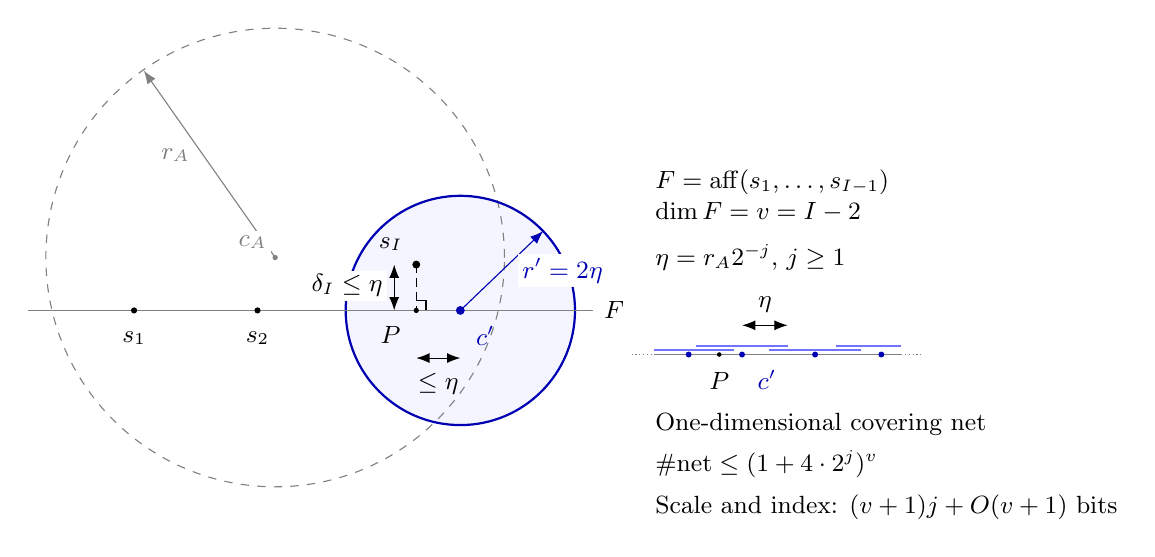
\begin{tikzpicture}[x=1.12cm,y=1.12cm,>=Latex,
  every node/.style={font=\small}]
  \fill[blue!4] (1.6,-.4) circle[radius=1.3];
  \draw[gray,dashed] (-.5,.2) circle[radius=2.6];
  \draw[blue!70!black,thick] (1.6,-.4) circle[radius=1.3];
  \draw[gray] (-3.3,-.4) -- (3.1,-.4);
  \node[anchor=west] at (3.12,-.4) {$F$};
  \node[anchor=west,align=left] at (3.7,.9)
    {$F=\operatorname{aff}(s_1,\ldots,s_{I-1})$\\
     $\dim F=v=I-2$};
  \fill (-2.1,-.4) circle[radius=.035];
  \node[below=4pt] at (-2.1,-.4) {$s_1$};
  \fill (-.7,-.4) circle[radius=.035];
  \node[below=4pt] at (-.7,-.4) {$s_2$};
  \fill (1.1,.12) circle[radius=.045];
  \node[above left=2pt] at (1.1,.12) {$s_I$};
  \draw[densely dashed] (1.1,.12) -- (1.1,-.4);
  \draw (1.1,-.29) -- (1.21,-.29) -- (1.21,-.4);
  \fill (1.1,-.4) circle[radius=.03];
  \node[below left=3pt] at (1.1,-.4) {$P$};
  \draw[<->] (.85,.12) -- (.85,-.4);
  \node[anchor=east,fill=white,inner sep=1.5pt]
    at (.77,-.12) {$\delta_I\le\eta$};
  \fill[blue!70!black] (1.6,-.4) circle[radius=.05];
  \node[below right=3pt,blue!70!black] at (1.6,-.4) {$c'$};
  \draw[<->] (1.1,-.94) -- (1.6,-.94);
  \node[below=2pt] at (1.35,-.94) {$\le\eta$};
  \draw[blue!70!black,->] (1.6,-.4) -- (2.54,.5);
  \node[anchor=west,blue!70!black,fill=white,inner sep=1.5pt]
    at (2.25,.05) {$r'=2\eta$};
  \draw[gray,->] (-.5,.2) -- (-1.99,2.32);
  \fill[gray] (-.5,.2) circle[radius=.03];
  \node[above left=2pt,gray,fill=white,inner sep=1.5pt]
    at (-.5,.2) {$c_A$};
  \node[anchor=east,gray] at (-1.36,1.36) {$r_A$};
  \node[anchor=west,align=left] at (3.7,.2)
    {$\eta=r_A2^{-j}$, $j\ge1$};
  \begin{scope}[shift={(3.8,-.9)},x=.58cm,y=.58cm]
    \draw[gray] (0,0) -- (5.4,0);
    \draw[gray,densely dotted] (-.5,0) -- (0,0);
    \draw[gray,densely dotted] (5.4,0) -- (5.9,0);
    \draw[blue!55,thick] (0,.10) -- (1.75,.10);
    \draw[blue!55,thick] (.92,.18) -- (2.92,.18);
    \draw[blue!55,thick] (2.52,.10) -- (4.52,.10);
    \draw[blue!55,thick] (3.97,.18) -- (5.4,.18);
    \foreach \x in {.75,1.92,3.52,4.97}
      \fill[blue!70!black] (\x,0) circle[radius=.065];
    \fill (1.42,0) circle[radius=.05];
    \node[below=3pt] at (1.42,0) {$P$};
    \node[below right=3pt,blue!70!black] at (1.92,0) {$c'$};
    \draw[<->] (1.92,.64) -- (2.92,.64);
    \node[above=1pt] at (2.42,.64) {$\eta$};
  \end{scope}
  \node[anchor=north west,align=left] at (3.7,-1.45)
    {One-dimensional covering net\\[4pt]
     $\#\text{net}\le(1+4\cdot2^j)^v$\\[4pt]
     Scale and index: $(v+1)j+O(v+1)$ bits};
\end{tikzpicture}
\caption{Predecessor-span localization, shown schematically in two
dimensions. Only the projection of \(s_I\) onto \(F\) is quantized:
the projected point \(P\) lies in the radius-\(2r_A\) ball about
\(s_1\) in the \(v\)-dimensional span. A fixed \(\eta\)-cover supplies
the first qualifying ordered net point \(c'\); the inset illustrates
part of such a cover in one dimension, with omitted stretches dotted.
Both errors are at most \(\eta\), so \(B(c',2\eta)\) contains \(s_I\).
The scale and net index have the displayed code-length bound, with
dimension \(v\). The new radius does not increase, but the new ball
need not lie inside the old one.}
\label{l:span:net-figure}
\end{figure}

For \(j\ge1\),
\(j\log2\le\Delta_I<(j+1)\log2\).  Thus
\[
 \log r_A-\Delta_I\le \log r'
       \le\log r_A-\Delta_I+2\log2.
\]
For \(j=0\), either \(\Delta_I=0\) or \(\Delta_I<\log2\), and the
same upper bound holds with \(r'=r_A\).  These inequalities give
\eqref{l:span:radius} and, using the finite expectations already
proved, \(\mathbb E|\log r'|<\infty\).

Encode \(j\) by the unary prefix code of length \(j+1\) bits.
For \(j\ge1\), append a fixed-length net index of
\(\lceil v\log_2(1+4\cdot2^j)\rceil\) bits.  Given \(A_*\), the
dimension \(v\) is known, so the combined code is prefix-free.
Since \(1+4\cdot2^j\le5\cdot2^j\), its length is at most
\((1+v)j+C v+2\).  Now \(1+v\le p\) and
\(j\log2\le\Delta_I\), so its expected length in nats is at most
\(p\mathbb E\Delta_I+C_1p\).  We give the countable conditional
entropy step explicitly.  For a conditioning value \(a_*\) with finite
conditional expected length, let \(\ell_{a_*}(c)\) be the bit length
and let \(p_{a_*}(c)\) be the conditional code distribution.  Kraft's
inequality \cite{Kraft1949}, in the finite or countable form stated in
\cite[Section~2.4.2, Theorem~2.4.2]{Duchi2023}, gives
\[
 0<K_{a_*}:=\sum_c2^{-\ell_{a_*}(c)}\le1.
\]
Normalize \(q_{a_*}(c)=2^{-\ell_{a_*}(c)}/K_{a_*}\).  Its cross entropy is
\[
 \sum_c p_{a_*}(c)\log\frac1{q_{a_*}(c)}
 =(\log2)\mathbb E[\ell_{a_*}(C)\mid a_*]+\log K_{a_*}
 \le(\log2)\mathbb E[\ell_{a_*}(C)\mid a_*]<\infty.
\]
For a finite partition of the code alphabet with one remaining tail
atom, nonnegative relative entropy bounds the partition entropy by
its \(q_{a_*}\) cross entropy, and that cross entropy is at most the
displayed full cross entropy.  Refining such partitions gives the
countable entropy by monotone convergence.  Hence
\(H(C\mid a_*)\le(\log2)\mathbb E[\ell_{a_*}(C)\mid a_*]\).
Finite conditional expected length holds for almost every \(a_*\)
because its average is finite.  Averaging proves the first inequality
in \eqref{l:span:code}.

Gram--Schmidt with fixed conventions supplies measurable
orthonormal coordinates from the predecessor differences, and the
fixed ordering resolves net ties.  Define the code arbitrarily on
the null degeneracy set.  The decoded ball is therefore measurable.
The pointwise construction puts \(s_I\) in that decoded ball outside
the null degeneracy set.  The event
\(\{\|s_I-c'(A')\|\le r'(A')\}\) is Borel and has probability one.
Disintegrating it over \(A'\) shows that its conditional probability
is one for almost every \(A'\).  Thus the decoded ball supports the
conditional signal law.
Conditioning an absolutely continuous law on a discrete code keeps
absolute continuity almost surely.  The conditional entropy chain
rule gives the second inequality in \eqref{l:span:code}, and its
finite right side proves the remaining finiteness claim.
\end{proof}

\subsection{The sample bound}

The preceding two lemmas now give a complete potential argument.
The result uses the local model and the local cap and full-data
calculation of Section~\ref{l:model}; the only companion input remains
\eqref{l:span:equal-label-input}.

\begin{proposition}[A predecessor-span block bound]
\label{l:span:block-bound}
For sufficiently large \(d\), put \(K=p=\lfloor d/8\rfloor\).
Consider a learner of Section~\ref{l:model} with horizon \(T\) and
\(M\) persistent bits, and set \(W=(T+2)2^M\).  If
\(\log W\le2d^2\), then its uniform-sphere angular success
probability \(\pi\) at \(0<\epsilon\le1/10\) satisfies
\begin{equation}
 \pi(d-1)\log(1/\epsilon)
 \le C d\left(\left\lceil T/K\right\rceil+1\right)
 \label{l:span:success-bound}
\end{equation}
for an absolute \(C\).  In particular, success at least \(2/3\)
implies
\[
 \left\lceil T/K\right\rceil
       \ge c\log(1/\epsilon)-C'
\]
with absolute \(c>0,C'>0\).
\end{proposition}
\begin{proof}
Condition on the shared rule randomness.  For almost every value, the
joint initialization independence in Section~\ref{l:model} leaves
the initial state independent of the signal and all sample rows.
By Lemmas~\ref{l:borel} and \ref{l:prior-ac}, the conditional
uniform-prior experiment has Borel rule versions.  We prove the
displayed numerical bound for each such value, with its conditional
success probability.  Averaging that bound at the end handles shared
randomness without requiring jointly selected Borel versions.

Pad an early-stopping program to \(T\) observations by retaining its
terminal state and stopping index, and then ignoring the remaining
pairs.  At each index the padded state has at most \(W\) values, and
the final output law uses only that state.  Divide the observations
into blocks of length \(K\), allowing a shorter final block.  Set
\[
 a=K+p,\qquad
 \Phi(A,r_A)=\mathcal D(A)+a\mathbb E\log r_A.
\]
For every nonempty block length \(1\le k\le K\), the inequalities
\(k+p+1<d\) and \(a\le(d-1)/2\) hold once \(d\) is sufficiently
large.  Initially \(A\) is the signal-independent initial state and
the containing ball is \(B(0,1)\), so \(\Phi=0\).

At a block, select a replica and encode its new ball as above.
Combining \eqref{l:span:selected-bound}--\eqref{l:span:code} gives
\begin{align}
 \Phi(A',r')
 &\le\Phi(A,r_A)+\frac{\log W}{p}+\frac{k}{2}+C_1p+2a\log2
           +(k+p-a)\mathbb E\Delta_I \notag\\
 &\le\Phi(A,r_A)+C_2d.
 \label{l:span:drift}
\end{align}
Indeed \(k+p-a\le0\), while \(p\ge d/16\) and
\(\log W\le2d^2\) make the width charge \(O(d)\).
The cancellation has a direct explanation: the likelihood
charges \(k\Delta_I\), the code charges at most \(p\Delta_I\), and
the radius credit is \(a\Delta_I=(K+p)\Delta_I\).

Every posterior draw has the correct joint marginal with the block
destination.  Uniformly selecting one draw therefore preserves the
learner's state--signal marginal, and recording its code changes no
marginal law.  Generate the next Gaussian block independently of the
pair consisting of the current signal and augmented analysis
variables.  Since the learner's transition uses
the past only through its state, induction preserves the actual
state--signal marginal at every boundary.  The predecessor points
and codes are never given to the learner.  All required finiteness
properties propagate by Lemma~\ref{l:span:localization}.  Thus after
\(b=\lceil T/K\rceil\) blocks,
\[
 \Phi\le C_2db.
\]
For \(T=0\) this holds directly with \(b=0\).

Write \(n=d-1\).  Lemma~\ref{l:caps-endpoint} gives
\(\mu(B(c_A,r_A))\le(2r_A)^n\).  A density supported in a set \(E\)
has relative entropy at least \(-\log\mu(E)\), by comparison with
\(\mu(\,\cdot\mid E)\).  Therefore
\[
 D(f_A\mu\|\mu)\ge-n\log(2r_A)
\]
almost surely, and
\begin{equation}
 \Phi\ge\left(1-\frac an\right)\mathcal D(A)-a\log2
       \ge\frac12\mathcal D(A)-a\log2.
 \label{l:span:coercivity}
\end{equation}
The unconditional signal law remains \(\mu\), so
\(\mathcal D(A)=I(S;A)\).  The final \(A\) includes the padded state
\(w\), and hence \(\mathcal D(A)\ge I(S;w)\).

Under the product of \(\mu\) and the output marginal, angular
success has probability at most \(\epsilon^n\), by
Lemma~\ref{l:caps-endpoint}.  Data processing through the terminal
output and then through the success event gives
\[
 I(S;w)\ge I(S;\widehat S)
       \ge \pi n\log(1/\epsilon)-\log2
\]
by \eqref{l:binary}.  This holds with the success probability for
the fixed shared seed.  Combining it with the potential upper bound
and \eqref{l:span:coercivity} proves
\eqref{l:span:success-bound} with constants independent of that
seed.  Averaging proves the asserted bound for the original shared
randomness as well.
\end{proof}

\begin{theorem}[The full accuracy range by predecessor-span localization]
\label{l:span:theorem}
Let \(M(d)=o(d^2)\) be integer-valued and let
\(0<\epsilon(d)\le1/10\).  A family of learners in
Section~\ref{l:model} whose angular success probability is at least
\(2/3\) for a uniform spherical signal must use
\[
 T(d)\ge c\,d\log(1/\epsilon(d))
\]
for all sufficiently large \(d\), where \(c>0\) is absolute.
The eventual threshold may depend on the memory sequence.  The
same conclusion follows from success at least \(2/3\) for every
fixed signal.
\end{theorem}
\begin{proof}
Put \(L=\log(1/\epsilon)\ge\log10\).  The last statement follows by
averaging over the uniform signal, so it suffices to prove the average
statement.  There are at most \((T+1)2^M\) terminal time--state
pairs.  For each fixed pair its fresh output law succeeds on uniform
mass at most \(\epsilon^{d-1}\), by the cap bound and integration
over that output law.  More explicitly, for a terminal pair \(h\)
let \(a_h(s)\) be that fixed output law's success probability at
signal \(s\), and let \(t_h(s)=\Pr(h\text{ is reached}\mid S=s)\).
The pair's contribution is
\[
 \int t_h(s)a_h(s)\,\mu(ds)
 \le\int a_h(s)\,\mu(ds)\le\epsilon^{d-1},
\]
because \(0\le t_h(s)\le1\).  Summing over all pairs, for almost
every shared seed and hence after averaging, yields
\[
 \frac23\le (T+1)2^M\epsilon^{d-1}.
\]
Equivalently,
\begin{equation}
 (d-1)L\le M\log2+\log(T+1)+\log(3/2).
 \label{l:span:output-count}
\end{equation}

At indices where \(T\ge dL\) the conclusion is immediate.  At the
other indices, \eqref{l:span:output-count} gives
\[
 (d-1)L\le M\log2+\log(dL+1)+\log(3/2).
\]
For all sufficiently large \(d\), uniformly for \(L\ge\log10\),
\(\log(dL+1)\le dL/6\), while \((d-1)L\ge dL/2\).
Consequently \(dL\le3M\log2+3\log(3/2)=o(d^2)\) along such
short indices.  In particular \(\log((T+2)2^M)\le2d^2\) eventually,
so Proposition~\ref{l:span:block-bound} applies.  It gives
\[
 T\ge K\{c_0L-C_0-1\}
\]
with absolute \(c_0>0,C_0\).  Above a sufficiently large absolute
threshold for \(L\), use \(K\ge d/16\) and absorb the constants to
obtain \(T\ge c_1dL\).

For completeness, the local full-data argument supplies the remaining
constant-accuracy range with explicit constants.  If \(T\le d/8\),
reveal every row and label.  The conditional unknown component is
uniform on a residual sphere of radius \(R\).  By isotropy and
Markov's inequality,
\[
 \Pr\{R<1/2\}\le \frac{4T}{3d}\le\frac16.
\]
On \(R\ge1/2\), antipodal residual points correspond to signals
separated by at least one, so a radius-\(\epsilon\) error ball with
\(\epsilon\le1/10\) contains at most one point of each pair.
Conditional success is at most \(1/2\), also for a randomized
estimate.  Total success is at most
\[
 \frac16+\frac56\cdot\frac12=\frac7{12}<\frac23.
\]
Thus \(T>d/8\).  This proves \(T\ge c_2dL\) throughout the bounded
range of \(L\) left above.  Taking the minimum of the absolute
constants completes the proof, including nonmonotone accuracy
sequences and early stopping.
\end{proof}

\section{A convex potential from inverse-distance kernels}\label{lk:section}

Explicit revelations are one way to pay for a concentrated posterior.
This section uses a different accounting method. From the relative
entropy of a posterior we subtract the logarithm of an inverse-distance
average. The resulting functional is convex, so after a block we may
forget the entering state without increasing it. A mixed projection
estimate then charges only the rows that the learner actually saw.

Throughout this section, \(\sigma\) is uniform probability on
\(S^{d-1}\), \(n=d-1\), \(k=\lfloor d/16\rfloor\), and \(p=2k\).
We work in sufficiently large dimension that \(k\ge1\) and \(2p<n\).
For a probability measure \(\nu\le H\sigma\), \(H<\infty\), put
\begin{equation}\label{lk:definition}
 J_\nu(s)=\int\|u-s\|^{-p}\,d\nu(u),\qquad
 B(\nu)=\int\log J_\nu(s)\,d\nu(s),\qquad
 \Phi(\nu)=D(\nu\|\sigma)-B(\nu).
\end{equation}
The sphere has diameter two, so \(J_\nu\ge2^{-p}\). The centered
ball bound of Lemma~\ref{l:caps-endpoint}, summed on dyadic annuli,
bounds \(J_\nu\) above uniformly in \(s\) because \(p<n\).
Thus every term in \eqref{lk:definition} is finite.

\Needspace{6\baselineskip}
\begin{lemma}[Convexity and coercivity]\label{lk:coercive}
The functional \(\Phi\) is convex under finite mixtures of
bounded-density probability measures and
\[
 \Phi(\nu)\ge\tfrac12D(\nu\|\sigma)-Cd,\qquad
 \Phi(\sigma)\le p\log2
\]
for an absolute \(C\).
\end{lemma}
\begin{proof}
Writing \(f=d\nu/d\sigma\), we have
\(\Phi(\nu)=\int f\log(f/J_\nu)\,d\sigma\), with value zero where
\(f=0\). Both \(f\) and \(J_\nu\) are linear in \(\nu\).
For \(x>0,y>0\), the Hessian of \(x\log(x/y)\) has quadratic form
\((a-bx/y)^2/x\); continuity at \(x=0\) gives joint convexity on
\(x\ge0,y>0\). Integration proves the mixture assertion.

By Jensen and rotational invariance,
\[
 \int J_\nu(s)^2\,d\sigma(s)
 \le\int\!\int\|u-s\|^{-2p}\,d\sigma(s)d\nu(u)
 \le e^{Cd}.
\]
For the last bound, distances greater than one contribute at most
one. On \(2^{-i-1}<\|u-s\|\le2^{-i}\), the contribution is at most
\(2^{2p}2^{-i(n-2p)}\); its sum converges since \(n-2p>0\).
Apply the entropy inequality \eqref{l:tilt}, equivalently
\(\E_\nu F\le D(\nu\|\sigma)+\log\E_\sigma e^F\), to
\(F=2\log J_\nu\). This logarithm is bounded for fixed \(\nu\).
It gives \(2B(\nu)\le D(\nu\|\sigma)+Cd\). Finally,
\(D(\sigma\|\sigma)=0\) and \(J_\sigma\ge2^{-p}\).
\end{proof}

\subsection{Exact projection densities and the kernel entropy}

We will use differential entropy of exact labels. The following
elementary density statement fixes both its version and its
integrability before the information identity is used.

\begin{lemma}[Projection versions and logarithms]\label{lk:density}
Let \(1\le\ell<d-1\), let \(G\) have \(\ell\) independent standard
Gaussian rows, and let \(\nu\le H\sigma\) be a probability measure.
For each full-row-rank \(g\), the image \(g_\#\nu\) has a Lebesgue
density. The limit, where finite and existent, of
\[
 p_{\nu,a}(g,y)=(2a)^{-\ell}
     \nu\{u:\|gu-y\|_\infty\le a\},
 \qquad a=1,1/2,1/3,\ldots,
\]
and zero elsewhere is a jointly Borel density version \(p_\nu(g,y)\).
Under the independent law of \(G\) and \(S\sim\nu\),
\(\log p_\nu(G,GS)\) is integrable.

If instead \(G\) and \(S\sim\sigma\) are marginally independent and
\(W\) is finite with any joint law with them, the actual conditional
law of \(GS\) given \((G,W)\) has a Lebesgue density. Its logarithm
and \(\log p_{\nu_W}(G,GS)\), where
\(\nu_w=P_{S\mid W=w}\), are integrable under the actual law.
The same assertion holds after first conditioning on a finite entering
variable \(V\), provided the fresh \(G\) is jointly independent of
\((S,V)\). Equivalently, conditional on each positive-probability value
of \(V\), the joint law of \((G,S)\) must be the product of the original
Gaussian row law and the conditional law of \(S\).
\end{lemma}
\begin{proof}
Writing \(H_g=(gg^{\mathsf T})^{1/2}\), an orthogonal change of
coordinates and a nonsingular change of label coordinates give
\[
 p_\sigma(g,y)=
 \frac{c_{d,\ell}}{\det(gg^{\mathsf T})^{1/2}}
 \left(1-\|H_g^{-1}y\|^2\right)^{(d-\ell-2)/2}
 \ind_{\{\|H_g^{-1}y\|<1\}}.
\]
The spherical coordinate formula follows by splitting a normalized
standard Gaussian into its \(\ell\) row-space coordinates and the
remaining coordinates: the squared projected length is
\(\operatorname{Beta}(\ell/2,(d-\ell)/2)\). Domination proves absolute
continuity for \(\nu\). Lebesgue differentiation proves the claim
about cube limits, and their defining integrals are jointly Borel.

Under \(G\otimes\sigma\), the logarithm in the displayed formula is
integrable. The beta density has integrable logarithms at its two
endpoints. Gram--Schmidt expresses \(\det(GG^{\mathsf T})\) as a
product of chi-square variables of positive degrees, each with
integrable logarithm. Domination by \(H\) preserves this baseline
integrability for \(S\sim\nu\). The projected likelihood ratio
\(p_\nu/p_\sigma\) has relative entropy at most
\(D(\nu\|\sigma)\le\log H\) by data processing. Its negative
logarithmic part has expectation at most \(1/e\), since
\(t\log^-(t)\le1/e\) under the probability reference. Its positive
part is then finite as well. This proves the first integrability
assertion.

For a positive-probability \(w\), the actual law of \((G,S)\) given
\(w\) is dominated by \(P(W=w)^{-1}\) times \(G\otimes\sigma\).
Its image therefore has a density, and the baseline logarithm is
integrable; averaging over \(w\) restores its original finite
expectation. The log ratio of the actual image density to
\(p_\sigma\) has relative entropy \(I(W;GS\mid G)\le H(W)\) and
negative part at most \(1/e\). Thus the actual log density is
integrable. Moreover,
\[
 \E D(P_{S\mid G,W}\|\nu_W)=I(S;G\mid W)\le H(W),
\]
where the last inequality uses \(I(S;G)=0\) and the chain rule.
Data processing under \(s\mapsto Gs\) gives integrability of the
log ratio between the actual image density and \(p_{\nu_W}\);
subtracting it proves the remaining claim. If a finite entering
variable is first fixed, its signal law is bounded relative to
\(\sigma\), and the same argument applies to each positive-probability
case and then to their finite average.
\end{proof}

\begin{lemma}[The kernel controls projection entropy]\label{lk:entropy}
Let \(X\) have \(p\) independent standard Gaussian rows and be
independent of \(S\sim\nu\le H\sigma\), \(H\ge1\). For a sufficiently
large absolute \(C_0\), put
\(b_H=\lceil C_0(d+\log(2H))\rceil\). Then
\[
 h(XS\mid X)\le -B(\nu)+Cd+2\log(b_H+2).
\]
\end{lemma}
\begin{proof}
For \(r_i=2^{1-i}\), let \(m_i(s)=\nu(B(s,r_i))\).
Dyadic shells give
\[
 J_\nu(s)\le 2^p\sum_{i\ge0}r_i^{-p}m_i(s).
\]
Since \(m_i(s)\le H(2r_i)^n\) and \(n-p\ge1\), choosing \(C_0\)
large makes the sum over \(i>b_H\) at most \(2^{-p}\).
The term \(i=0\) is itself \(2^{-p}\). Choose the first maximizer
\(j=j(s)\le b_H\). This is measurable and satisfies
\[
 \log(r_j^{-p}m_j(s))
 \ge\log J_\nu(s)-Cd-\log(b_H+2).
\]

For fixed \(X\), compare the actual projected density to
\[
 Q_X(y)=\frac1{b_H+1}\sum_{i=0}^{b_H}
       \int \gamma_{r_i}(y-Xu)\,d\nu(u),
\]
where \(\gamma_r\) is the \(N(0,r^2I_p)\) density. At \(y=Xs\),
retain the \(j\)-summand and restrict it to \(B(s,r_j)\).
Jensen's inequality for the logarithm on that normalized restriction
and \(\E_X\|X(s-u)\|^2=p\|s-u\|^2\le pr_j^2\) give
\[
 \E_X\log Q_X(Xs)
 \ge\log(r_j^{-p}m_j(s))-\log(b_H+1)
     -\tfrac p2\log(2\pi)-\tfrac p2.
\]
Integrate over \(s\). The comparison density has finite cross
entropy by this bound and its finite Gaussian-mixture upper bound.
The actual differential entropy is finite by Lemma~\ref{lk:density}.
Nonnegativity of relative entropy to \(Q_X(y)\,dy\) proves the result.
\end{proof}

\subsection{The mixed estimate and the actual-row charge}

The following is the positive-scale assertion of
\cite[Theorem~3.1]{OpenAIRow2026}. We state its parameters explicitly
because its application has only one unit of angular slack. Its proof
is in that companion; the reweighting and change of row law below are
proved here.

\begin{theorem}[Mixed projection estimate]\label{lk:mixed-input}
Let \(m,r,q\ge1\) be integers, \(\ell=m+r<n=d-1\), and
\(\ell-m-(q-1)\ge1\). Let \(\rho\) be a finite measure on the sphere
such that, for every ambient \(z\) and \(t>0\),
\(\rho(B(z,t))\le Bt^\ell\) and
\(\rho(B(z,t))\le Dt^n\), with \(B,D>0\). For independent Gaussian
matrices \(X,Z\) with \(m,r\) rows, put \(G=(X;Z)\) and
\[
 p_{\rho,\delta}(G,y)=(2\delta)^{-\ell}
      \int\ind_{\{\|Gu-y\|_\infty\le\delta\}}\,d\rho(u).
\]
For every fixed \(s\in S^{d-1}\) and every \(\delta>0\),
\[
 \left[\E_X\left(\E_Zp_{\rho,\delta}(G,Gs)\right)^q\right]^{1/q}
 \le e^{Cd}B\bigl(1+\log^+(D/B)\bigr).
\]
\end{theorem}

The estimate is for positive cube averages and every fixed signal.
In its use below, we first change the law of the actual rows while
\(\delta>0\), and only then pass to exact labels under their actual
law. No assertion about a fixed-signal value of an arbitrary density
version is used.

\begin{lemma}[Reweighting by the potential]\label{lk:reweight}
For \(\nu\le H\sigma\), define \(d\rho=d\nu/J_\nu\). Then
\[
 \rho(B(z,r))\le(2r)^p,\qquad \rho\le2^pH\sigma.
\]
By Theorem~\ref{lk:mixed-input}, for independent \(k\)-row
Gaussian matrices \(A,A'\), \(X=(A;A')\), every \(s\in\sphere\), and
every \(\delta>0\),
\begin{equation}\label{lk:moment}
 \left[\E_A\left(\E_{A'}p_{\rho,\delta}(X,Xs)\right)^k\right]^{1/k}
 \le e^{Cd}(b_H+2).
\end{equation}
\end{lemma}
\begin{proof}
For \(s\in B(z,r)\), \(J_\nu(s)\ge(2r)^{-p}\nu(B(z,r))\).
Integrating its reciprocal over the ball proves the first inequality;
if the ball has zero \(\nu\)-mass there is nothing to prove. The second
uses \(J_\nu\ge2^{-p}\).

Apply Theorem~\ref{lk:mixed-input} with
\(m=r=q=k\), \(\ell=p=2k\), \(B=2^p\), and
\(D=2^{p+n}H\), using the ambient-center cap bound of
Lemma~\ref{l:caps-endpoint}. The angular margin is exactly
\(p-k-(k-1)=1\), and the radial margin is \(n-p>0\).
Moreover \(1+\log^+(D/B)\le C(d+1+\log H)\le C(b_H+2)\);
the factor \(2^p\) is absorbed in \(e^{Cd}\). This proves
\eqref{lk:moment}. The local inverse factor behind this substitution
is \(\|u-s\|^{-k}\dist(u-s,E)^{-k}\), where \(E\) is a linear
subspace with \(\dim E\le k-1\).
\end{proof}

\begin{proposition}[Drift of the kernel functional]\label{lk:drift}
Let \(S\sim\sigma\), let
\(V\) have at most \(N\) values, and let a \(k\)-row Gaussian
matrix \(A\) be independent of \((S,V)\). Suppose \(W\) has at most
\(N\) values and is generated by a Borel probability kernel of
\((V,A,AS)\) and independent randomness. If \(\log N\le d^2\),
then, for sufficiently large \(d\),
\[
 \E\Phi(P_{S\mid W})\le \E\Phi(P_{S\mid V})+Cd.
\]
\end{proposition}
\begin{proof}
Condition first on \(V=v\) with positive probability. Put
\(\nu=P_{S\mid v}\) and \(H_v=P(V=v)^{-1}\). In this conditional
experiment \(w\) always ranges over values with \(P(V=v,W=w)>0\);
for these values put
\(\nu_w=P_{S\mid v,w}\) and \(H_{vw}=P(V=v,W=w)^{-1}\).
The two posteriors are bounded by \(H_v\sigma\) and
\(H_{vw}\sigma\). Introduce a \(k\)-row Gaussian matrix \(A'\)
independent of \((S,V,A,W)\), and put \(X=(A;A')\), \(Y=XS\).
Within the conditional experiment \(X\) is independent of \(S\),
and \(W\) depends on \(S\) only through \((X,Y)\). The chain rule gives
\begin{equation}\label{lk:identity}
 I(S;W)=h(Y\mid X)-h(Y\mid X,W)-I(X;S\mid W).
\end{equation}
For example,
\(I(S;W)=I(X,Y;W)-I(X;W\mid S)\), and \(I(X;S)=0\)
converts the difference of the two row-information terms into
\(-I(X;S\mid W)\). All displayed differential entropies are finite
by Lemma~\ref{lk:density}, and \(I(X;S\mid W)\le H(W)\).

For fixed \(w\), use the finite nonzero measure
\(\rho_w=\nu_w/J_{\nu_w}\) as a reference, and write
\(a_w=\rho_w(\sphere)\). First normalize this reference.
The relative entropy of the actual conditional law of \((X,S)\)
with respect to \(P_{X\mid w}\otimes(\rho_w/a_w)\) is
\[
 I(X;S\mid w)+B(\nu_w)+\log a_w<\infty.
\]
Indeed, \(\log J_{\nu_w}\) is bounded for this \(v,w\), and
\(I(X;S\mid w)<\infty\). Probability data processing under
\((X,s)\mapsto(X,Xs)\) makes the corresponding post-map relative
entropy finite. For probability laws \(P\ll Q\), the elementary bound
\[
 \int_{\{dP/dQ<1\}}-\log(dP/dQ)\,dP\le 1/e
\]
shows that a finite relative entropy has an integrable log density
ratio. The post-map ratio is the actual conditional label density
divided by \(p_{\rho_w}(X,Y)/a_w\). Its logarithm is therefore
integrable. Lemma~\ref{lk:density} makes the logarithm of the actual
conditional label density integrable as well, so
\(\log p_{\rho_w}(X,Y)\) is integrable under the actual conditional
law. Here \(p_{\rho_w}\) is the cube-limit density version; the same
construction applies to a finite measure.

We may now expand both finite-reference divergences and subtract
\(\log a_w\) from probability data processing. Before the map the
divergence is \(I(X;S\mid w)+B(\nu_w)\), while after the map it is
\(-h(Y\mid X,w)-\E[\log p_{\rho_w}(X,Y)\mid w]\). Consequently,
\begin{equation}\label{lk:finite-reference}
 -h(Y\mid X,w)-I(X;S\mid w)
 \le B(\nu_w)+\E[\log p_{\rho_w}(X,Y)\mid w].
\end{equation}
This is precisely the finite-reference data-processing statement
proved in Section~\ref{l:model}, including when \(\rho_w\) has mass
greater than one.

We now bound the last logarithm under the selected actual rows. Let
\(Q\) be the original Gaussian law of \(A\), still conditional on
\(v\), and write \(\kappa_w(a,as)\) for the Borel block probability
of message \(w\). For \(r_w(s)=\int\kappa_w(a,as)\,Q(da)>0\), choose
the conditional row law
\[
 Q_{s,w}(da)=\frac{\kappa_w(a,as)}{r_w(s)}\,Q(da);
\]
when \(r_w(s)=0\), assign \(Q_{s,w}=Q\). The normalizer is positive
for almost every \((s,w)\) under the actual law, and this is a
conditional version of the row law there. In particular
\(Q_{s,w}\ll Q\). Also
\[
 \E_{s,w}D(Q_{s,w}\|Q)=I(A;W\mid S)\le H(W)\le\log N,
\]
so the divergence is finite for almost every \((s,w)\) under that law.
The fresh \(A'\) retains its independent Gaussian law after
conditioning on \((A,s,w)\). For almost every such pair and for
\(\delta>0\), Jensen in \(A'\), followed by \eqref{l:tilt}
with exponent \(k\), gives
\begin{align}
 &\E[\log(1+p_{\rho_w,\delta}(X,Xs))\mid s,w]\notag\\
 &\quad\le\frac{D(Q_{s,w}\|Q)}k+
 \frac1k\log\E_{A\sim Q}
       \left(1+\E_{A'}p_{\rho_w,\delta}(X,Xs)\right)^k\notag\\
 &\quad\le\frac{D(Q_{s,w}\|Q)}k+Cd+\log(b_{H_{vw}}+2).
 \label{lk:row-charge}
\end{align}
The last step uses the \(L^k\) triangle inequality and
\eqref{lk:moment}, whose fresh moment holds for every fixed
\(s\in\sphere\). The displayed row-charge inequality is used only
for almost every \((s,w)\) under the actual law, while \(\delta\)
is positive.

Here is the exact null-set transfer in that passage. For each
full-rank \(X\), Lebesgue differentiation makes
\(p_{\rho_w,1/a}(X,y)\) converge to \(p_{\rho_w}(X,y)\)
for Lebesgue-almost every \(y\). The failure set is jointly Borel
by the cube definitions. Under the actual conditional law given
\((v,w)\), \((X,S)\) is dominated by a finite multiple of
\(\gamma_p\otimes\sigma\); pushing forward shows that \((X,Y)\)
is absolutely continuous with respect to \(\gamma_p(dX)\,dy\).
Consequently it avoids this failure set, including after the actual
rows have been tilted by \(w\). Fatou applied to the nonnegative
\(\log(1+p_{\rho_w,1/a}(X,Y))\), after integrating \eqref{lk:row-charge}
over \(s,w\), proves the same integrated upper bound for
\(\log(1+p_{\rho_w}(X,Y))\), and hence for \(\log p_{\rho_w}\).
This argument does not invoke an unsmoothed moment at
\(\rho_w\)-almost every fixed signal.

The preceding estimate supplies the quantitative positive-log bound;
integrability of both signs was established before
\eqref{lk:finite-reference}. Substituting
Lemma~\ref{lk:entropy} and
\eqref{lk:finite-reference}--\eqref{lk:row-charge} into
\eqref{lk:identity}, and using
\(I(S;W)=\E_wD(\nu_w\|\sigma)-D(\nu\|\sigma)\), yields
\[
 \E_w\Phi(\nu_w)\le\Phi(\nu)+Cd+2\log(b_{H_v}+2)
       +\E_w\log(b_{H_{vw}}+2)+\frac{\log N}{k}.
\]
Restore the average over \(v\).
\(\E\log H_V=H(V)\le\log N\) and
\(\E\log H_{VW}=H(V,W)\le2\log N\). Jensen bounds the averaged
cutoff terms by \(C\log(d+1+2\log N)\), while
\(\log N/k\le Cd\). For fixed \(w\), \(P_{S\mid W=w}\) is the
finite mixture of \(\nu_w=P_{S\mid v,w}\) over \(v\).
Lemma~\ref{lk:coercive} permits forgetting \(v\), proving the drift.
\end{proof}

\subsection{Precision and the global stopping index}

\begin{corollary}\label{lk:regression}
Let \(M(d)=o(d^2)\) and
\(0<\epsilon(d)\le1/10\). A learner in the model of
Section~\ref{l:model} with uniform-sphere average angular success at
least \(2/3\) requires
\(T(d)\ge c d\log(1/\epsilon(d))\) for an absolute \(c>0\)
in sufficiently large dimension. The threshold may depend on the
memory sequence.
\end{corollary}
\begin{proof}
Fix the shared rule randomness with uniform-prior success at least
\(2/3\), and apply Lemmas~\ref{l:prior-ac} and~\ref{l:borel}.
Keep the internal transition and output randomness. Put
\(L=\log(1/\epsilon)\). Under the product of the marginal laws of
\((S,\widehat S)\), angular success has probability at most
\(\epsilon^{d-1}\), by Lemma~\ref{l:caps-endpoint}.
Equation~\eqref{l:binary} therefore gives
\begin{equation}\label{lk:output}
 I(S;\widehat S)\ge\tfrac23(d-1)L-\log2.
\end{equation}

Assume \(T<dL\). The other case is already sufficient. The terminal
state and stopping index have at most \((T+1)2^M\) values, so the
left side of \eqref{lk:output} is at most
\(M\log2+\log(T+1)\). Since
\(\log(T+2)\le C+\log d+\log(L+1)\le C+\log d+L\),
absorption gives
\[
 L\le C\frac{M+1+\log d}{d},\qquad T=O(d+M).
\]
For \(M=o(d^2)\), pad stopped states with their original terminal
labels and indices and add unused rows to complete the last block.
Every padded layer has at most \(N=(T+2)2^M\) states and
\(\log N=o(d^2)\).

The initial conditional signal law is \(\sigma\), because the model
makes initialization independent of the signal conditional on the
fixed shared rule randomness. Iterate
Proposition~\ref{lk:drift} for \(\lceil T/k\rceil\) blocks and apply
Lemma~\ref{lk:coercive}. For the final padded state \(F\),
\[
 I(S;F)=\E D(P_{S\mid F}\|\sigma)
 \le Cd\bigl(1+\lceil T/k\rceil\bigr).
\]
The output is generated from \(F\) and fresh randomness. Data
processing with \eqref{lk:output} gives
\(L\le C(1+T/d)\). The \(2/3\) instance of
Lemma~\ref{l:caps-endpoint} gives \(T>d/4\) for this same prior
and exact observation model. Thus \(1+T/d\le5T/d\), proving the
claimed sample bound. The global-clock calculation controls only
the padded width; the precision-dependent conclusion comes from
the block drift.
\end{proof}

\section{Maximum cell mass and inverse volumes at all scales}\label{lc:cell}

This section gives an independent proof of the uniform-sphere sample
lower bound in Corollary~\ref{lk:regression}. We track what the complete
boundary-state history reveals about the signal, subtracting a
correction built from local cell masses. The correction accounts for
concentration already present in the conditional signal law. Its
geometric input controls inverse simplex volumes without any
bounded-support assumption.

After the model and stopping reductions below,
Section~\ref{lc:cell-selection} establishes coercivity of the correction,
Section~\ref{lc:cell-inverse-section} proves the inverse-volume bound
without a support restriction, Section~\ref{lc:cell-fibers} compares
incoming and outgoing exact-observation fibers, and
Section~\ref{lc:cell-endgame} completes the information-growth and
decoding estimates.

The information identities below are the conditional relative-entropy chain rule; see \cite[Section~3.3]{Austin2020} for its standard Borel formulation. All fiber comparisons needed here are proved explicitly.

We use uniform probability \(\sigma\) on \(S^{d-1}\) for the signal,
written \(U\) when random. All logarithms are natural except in dyadic
scale definitions. Set \(L=\log(1/\epsilon)\), and suppose
\(M=M(d)=o(d^2)\) and \(0<\epsilon\le1/10\). Work in sufficiently
large dimension that \(M\le d^2\).

Assume uniform-prior angular success at least \(2/3\) in the model of
Section~\ref{l:model}. Fix the shared rule randomness with success
strictly greater than \(3/5\). Lemmas~\ref{l:prior-ac} and~\ref{l:borel}
replace those fixed rules by everywhere Borel rules for this prior.
Then fix the initial state and the independent transition and output
seeds with success at least \(3/5\). The resulting deterministic
program has the same state bound. Its output is determined by its
terminal state and index.

We may assume \(T<dL\). Otherwise the desired lower bound is immediate.
There are at most \((T+1)2^M\) possible output labels. By the cap bound
of Lemma~\ref{l:caps-endpoint}, the union of their successful signals
has mass at most \((T+1)2^M\epsilon^{d-1}\). Hence
\[
 \frac35\le (T+1)2^M\epsilon^{d-1}.
\]
Since \(L\ge\log10\) and \(T<dL\),
\(\log(T+1)\le\log(2d)+L\). Taking logarithms gives
\((d-2)L\le M\log2+\log(2d)+\log(5/3)\). Thus \(L=O(d)\) and
\(T=O(d^2)\) in the case under consideration. The \(3/5\) endpoint
in Lemma~\ref{l:caps-endpoint} also gives \(T>d/20\). These reductions
will bound the entropy of the complete boundary history; they do not
supply the precision-dependent block estimate.

\subsection{Selected cells and their entropy cost}\label{lc:cell-selection}

Use the parameters
\[
 n=k=\lfloor d/100\rfloor,\qquad \alpha=(d-1)/2.
\]
Group sample layers into blocks of size \(n\), completing the last
block with independent unused samples. In each block denote by \(A\)
the \(n\)-by-\(d\) matrix of sample rows and by \(b=AU\) the responses.
We keep, for the analysis, a history consisting of the messages at all
the block boundaries so far, starting with an empty history. Write
\(V\) for the incoming history and \(W=(V,Z)\) for the history after
the next message.

The message records the ending program state or, if the program halted
within the block, the layer of that block and final state; it can be a
dummy message in subsequent blocks. An initial state is fixed. This
scheme also permits recording if halted at the start. Thus conditional
on \(V\) there are at most \((n+2)2^M+1\) messages. Given \(V,A,b\)
the next message can be formed, and \(A\) is fresh and independent of
\(V,U\). The final history determines the output.

There are \(O(d)\) blocks by the preceding reduction. The message
alphabet therefore bounds the entropy of every history by \(O(d^3)\).
This bound will control the scale selectors below. The complete history
need not be available in program memory.

For a history \(V\), let \(p_v=\Pr(V=v)\), and write \(\mu_v\) for the conditional law of \(U\) given \(v\), with density \(f_v\) with respect to \(\sigma\). Throughout we ignore conditioning states of probability zero. These densities exist and can be taken bounded by \(1/p_v\), since the marginal law is \(\sigma\). Write \(I_V=I(U;V)=\mathbb E\log f_V(U)\); use the analogous notations for \(W\). We will track information with a correction for local concentration: a log cell-mass quantity \(J_V\) below will be subtracted from \(I_V\) in bounding its growth per block.

Define levels \(j\ge 0\) of cells of scale \(r_j=2^{1-j}\). Level 0 consists of the whole sphere. For \(j\ge 1\) use the sphere intersected with a partition into half-open grid cubes of side \(r_j/\sqrt d\). Denote the cell containing \(u\) by \(C_j(u)\); each cell has diameter at most \(r_j\) and \(\sigma\)-measure at most \((2r_j)^{d-1}\). For any of our probability laws \(\mu=\mu_v\) define
\[
 m_\mu(u)=\max_{j\ge 0} \frac{\mu(C_j(u))}{r_j^\alpha}.
\]
In fact \(m_\mu\ge 2^{-\alpha}\) and the terms for large \(j\) are bounded by \(2^{d-1} r_j^{d-1-\alpha}/p_v\). Let \(j_v(u)\) choose the first level giving the maximum. It is bounded for each \(v\) by
\[
 1+\frac{\log_2(1/p_v)+d-1+\alpha}{d-1-\alpha}.
\]
Together the selector and the selected cell define a partition for each \(v\), with parts \(D\) consisting of points having the same selector and selected cell. When speaking of the random part \(D\) we include its identification by this choice (given \(v\)). Denote by \(p_D=\mu_v(D)\) its probability, by \(j=j_v(U)\) the chosen level, and by \(p_C=\mu_v(C_j(U))\) the original cell probability. Then
\begin{equation}\label{lc:cell-eq1}
\mathbb E\log(p_C/p_D)\le H(j\mid V).
\end{equation}
Indeed conditional on \(v,j\), \(p_D\) is the selector probability given \(v\) times the probability of the cell given \(v,j\). The expected log of its ratio with \(p_C\), in the order in \eqref{lc:cell-eq1}, equals the surprisal of the selector given \(v\) minus a nonnegative relative entropy for the cell distributions (at level \(j\)).

We record some finiteness and entropy bounds. By the bound on the selector and \(\mathbb E\log(1/p_V)=H(V)\), Jensen's inequality gives \(H(j\mid V)=O(\log d)\). Also \(H(D\mid V)<\infty\); the log of the number of cells at level \(j\) meeting the sphere is \(O(d(1+j))\). For this count, the disjoint cubes are within the ambient ball of radius \(1+r_j\); the ambient unit ball has volume \(\le (C/\sqrt d)^d\), as seen for example by integrating \(e^{-\|x\|^2/2}\) on the ball of radius \(\sqrt d\). The same entropy bounds apply with \(W\) in place of \(V\). In addition, the bin
\[
 t=\lfloor\log_2 m_{\mu_W}(U)\rfloor
\]
has \(H(t\mid W)=O(\log d)\): the range for each \(w\) has size \(O(d+\log(1/p_w))\), by the selector bound, the lower bound \(2^{-\alpha}\) and \(\mu_w(C_j)\le 1\). The use of \(O(\log d)\) here and above uses \(H(V),H(W)\le O(d^3)\).

Set \(J_V=\mathbb E\log m_{\mu_V}(U)\). All such expectations are
finite by the preceding bounds. Our objective on each block is
\[
 (I_W-J_W)-(I_V-J_V)\le Cd.
\]
We first show that the correction removes at most half the information,
up to \(O(d)\). Once the block estimate is proved, this coercivity
will turn its iteration into a bound on the information in the final
history.

\begin{lemma}[Coercivity of the cell correction]\label{lc:cell-coercivity}
For the conditional laws and selected-cell partition just defined,
\begin{equation}\label{lc:cell-eq2}
J_V \le \frac{\alpha}{d-1} I_V + O(d).
\end{equation}
\end{lemma}
\begin{proof}
For the selected cell \(C\),
\[
 \log m_{\mu_v}(U)
 \le \frac{\alpha}{d-1}\log\frac{p_C}{\sigma(C)}+\alpha\log 2,
\]
using \(\sigma(C)\le (2r_j)^{d-1}\) and \(\log p_C\le 0\). The log ratio here is at most \(\log(p_D/\sigma(D))+\log(p_C/p_D)\). The expected first term is at most \(I_V\) by relative entropy under the partition for each \(v\); \eqref{lc:cell-eq1} bounds the other term. Since \(\alpha/(d-1)=1/2\), the correction removes at most half the information, up to an additive \(O(d)\).
\end{proof}

We will group points according to bounds on \(m_\mu\) when taking projections. For any restriction of \(\mu\) to a set with \(m_\mu\le m_0\), the resulting subprobability \(\eta\) satisfies
\begin{equation}\label{lc:cell-eq3}
\eta(B(x,r))\le C^d m_0 r^\alpha\qquad (x\in\mathbb R^d,\ r>0),
\end{equation}
where here \(B(x,r)\) is an ambient ball. For \(r\le 1\), take a level \(j\ge 1\) with \(r\le r_j\le 2r\); a ball of radius \(r\) meets at most \(C^d\) cubes, by their side length and the volume bound applied to radius \(r+r_j\). Each cube contributing mass has \(\mu\)-mass at most \(m_0 r_j^\alpha\). For \(r>1\) use the mass bound 1 and \(m_0\ge 2^{-\alpha}\) if the set is nonempty.

\subsection{Inverse volumes at arbitrary length scales}\label{lc:cell-inverse-section}

\begin{lemma}[Inverse volume without a support restriction]\label{lc:cell-inverse}
Let \(n=k=\lfloor d/100\rfloor\) and \(\alpha=(d-1)/2\), with \(d\) sufficiently large. Suppose a Borel probability \(\nu\) on \(\mathbb R^d\) satisfies \(\nu(B(x,r))\le r^\alpha\) for all \(x,r\). Fix any \(u\), draw \(z_1,\ldots,z_k\) independently from \(\nu\), and denote by \(S\) the \(k\)-volume of the parallelepiped of \(z_1-u,\ldots,z_k-u\) (the square root of the Gram determinant). There is an absolute constant \(C\) such that
\begin{equation}\label{lc:cell-eq4}
\mathbb E S^{-n}\le \exp(Cdk).
\end{equation}
\end{lemma}
\begin{proof}
The volume is positive almost surely, since \(\nu\) gives zero mass to affine spaces of dimension \(i<\alpha\). This last fact follows by covering any bounded portion by \(O(r^{-i})\) balls of radius \(r\) as \(r\downarrow 0\), and suffices by conditioning successively on the previous draws.

We order the vectors \(z_i-u\) greedily, taking at each step one of
largest distance to the span of those preceding. Every tuple admits
such an ordering. By exchangeability, it suffices to bound the
expectation restricted to the original order being greedy and multiply
by \(k!\); this also allows ties. In this order let \(\delta_i\) be
the distance to the preceding span, with the norm used for the first
vector. Then \(S=\prod_i\delta_i\), and the distances are nonincreasing.
Fix their length bins
\[
 2^{-\ell_i-1}<\delta_i\le 2^{-\ell_i},\qquad
 \ell_1\le\cdots\le\ell_k,\quad \ell_i\in\mathbb Z.
\]
We will first bound the probability of these bins and the greedy
conditions, then sum their contributions to the inverse volume.

Given the first \(i-1\) draws, let \(e_j\), \(j<i\), be their
translated vectors' successive Gram--Schmidt axes. Group these axes
according to \(h=\ell_j\). Greediness forces the projection of
\(z_i-u\) onto each group to have norm at most \(2^{-h}\): before
the first axis in that group was chosen, the residual norm of
\(z_i-u\) was no greater than the distance chosen at that step.
Its residual norm after all preceding axes is at most \(2^{-\ell_i}\).

In a group of dimension \(a_h\), cover the ball of radius \(2^{-h}\)
by a net of radius \(2^{-\ell_i}2^{-(\ell_i-h)}\). Euclidean ball
packing bounds its cardinality by
\((3\cdot 2^{2(\ell_i-h)})^{a_h}\). The distinct group indices are
integers \(h\le\ell_i\), so their squared net errors sum to at most
\[
 2^{-2\ell_i}\sum_{h\le\ell_i}2^{-2(\ell_i-h)}
 =\tfrac43\,2^{-2\ell_i}.
\]
Including the orthogonal residual, all allowed points \(z_i\) therefore
lie in at most
\(3^{i-1}2^{2\sum_{j<i}(\ell_i-\ell_j)}\) ambient balls of radius
\(2\cdot2^{-\ell_i}\). These necessary constraints involve only the
preceding draws and the fixed bins. The local ball bound gives their
conditional probability at most
\[
 3^{i-1}2^\alpha\, 2^{2\sum_{j<i}(\ell_i-\ell_j)-\alpha\ell_i}.
\]

We may multiply these bounds sequentially, imposing only the necessary
constraints just described and never conditioning preceding draws on
future greedy choices. Use the local estimate when \(\ell_i\ge0\)
and probability one otherwise. Put
\[
 P=\sum_i\max(\ell_i,0),\qquad N=\sum_i\max(-\ell_i,0).
\]
The double sum in the product exponent satisfies
\[
 \sum_{i:\ell_i\ge0}\sum_{j<i}(\ell_i-\ell_j)
 \le \sum_{i:\ell_i\ge0}\left(k\ell_i+
                         \sum_{j:\ell_j<0}(-\ell_j)\right)
 \le k(P+N).
\]
Indeed, each inner sum is \((i-1)\ell_i-\sum_{j<i}\ell_j\).
Its first term is at most \(k\ell_i\), subtracting nonnegative
\(\ell_j\) can only decrease it, and each negative index contributes
at most \(k\) times. The probability of the greedy and length conditions
is consequently at most
\[
 \exp(Cdk)\,2^{-(\alpha-2k)P+2kN}.
\]

On these bins, \(S^{-n}\le2^{nk}2^{n(P-N)}\). When negative bins
dominate, the large distances already make this inverse volume small;
otherwise the local probability bound supplies the needed decay.
For \(N\le2P\), combining the two bounds gives the exponent
\[
 -(\alpha-2k-n)P+(2k-n)N
 \le -(\alpha-6k-n)P-nN\le -(P+N),
\]
since \(\alpha-6k-n\ge3\) and \(n\ge3\) for large \(d\).
For \(N>2P\), use probability at most one: then
\(n(P-N)\le -(P+N)\), because
\((n+1)P\le(n-1)N\) for \(n\ge3\).
Thus either region contributes at most \(\exp(Cdk)2^{-(P+N)}\).
The sum of \(2^{-(P+N)}\), even over all integer tuples, is \(3^k\).
This factor and \(k!\) are absorbed by \(\exp(Cdk)\), proving
\eqref{lc:cell-eq4} at arbitrary length scales.
\end{proof}

The inverse-volume estimate now controls a projection density at a prescribed target, even when that target lies outside the support of the projected measure.

\begin{lemma}[A fixed-target Gaussian moment]\label{lc:cell-moment}
For a subprobability \(\eta\ll\sigma\) on the sphere satisfying \eqref{lc:cell-eq3}, let \(q=\eta(S^{d-1})>0\). For Gaussian \(A\) write \(g_{\eta,A}\) for the Lebesgue density of \(Az\) under \(\eta\). Such densities exist almost surely since \(A\) has rank \(n<d-1\) and they exist for \(\sigma\). We may evaluate a version by the liminf of mass densities on shrinking cubes (say radii \(1/l,\ l\to\infty\)), which gives the Lebesgue density almost everywhere by differentiation. With this latter evaluation, for every fixed \(u\) we have
\begin{equation}\label{lc:cell-eq5}
\mathbb E_A g_{\eta,A}(Au)^k
 \le \left[\exp(Cd) q^{1-n/\alpha}m_0^{n/\alpha}\right]^k.
\end{equation}
\end{lemma}
\begin{proof}
Take \(k\) independent draws from \(\eta/q\). By \eqref{lc:cell-eq3}, scaling the space (also scaling \(u\)) by \((C^d m_0/q)^{1/\alpha}\) makes \eqref{lc:cell-eq4} applicable. In the original space the bound for \(\mathbb E S^{-n}\) is multiplied by \((C^d m_0/q)^{kn/\alpha}\). For fixed draws, the probability that all \(\|A(z_i-u)\|_\infty\le a\) is bounded by
\((2a)^{nk}(2\pi)^{-nk/2} S^{-n}\), by the maximum Gaussian density in \(k\) coordinates for each row. The \(A\)-expectation of the cube mass to the power \(k\) is \(q^k\) times the draws' average of this event probability. Thus we get \eqref{lc:cell-eq5} for the mass divided by \((2a)^n\) in place of the density. Fatou's lemma proves it for the liminf. Constants use that \(n/\alpha\) is bounded.
\end{proof}

\subsection{Comparing incoming and outgoing fibers}\label{lc:cell-fibers}

We return to \(V,W,A,b\) on the block and write \(\beta=n/\alpha\).
We use the same incoming selected part in both conditional signal laws.
Its change in probability can then be charged to the information
gained by the block, as we spell out below. Thus all parts \(D\) in
this comparison use the partition from \(V\); let \(r=r_j\) be the
selected scale. Use these two densities evaluated at \(b\):
\begin{itemize}
\item \(g_{v,D,A}\) for the projection by \(A\) of \(\mu_v\) restricted to \(D\);
\item \(g_{w,D,t,A}\) for the projection of \(\mu_w\) restricted to \(D\cap\{z:\lfloor\log_2 m_{\mu_w}(z)\rfloor=t\}\).

\end{itemize}
As random quantities the indices here take their actual values. Put
\(q_D=\mu_w(D)\), and denote by \(q_{Dt}\) this last restriction's
mass. They are positive almost surely for the actual indices.
Because \(D\) is determined by \((V,U)\) and \(V\) is retained in
\(W=(V,Z)\), its probability change satisfies
\begin{equation}\label{lc:cell-mass-change}
 \mathbb E\log(q_D/p_D)=I(D;Z\mid V)
 \le I(U;Z\mid V)=I_W-I_V.
\end{equation}
The projection bounds will attach the coefficient \(1-\beta\) to
this term, leaving a positive fraction of the information gain to
control.

At fixed full rank \(A\), let \(g_{0,A}\) be the projected density
from \(\sigma\), and let \(\lambda_{A,b}\) be the corresponding
conditional probability on the fiber at \(b\). In orthonormal
row-space coordinates the \(\sigma\)-projection has density
\(c_{d,n}(1-\|x\|^2)^{(d-n-2)/2}\) in the unit ball, and the remaining
component is conditionally uniform on its sphere. These facts follow,
for example, by normalizing a standard Gaussian to generate \(\sigma\)
and splitting it into the two orthogonal spaces; the squared lengths
before normalization are independent chi-squares. Transforming the
row-space coordinates to \(b\) multiplies the density by
\(\det(AA^\top)^{-1/2}\). The fiber probabilities can be taken
measurably by adding to the fixed row-space component a suitably scaled,
normalized Gaussian projection in the null space.

For a restricted density \(f{\bf 1}_E\) relative to \(\sigma\), a
projected density version is
\[
 g_{0,A}(b)\int f{\bf 1}_E\,d\lambda_{A,b}
\]
where \(g_{0,A}>0\), and zero outside. We use this version for
conditional probability formulas. It agrees with the differentiation
version almost everywhere for Lebesgue \(b\) at almost every \(A\).
The versions also agree when needed in the actual variables: the law
of \((A,b)\) is absolutely continuous with respect to Gaussian \(A\)
times Lebesgue measure, and there are finitely many history choices
and countably many sets used here.

We first lower bound the expected log of the incoming restricted
projection density:
\begin{equation}\label{lc:cell-eq6}
\mathbb E\log g_{v,D,A}(b)
 \ \ge\ (1-\beta)\mathbb E\log p_D +\beta J_V
       -\beta H(j\mid V)-O(n).
\end{equation}
Given \(V,D,A\), the density of \(b\) is \(g_{v,D,A}/p_D\), since
\(A\) is independent of \(U,V\). Take \(c\) to be the grid cube center
(0 at level 0), so \(\|U-c\|\le r\). Compare this conditional density
with a Gaussian of center \(Ac\) and covariance \(r^2I_n\).
Nonnegativity of relative entropy gives
\[
 \mathbb E\log g_{v,D,A}(b)\ \ge\ \mathbb E[\log p_D-n\log r]-O(n).
\]
Here \(\mathbb E[\|A(U-c)\|^2/r^2\mid V,D]\le n\). The identity
\[
 \log p_D-n\log r
 =(1-\beta)\log p_D+\beta\log m_{\mu_v}(U)
                  -\beta\log(p_C/p_D)
\]
and the selector entropy bound \eqref{lc:cell-eq1} give
\eqref{lc:cell-eq6}.

\begin{lemma}[Comparison on the exact observation fiber]\label{lc:cell-fiber-comparison}
With the incoming selected part \(D\), outgoing mass bin \(t\), and density versions specified above,
\begin{equation}\label{lc:cell-eq7}
I_W-I_V
 \ \le\ \mathbb E\log g_{w,D,t,A}(b) - \mathbb E\log g_{v,D,A}(b)
       + H(t\mid W,D).
\end{equation}
\end{lemma}
\begin{proof}
Conditional on \(V,D,A,b,W\), the density of \(U\) relative to \(\lambda_{A,b}\) is
\[
 f_v{\bf 1}_D\, g_{0,A}(b)/g_{v,D,A}(b),
\]
since the message given \(V,A,b\) no longer depends on \(U\). Compare on this fiber with the subprobability density
\[
 \sum_{t'} \frac{q_{Dt'}}{q_D}\,
   f_w{\bf 1}_{D,\ t'}\, g_{0,A}(b)/g_{w,D,t',A}(b)
\]
where zero-denominator terms are omitted, and the indicator restricts
to the specified bin of \(m_{\mu_w}\) as well as to \(D\).
Each included fiber density before its mixing weight has integral
one. Omitting bins can only reduce the total mass, so the displayed
mixture is a subprobability.

On the actual draw, the term of its bin has positive denominator
almost surely. Indeed, a zero denominator with \(g_{0,A}(b)>0\)
makes \(f_w{\bf 1}_{D,\ t'}\) zero \(\lambda_{A,b}\)-almost everywhere.
The actual conditional law is absolutely continuous on the fiber,
and \(f_w(U)>0\) almost surely. The log ratio of the true density
to the comparison density is therefore
\[
 \log\frac{f_v(U)}{f_w(U)}
 +\log\frac{g_{w,D,t,A}(b)}{g_{v,D,A}(b)}
 -\log\frac{q_{Dt}}{q_D}.
\]
The last term averages to \(H(t\mid W,D)\). Once integrability is
verified, the nonnegative expectation of this log ratio gives
\eqref{lc:cell-eq7}, by Jensen on each fiber against the subprobability.

We verify the logarithmic integrability needed here and in
\eqref{lc:cell-eq6}. The log densities
\(\log f_V(U)\) and \(\log f_W(U)\) are integrable by the state probability
bounds and \(x\log^-x\le1/e\) for densities relative to a probability.
Both projection densities have integrable positive log parts: they
are bounded above by \(g_{0,A}/p_v\) or \(g_{0,A}/p_w\), and
\[
 g_{0,A}\le c_{d,n}\det(AA^\top)^{-1/2}
\]
has integrable positive log part. For this last assertion,
Gram--Schmidt on Gaussian rows gives squared successive distances
with conditional chi-square laws and integrable logarithms.

For the incoming density \(g_{v,D,A}\), the Gaussian comparison also
bounds the negative log part. A log density ratio under its numerator
law has expected negative part at most \(1/e\) when compared to a
probability. The Gaussian comparison density has integrable negative
log part by \(r\le2\) and the squared norm estimate, while
\(-\log p_D\) has finite expectation. Thus
\(\log g_{v,D,A}(b)\) is integrable.

The displayed fiber log ratio now has integrable positive part, using
the outgoing positive log bound, the incoming integrability, and the
finite expected surprisal for \(t\mid W,D\). Its expected negative
part is at most \(1/e\), which remains true for comparison with a
subprobability. The log ratio is therefore integrable, and its
displayed decomposition also gives integrability of
\(\log g_{w,D,t,A}(b)\). This justifies \eqref{lc:cell-eq7}.
\end{proof}

We have compared the two fiber laws. The remaining step is to charge the correlation between the outgoing history and this fresh Gaussian block; the earlier blocks will carry no additional charge here.

To upper bound the target projection term, change the joint law \(Q\) of \(U,W,A\) to a reference \(R\) that keeps the joint \(U,W\) but makes \(A\) independent Gaussian. The relative entropy cost satisfies
\[
 D_{\rm KL}(Q\|R)=I(A;U,W)=I(A;Z\mid U,V)\le M\log 2+O(\log d),
\]
by freshness and the message alphabet. Under \(R\), condition on \(U,W\) to fix all indices. Apply \eqref{lc:cell-eq5} to the indicated restriction of \(\mu_w\), using \eqref{lc:cell-eq3} with \(m_0=2^{t+1}\le 2 m_{\mu_w}(U)\) and mass \(q_{Dt}\le q_D\). Thus the variable
\[
 X=\frac{g_{w,D,t,A}(AU)}
         {q_D^{1-\beta}m_{\mu_w}(U)^\beta}
\]
has \(\mathbb E_R X^k\le \exp(Cdk)\). Here one can use the differentiation version in \eqref{lc:cell-eq5}, which suffices also by version agreement under \(Q\); \(\log X\) is integrable under \(Q\) by the bounds above (also \(H(D\mid W)\le H(D\mid V)\)). The entropy bound \(k\mathbb E_Q\log X\le D_{\rm KL}(Q\|R)+\log\mathbb E_R X^k\) follows from Jensen's inequality with the likelihood ratio. This is the locally justified entropy variational inequality \eqref{l:tilt}; its unbounded logarithm is integrable by the preceding fiber calculation. Since \(k\) is proportional to \(d\) and \(M\le d^2\), we have proved
\begin{equation}\label{lc:cell-eq8}
\mathbb E\log g_{w,D,t,A}(b)
 \ \le\ (1-\beta)\mathbb E\log q_D + \beta J_W + O(d).
\end{equation}

Combining \eqref{lc:cell-eq6}--\eqref{lc:cell-eq8} and the selector and bin entropy bounds gives
\[
 I_W-I_V\ \le\ (1-\beta)\mathbb E\log(q_D/p_D)
                    +\beta(J_W-J_V)+O(d).
\]
Since \(0<\beta<1\), the shared-part bound
\eqref{lc:cell-mass-change} can be absorbed on the left:
\[
 \beta(I_W-I_V)\le \beta(J_W-J_V)+O(d).
\]
The ratio \(\beta=n/\alpha\) tends to \(1/50\), so it is bounded
away from zero. Dividing by it proves the block estimate
\begin{equation}\label{lc:cell-eq9}
(I_W-J_W) - (I_V-J_V) \le O(d).
\end{equation}
Using incoming cells both in the incoming projection bound and in restricting the target is useful here: their probability change costs only a fraction of the information gain itself. Binning the target by local cell mass allows the random projection estimate without assuming an isotropic or single-scale conditional law.

\subsection{Information growth and decoding}\label{lc:cell-endgame}

Initially \(I_V=0\) and \(-J_V\le \alpha\log 2\). By \eqref{lc:cell-eq9}, and \eqref{lc:cell-eq2} with \(\alpha/(d-1)=1/2\), the final history has information at most
\[
 C d(1+\lceil T/n\rceil)\le C'(d+T).
\]
On the other hand compare its joint law with \(U\) to the product of their marginals on the event of chord error at most \(\epsilon\) for its output. The joint probability is at least \(3/5\), while the product probability is at most \(\epsilon^{d-1}\) by the cap bound. Information, by relative entropy on this binary event, is at least \((3/5)(d-1)L-\log 2\). It follows that \(T\ge c dL-C''d\) for absolute constants with \(c>0\). For large \(L\) this yields the desired bound directly, and for the remaining bounded \(L\) it follows by \(T>d/20\) shown earlier.

All block projections and fiber laws used here are for the exact, noiseless data. The cost constraint used on a block message follows from the bit-state bound even when computation on the data within transitions is unrestricted. This completes this independent information proof of the sample lower bound.

\bibliographystyle{plain}
\bibliography{references}

\end{document}
